% Options for packages loaded elsewhere
\PassOptionsToPackage{unicode}{hyperref}
\PassOptionsToPackage{hyphens}{url}
%
\documentclass[
]{book}
\usepackage{lmodern}
\usepackage{amsmath}
\usepackage{ifxetex,ifluatex}
\ifnum 0\ifxetex 1\fi\ifluatex 1\fi=0 % if pdftex
  \usepackage[T1]{fontenc}
  \usepackage[utf8]{inputenc}
  \usepackage{textcomp} % provide euro and other symbols
  \usepackage{amssymb}
\else % if luatex or xetex
  \usepackage{unicode-math}
  \defaultfontfeatures{Scale=MatchLowercase}
  \defaultfontfeatures[\rmfamily]{Ligatures=TeX,Scale=1}
\fi
% Use upquote if available, for straight quotes in verbatim environments
\IfFileExists{upquote.sty}{\usepackage{upquote}}{}
\IfFileExists{microtype.sty}{% use microtype if available
  \usepackage[]{microtype}
  \UseMicrotypeSet[protrusion]{basicmath} % disable protrusion for tt fonts
}{}
\makeatletter
\@ifundefined{KOMAClassName}{% if non-KOMA class
  \IfFileExists{parskip.sty}{%
    \usepackage{parskip}
  }{% else
    \setlength{\parindent}{0pt}
    \setlength{\parskip}{6pt plus 2pt minus 1pt}}
}{% if KOMA class
  \KOMAoptions{parskip=half}}
\makeatother
\usepackage{xcolor}
\IfFileExists{xurl.sty}{\usepackage{xurl}}{} % add URL line breaks if available
\IfFileExists{bookmark.sty}{\usepackage{bookmark}}{\usepackage{hyperref}}
\hypersetup{
  pdftitle={R Guide for TMLE in Medical Research},
  pdfauthor={Ehsan Karim \& Hanna Frank},
  hidelinks,
  pdfcreator={LaTeX via pandoc}}
\urlstyle{same} % disable monospaced font for URLs
\usepackage{color}
\usepackage{fancyvrb}
\newcommand{\VerbBar}{|}
\newcommand{\VERB}{\Verb[commandchars=\\\{\}]}
\DefineVerbatimEnvironment{Highlighting}{Verbatim}{commandchars=\\\{\}}
% Add ',fontsize=\small' for more characters per line
\usepackage{framed}
\definecolor{shadecolor}{RGB}{248,248,248}
\newenvironment{Shaded}{\begin{snugshade}}{\end{snugshade}}
\newcommand{\AlertTok}[1]{\textcolor[rgb]{0.94,0.16,0.16}{#1}}
\newcommand{\AnnotationTok}[1]{\textcolor[rgb]{0.56,0.35,0.01}{\textbf{\textit{#1}}}}
\newcommand{\AttributeTok}[1]{\textcolor[rgb]{0.77,0.63,0.00}{#1}}
\newcommand{\BaseNTok}[1]{\textcolor[rgb]{0.00,0.00,0.81}{#1}}
\newcommand{\BuiltInTok}[1]{#1}
\newcommand{\CharTok}[1]{\textcolor[rgb]{0.31,0.60,0.02}{#1}}
\newcommand{\CommentTok}[1]{\textcolor[rgb]{0.56,0.35,0.01}{\textit{#1}}}
\newcommand{\CommentVarTok}[1]{\textcolor[rgb]{0.56,0.35,0.01}{\textbf{\textit{#1}}}}
\newcommand{\ConstantTok}[1]{\textcolor[rgb]{0.00,0.00,0.00}{#1}}
\newcommand{\ControlFlowTok}[1]{\textcolor[rgb]{0.13,0.29,0.53}{\textbf{#1}}}
\newcommand{\DataTypeTok}[1]{\textcolor[rgb]{0.13,0.29,0.53}{#1}}
\newcommand{\DecValTok}[1]{\textcolor[rgb]{0.00,0.00,0.81}{#1}}
\newcommand{\DocumentationTok}[1]{\textcolor[rgb]{0.56,0.35,0.01}{\textbf{\textit{#1}}}}
\newcommand{\ErrorTok}[1]{\textcolor[rgb]{0.64,0.00,0.00}{\textbf{#1}}}
\newcommand{\ExtensionTok}[1]{#1}
\newcommand{\FloatTok}[1]{\textcolor[rgb]{0.00,0.00,0.81}{#1}}
\newcommand{\FunctionTok}[1]{\textcolor[rgb]{0.00,0.00,0.00}{#1}}
\newcommand{\ImportTok}[1]{#1}
\newcommand{\InformationTok}[1]{\textcolor[rgb]{0.56,0.35,0.01}{\textbf{\textit{#1}}}}
\newcommand{\KeywordTok}[1]{\textcolor[rgb]{0.13,0.29,0.53}{\textbf{#1}}}
\newcommand{\NormalTok}[1]{#1}
\newcommand{\OperatorTok}[1]{\textcolor[rgb]{0.81,0.36,0.00}{\textbf{#1}}}
\newcommand{\OtherTok}[1]{\textcolor[rgb]{0.56,0.35,0.01}{#1}}
\newcommand{\PreprocessorTok}[1]{\textcolor[rgb]{0.56,0.35,0.01}{\textit{#1}}}
\newcommand{\RegionMarkerTok}[1]{#1}
\newcommand{\SpecialCharTok}[1]{\textcolor[rgb]{0.00,0.00,0.00}{#1}}
\newcommand{\SpecialStringTok}[1]{\textcolor[rgb]{0.31,0.60,0.02}{#1}}
\newcommand{\StringTok}[1]{\textcolor[rgb]{0.31,0.60,0.02}{#1}}
\newcommand{\VariableTok}[1]{\textcolor[rgb]{0.00,0.00,0.00}{#1}}
\newcommand{\VerbatimStringTok}[1]{\textcolor[rgb]{0.31,0.60,0.02}{#1}}
\newcommand{\WarningTok}[1]{\textcolor[rgb]{0.56,0.35,0.01}{\textbf{\textit{#1}}}}
\usepackage{longtable,booktabs}
\usepackage{calc} % for calculating minipage widths
% Correct order of tables after \paragraph or \subparagraph
\usepackage{etoolbox}
\makeatletter
\patchcmd\longtable{\par}{\if@noskipsec\mbox{}\fi\par}{}{}
\makeatother
% Allow footnotes in longtable head/foot
\IfFileExists{footnotehyper.sty}{\usepackage{footnotehyper}}{\usepackage{footnote}}
\makesavenoteenv{longtable}
\usepackage{graphicx}
\makeatletter
\def\maxwidth{\ifdim\Gin@nat@width>\linewidth\linewidth\else\Gin@nat@width\fi}
\def\maxheight{\ifdim\Gin@nat@height>\textheight\textheight\else\Gin@nat@height\fi}
\makeatother
% Scale images if necessary, so that they will not overflow the page
% margins by default, and it is still possible to overwrite the defaults
% using explicit options in \includegraphics[width, height, ...]{}
\setkeys{Gin}{width=\maxwidth,height=\maxheight,keepaspectratio}
% Set default figure placement to htbp
\makeatletter
\def\fps@figure{htbp}
\makeatother
\setlength{\emergencystretch}{3em} % prevent overfull lines
\providecommand{\tightlist}{%
  \setlength{\itemsep}{0pt}\setlength{\parskip}{0pt}}
\setcounter{secnumdepth}{5}
<script type="text/javascript">

// toggle visibility of R source blocks in R Markdown output
function toggle_R() {
  var x = document.getElementsByClassName('r');
  if (x.length == 0) return;
  function toggle_vis(o) {
    var d = o.style.display;
    o.style.display = (d == 'block' || d == '') ? 'none':'block';
  }

  for (i = 0; i < x.length; i++) {
    var y = x[i];
    if (y.tagName.toLowerCase() === 'pre') toggle_vis(y);
  }

    var elem = document.getElementById("myButton1");
    if (elem.value === "Hide Global") elem.value = "Show Global";
    else elem.value = "Hide Global";
}

document.write('<input onclick="toggle_R();" type="button" value="Hide Global" id="myButton1" style="position: absolute; top: 10%; right: 2%; z-index: 200"></input>')

</script>
\usepackage{tcolorbox}
\newtcolorbox{blackbox}{colback=black,colframe=orange,coltext=white,boxsep=5pt,arc=4pt}
\usepackage{color}
\usepackage{framed}
\setlength{\fboxsep}{.8em}
\usepackage{booktabs}
\usepackage{longtable}
\usepackage{array}
\usepackage{multirow}
\usepackage{wrapfig}
\usepackage{float}
\usepackage{colortbl}
\usepackage{pdflscape}
\usepackage{tabu}
\usepackage{threeparttable}
\usepackage{threeparttablex}
\usepackage[normalem]{ulem}
\usepackage{makecell}
\usepackage{xcolor}
\usepackage{caption}
\usepackage{graphicx}
\usepackage{siunitx}
\usepackage{hhline}
\usepackage{calc}
\usepackage{tabularx}
\usepackage{adjustbox}
\usepackage{hyperref}
\ifluatex
  \usepackage{selnolig}  % disable illegal ligatures
\fi
\usepackage[]{natbib}
\bibliographystyle{apalike}
\newlength{\cslhangindent}
\setlength{\cslhangindent}{1.5em}
\newlength{\csllabelwidth}
\setlength{\csllabelwidth}{3em}
\newenvironment{CSLReferences}[2] % #1 hanging-ident, #2 entry spacing
 {% don't indent paragraphs
  \setlength{\parindent}{0pt}
  % turn on hanging indent if param 1 is 1
  \ifodd #1 \everypar{\setlength{\hangindent}{\cslhangindent}}\ignorespaces\fi
  % set entry spacing
  \ifnum #2 > 0
  \setlength{\parskip}{#2\baselineskip}
  \fi
 }%
 {}
\usepackage{calc}
\newcommand{\CSLBlock}[1]{#1\hfill\break}
\newcommand{\CSLLeftMargin}[1]{\parbox[t]{\csllabelwidth}{#1}}
\newcommand{\CSLRightInline}[1]{\parbox[t]{\linewidth - \csllabelwidth}{#1}\break}
\newcommand{\CSLIndent}[1]{\hspace{\cslhangindent}#1}

\title{R Guide for TMLE in Medical Research}
\author{Ehsan Karim \& Hanna Frank}
\date{2021-08-24}

\begin{document}
\maketitle

{
\setcounter{tocdepth}{1}
\tableofcontents
}
\newenvironment{blackbox}{
  \definecolor{shadecolor}{rgb}{0, 0, 0}  % black
  \color{white}
  \begin{shaded}}
 {\end{shaded}}

\hypertarget{preface}{%
\chapter*{Preface}\label{preface}}
\addcontentsline{toc}{chapter}{Preface}

\hypertarget{background}{%
\section*{Background}\label{background}}
\addcontentsline{toc}{section}{Background}

In comparative effectiveness studies, researchers typically use propensity score methods. However, propensity score methods have known limitations in real-world scenarios, when the true data generating mechanism is unknown. \textbf{Targeted maximum likelihood estimation} (TMLE) is an alternative estimation method with a number of desirable statistical properties. It is a doubly robust method, making use of both the outcome model and propensity score model to generate an unbiased estimate as long as at least one of the models is correctly specified. TMLE also enables the integration of machine learning approaches. Despite the fact that this method has been shown to perform better than propensity score methods in a variety of scenarios, it is \textbf{not widely used in medical research} as the implementation details of this approach are generally not well understood.

\hypertarget{goal}{%
\section*{Goal}\label{goal}}
\addcontentsline{toc}{section}{Goal}

In this workshop we will present an introductory tutorial explaining an overview of

\begin{itemize}
\tightlist
\item
  TMLE and
\item
  some of the relevant methods

  \begin{itemize}
  \tightlist
  \item
    G-computation and
  \item
    IPW
  \end{itemize}
\end{itemize}

using one real epidemiological data,

\begin{itemize}
\tightlist
\item
  the steps to use the methods in R, and
\item
  a demonstration of relevant R packages.~
\end{itemize}

\hypertarget{philosophy}{%
\section*{Philosophy}\label{philosophy}}
\addcontentsline{toc}{section}{Philosophy}

\textbf{Code-first} philosophy is adopted for this workshop; demonstrating the \textbf{analyses through one real data analysis} problem used in the literature.

\begin{itemize}
\tightlist
\item
  This workshop is not theory-focused, nor utilizes simulated data to explain the ideas. Given the focus on implementation, theory is beyond the scope of this workshop.
\item
  At the end of the workshop, we will provide key references where the theories are well explained.
\end{itemize}

\hypertarget{pre-requisites}{%
\section*{Pre-requisites}\label{pre-requisites}}
\addcontentsline{toc}{section}{Pre-requisites}

\begin{itemize}
\tightlist
\item
  Basic understanding of \emph{R} language is required.
\item
  A general understanding of \emph{multiple regression} is expected.
\item
  Familiarity with \emph{machine learning} and \emph{epidemiological} core concepts would be helpful, but not required.
\item
  Deep understanding of \emph{causal inference} or \emph{advanced statistical inference} knowledge is not expected.
\end{itemize}

\hypertarget{version-history}{%
\section*{Version history}\label{version-history}}
\addcontentsline{toc}{section}{Version history}

The workshop was first developed for \href{https://r-medicine.org/schedule/}{R/Medicine
Virtual Conference} 2021, August 24th; title: `An Introductory R Guide for Targeted Maximum Likelihood Estimation in Medical Research'.

Feel free to reach out for any comments, corrections, suggestions.

\hypertarget{contributor-list}{%
\section*{Contributor list}\label{contributor-list}}
\addcontentsline{toc}{section}{Contributor list}

\begin{longtable}[]{@{}ll@{}}
\toprule
\endhead
\href{https://www.linkedin.com/in/hanna-f-940813b9/}{Hanna Frank} (SPPH, UBC) & \href{https://ehsank.com/}{Ehsan Karim} (SPPH, UBC)\tabularnewline
\bottomrule
\end{longtable}

\hypertarget{license}{%
\section*{License}\label{license}}
\addcontentsline{toc}{section}{License}


\includegraphics[width=0.25\linewidth]{images/by-nc-sa}

The online version of this book is licensed under the \href{https://creativecommons.org/licenses/by-nc-sa/4.0/}{Creative Commons Attribution-NonCommercial-ShareAlike 4.0} International License. You may share, adapt the content and may distribute your contributions under the same license (CC BY-NC-SA 4.0), but you have to give appropriate credit, and cannot use material for the commercial purposes.

\begin{rmdcomment}
\textbf{How to cite}

Karim, ME and Frank, H (2021) ``R Guide for TMLE in Medical Research'',
URL:
\href{https://ehsanx.github.io/TMLEworkshop/}{ehsanx.github.io/TMLEworkshop/},
(v1.1). Zenodo. \url{https://doi.org/10.5281/zenodo.5246085}
\end{rmdcomment}

\hypertarget{rhc-data-description}{%
\chapter{RHC data description}\label{rhc-data-description}}

There is a widespread belief among cardiologists that the right heart catheterization (RHC hereafter; a monitoring device for measurement of cardiac function) is helpful in managing critically ill patients in the intensive care unit. \citet{connors1996effectiveness} examined the association of

\begin{itemize}
\tightlist
\item
  \emph{RHC use} during the first 24 hours of care in the intensive care unit and
\item
  a number of health-outcomes such as \emph{length of stay} (hospital).
\end{itemize}

\hypertarget{data-download}{%
\section{Data download}\label{data-download}}

\begin{rmdcomment}
Data is freely available from
\href{https://hbiostat.org/data/}{Vanderbilt Biostatistics}.
\end{rmdcomment}

\begin{Shaded}
\begin{Highlighting}[]
\CommentTok{\# load the dataset}
\NormalTok{ObsData }\OtherTok{\textless{}{-}} \FunctionTok{read.csv}\NormalTok{(}\StringTok{"https://hbiostat.org/data/repo/rhc.csv"}\NormalTok{, }\AttributeTok{header =} \ConstantTok{TRUE}\NormalTok{)}
\FunctionTok{saveRDS}\NormalTok{(ObsData, }\AttributeTok{file =} \StringTok{"data/rhc.RDS"}\NormalTok{)}
\end{Highlighting}
\end{Shaded}

\hypertarget{analytic-data}{%
\section{Analytic data}\label{analytic-data}}

Below we show the process of creating the analytic data (optional).

\begin{Shaded}
\begin{Highlighting}[]
\CommentTok{\# add column for outcome Y: length of stay }
\CommentTok{\# Y = date of discharge {-} study admission date}
\CommentTok{\# Y = date of death {-} study admission date if date of discharge not available}
\NormalTok{ObsData}\SpecialCharTok{$}\NormalTok{Y }\OtherTok{\textless{}{-}}\NormalTok{ ObsData}\SpecialCharTok{$}\NormalTok{dschdte }\SpecialCharTok{{-}}\NormalTok{ ObsData}\SpecialCharTok{$}\NormalTok{sadmdte}
\NormalTok{ObsData}\SpecialCharTok{$}\NormalTok{Y[}\FunctionTok{is.na}\NormalTok{(ObsData}\SpecialCharTok{$}\NormalTok{Y)] }\OtherTok{\textless{}{-}}\NormalTok{ ObsData}\SpecialCharTok{$}\NormalTok{dthdte[}\FunctionTok{is.na}\NormalTok{(ObsData}\SpecialCharTok{$}\NormalTok{Y)] }\SpecialCharTok{{-}} 
\NormalTok{  ObsData}\SpecialCharTok{$}\NormalTok{sadmdte[}\FunctionTok{is.na}\NormalTok{(ObsData}\SpecialCharTok{$}\NormalTok{Y)]}
\CommentTok{\# remove outcomes we are not examining in this example}
\NormalTok{ObsData }\OtherTok{\textless{}{-}}\NormalTok{ dplyr}\SpecialCharTok{::}\FunctionTok{select}\NormalTok{(ObsData, }
                         \SpecialCharTok{!}\FunctionTok{c}\NormalTok{(dthdte, lstctdte, dschdte, death, t3d30, dth30, surv2md1))}
\CommentTok{\# remove unnecessary and problematic variables }
\NormalTok{ObsData }\OtherTok{\textless{}{-}}\NormalTok{ dplyr}\SpecialCharTok{::}\FunctionTok{select}\NormalTok{(ObsData, }
                         \SpecialCharTok{!}\FunctionTok{c}\NormalTok{(sadmdte, ptid, X, adld3p, urin1, cat2))}

\CommentTok{\# convert all categorical variables to factors }
\NormalTok{factors }\OtherTok{\textless{}{-}} \FunctionTok{c}\NormalTok{(}\StringTok{"cat1"}\NormalTok{, }\StringTok{"ca"}\NormalTok{, }\StringTok{"cardiohx"}\NormalTok{, }\StringTok{"chfhx"}\NormalTok{, }\StringTok{"dementhx"}\NormalTok{, }\StringTok{"psychhx"}\NormalTok{, }
             \StringTok{"chrpulhx"}\NormalTok{, }\StringTok{"renalhx"}\NormalTok{, }\StringTok{"liverhx"}\NormalTok{, }\StringTok{"gibledhx"}\NormalTok{, }\StringTok{"malighx"}\NormalTok{, }
             \StringTok{"immunhx"}\NormalTok{, }\StringTok{"transhx"}\NormalTok{, }\StringTok{"amihx"}\NormalTok{, }\StringTok{"sex"}\NormalTok{, }\StringTok{"dnr1"}\NormalTok{, }\StringTok{"ninsclas"}\NormalTok{, }
             \StringTok{"resp"}\NormalTok{, }\StringTok{"card"}\NormalTok{, }\StringTok{"neuro"}\NormalTok{, }\StringTok{"gastr"}\NormalTok{, }\StringTok{"renal"}\NormalTok{, }\StringTok{"meta"}\NormalTok{, }\StringTok{"hema"}\NormalTok{, }
             \StringTok{"seps"}\NormalTok{, }\StringTok{"trauma"}\NormalTok{, }\StringTok{"ortho"}\NormalTok{, }\StringTok{"race"}\NormalTok{, }\StringTok{"income"}\NormalTok{)}
\NormalTok{ObsData[factors] }\OtherTok{\textless{}{-}} \FunctionTok{lapply}\NormalTok{(ObsData[factors], as.factor)}
\CommentTok{\# convert our treatment A (RHC vs. No RHC) to a binary variable}
\NormalTok{ObsData}\SpecialCharTok{$}\NormalTok{A }\OtherTok{\textless{}{-}} \FunctionTok{ifelse}\NormalTok{(ObsData}\SpecialCharTok{$}\NormalTok{swang1 }\SpecialCharTok{==} \StringTok{"RHC"}\NormalTok{, }\DecValTok{1}\NormalTok{, }\DecValTok{0}\NormalTok{)}
\NormalTok{ObsData }\OtherTok{\textless{}{-}}\NormalTok{ dplyr}\SpecialCharTok{::}\FunctionTok{select}\NormalTok{(ObsData, }\SpecialCharTok{!}\NormalTok{swang1)}
\CommentTok{\# Categorize the variables to match with the original paper}
\NormalTok{ObsData}\SpecialCharTok{$}\NormalTok{age }\OtherTok{\textless{}{-}} \FunctionTok{cut}\NormalTok{(ObsData}\SpecialCharTok{$}\NormalTok{age,}\AttributeTok{breaks=}\FunctionTok{c}\NormalTok{(}\SpecialCharTok{{-}}\ConstantTok{Inf}\NormalTok{, }\DecValTok{50}\NormalTok{, }\DecValTok{60}\NormalTok{, }\DecValTok{70}\NormalTok{, }\DecValTok{80}\NormalTok{, }\ConstantTok{Inf}\NormalTok{),}\AttributeTok{right=}\ConstantTok{FALSE}\NormalTok{)}
\NormalTok{ObsData}\SpecialCharTok{$}\NormalTok{race }\OtherTok{\textless{}{-}} \FunctionTok{factor}\NormalTok{(ObsData}\SpecialCharTok{$}\NormalTok{race, }\AttributeTok{levels=}\FunctionTok{c}\NormalTok{(}\StringTok{"white"}\NormalTok{,}\StringTok{"black"}\NormalTok{,}\StringTok{"other"}\NormalTok{))}
\NormalTok{ObsData}\SpecialCharTok{$}\NormalTok{sex }\OtherTok{\textless{}{-}} \FunctionTok{as.factor}\NormalTok{(ObsData}\SpecialCharTok{$}\NormalTok{sex)}
\NormalTok{ObsData}\SpecialCharTok{$}\NormalTok{sex }\OtherTok{\textless{}{-}} \FunctionTok{relevel}\NormalTok{(ObsData}\SpecialCharTok{$}\NormalTok{sex, }\AttributeTok{ref =} \StringTok{"Male"}\NormalTok{)}
\NormalTok{ObsData}\SpecialCharTok{$}\NormalTok{cat1 }\OtherTok{\textless{}{-}} \FunctionTok{as.factor}\NormalTok{(ObsData}\SpecialCharTok{$}\NormalTok{cat1)}
\FunctionTok{levels}\NormalTok{(ObsData}\SpecialCharTok{$}\NormalTok{cat1) }\OtherTok{\textless{}{-}} \FunctionTok{c}\NormalTok{(}\StringTok{"ARF"}\NormalTok{,}\StringTok{"CHF"}\NormalTok{,}\StringTok{"Other"}\NormalTok{,}\StringTok{"Other"}\NormalTok{,}\StringTok{"Other"}\NormalTok{,}
                          \StringTok{"Other"}\NormalTok{,}\StringTok{"Other"}\NormalTok{,}\StringTok{"MOSF"}\NormalTok{,}\StringTok{"MOSF"}\NormalTok{)}
\NormalTok{ObsData}\SpecialCharTok{$}\NormalTok{ca }\OtherTok{\textless{}{-}} \FunctionTok{as.factor}\NormalTok{(ObsData}\SpecialCharTok{$}\NormalTok{ca)}
\FunctionTok{levels}\NormalTok{(ObsData}\SpecialCharTok{$}\NormalTok{ca) }\OtherTok{\textless{}{-}} \FunctionTok{c}\NormalTok{(}\StringTok{"Metastatic"}\NormalTok{,}\StringTok{"None"}\NormalTok{,}\StringTok{"Localized (Yes)"}\NormalTok{)}
\NormalTok{ObsData}\SpecialCharTok{$}\NormalTok{ca }\OtherTok{\textless{}{-}} \FunctionTok{factor}\NormalTok{(ObsData}\SpecialCharTok{$}\NormalTok{ca, }\AttributeTok{levels=}\FunctionTok{c}\NormalTok{(}\StringTok{"None"}\NormalTok{,}
                                          \StringTok{"Localized (Yes)"}\NormalTok{,}\StringTok{"Metastatic"}\NormalTok{))}
\CommentTok{\# Rename variables}
\FunctionTok{names}\NormalTok{(ObsData) }\OtherTok{\textless{}{-}} \FunctionTok{c}\NormalTok{(}\StringTok{"Disease.category"}\NormalTok{, }\StringTok{"Cancer"}\NormalTok{, }\StringTok{"Cardiovascular"}\NormalTok{, }
                    \StringTok{"Congestive.HF"}\NormalTok{, }\StringTok{"Dementia"}\NormalTok{, }\StringTok{"Psychiatric"}\NormalTok{, }\StringTok{"Pulmonary"}\NormalTok{, }
                    \StringTok{"Renal"}\NormalTok{, }\StringTok{"Hepatic"}\NormalTok{, }\StringTok{"GI.Bleed"}\NormalTok{, }\StringTok{"Tumor"}\NormalTok{, }
                    \StringTok{"Immunosupperssion"}\NormalTok{, }\StringTok{"Transfer.hx"}\NormalTok{, }\StringTok{"MI"}\NormalTok{, }\StringTok{"age"}\NormalTok{, }\StringTok{"sex"}\NormalTok{, }
                    \StringTok{"edu"}\NormalTok{, }\StringTok{"DASIndex"}\NormalTok{, }\StringTok{"APACHE.score"}\NormalTok{, }\StringTok{"Glasgow.Coma.Score"}\NormalTok{, }
                    \StringTok{"blood.pressure"}\NormalTok{, }\StringTok{"WBC"}\NormalTok{, }\StringTok{"Heart.rate"}\NormalTok{, }\StringTok{"Respiratory.rate"}\NormalTok{, }
                    \StringTok{"Temperature"}\NormalTok{, }\StringTok{"PaO2vs.FIO2"}\NormalTok{, }\StringTok{"Albumin"}\NormalTok{, }\StringTok{"Hematocrit"}\NormalTok{, }
                    \StringTok{"Bilirubin"}\NormalTok{, }\StringTok{"Creatinine"}\NormalTok{, }\StringTok{"Sodium"}\NormalTok{, }\StringTok{"Potassium"}\NormalTok{, }\StringTok{"PaCo2"}\NormalTok{, }
                    \StringTok{"PH"}\NormalTok{, }\StringTok{"Weight"}\NormalTok{, }\StringTok{"DNR.status"}\NormalTok{, }\StringTok{"Medical.insurance"}\NormalTok{, }
                    \StringTok{"Respiratory.Diag"}\NormalTok{, }\StringTok{"Cardiovascular.Diag"}\NormalTok{, }
                    \StringTok{"Neurological.Diag"}\NormalTok{, }\StringTok{"Gastrointestinal.Diag"}\NormalTok{, }\StringTok{"Renal.Diag"}\NormalTok{,}
                    \StringTok{"Metabolic.Diag"}\NormalTok{, }\StringTok{"Hematologic.Diag"}\NormalTok{, }\StringTok{"Sepsis.Diag"}\NormalTok{, }
                    \StringTok{"Trauma.Diag"}\NormalTok{, }\StringTok{"Orthopedic.Diag"}\NormalTok{, }\StringTok{"race"}\NormalTok{, }\StringTok{"income"}\NormalTok{, }
                    \StringTok{"Y"}\NormalTok{, }\StringTok{"A"}\NormalTok{)}
\FunctionTok{saveRDS}\NormalTok{(ObsData, }\AttributeTok{file =} \StringTok{"data/rhcAnalytic.RDS"}\NormalTok{)}
\end{Highlighting}
\end{Shaded}

\hypertarget{notations}{%
\section{Notations}\label{notations}}

\begin{longtable}[]{@{}ll@{}}
\toprule
Notations & Example in RHC study\tabularnewline
\midrule
\endhead
\(A\): Exposure status & RHC\tabularnewline
\(Y\): Observed outcome & length of stay\tabularnewline
\(L\): Covariates & See below\tabularnewline
\bottomrule
\end{longtable}

\hypertarget{variables}{%
\section{Variables}\label{variables}}

\begin{Shaded}
\begin{Highlighting}[]
\NormalTok{baselinevars }\OtherTok{\textless{}{-}} \FunctionTok{names}\NormalTok{(dplyr}\SpecialCharTok{::}\FunctionTok{select}\NormalTok{(ObsData, }
                         \SpecialCharTok{!}\FunctionTok{c}\NormalTok{(A,Y)))}
\NormalTok{baselinevars}
\end{Highlighting}
\end{Shaded}

\begin{verbatim}
##  [1] "Disease.category"      "Cancer"                "Cardiovascular"       
##  [4] "Congestive.HF"         "Dementia"              "Psychiatric"          
##  [7] "Pulmonary"             "Renal"                 "Hepatic"              
## [10] "GI.Bleed"              "Tumor"                 "Immunosupperssion"    
## [13] "Transfer.hx"           "MI"                    "age"                  
## [16] "sex"                   "edu"                   "DASIndex"             
## [19] "APACHE.score"          "Glasgow.Coma.Score"    "blood.pressure"       
## [22] "WBC"                   "Heart.rate"            "Respiratory.rate"     
## [25] "Temperature"           "PaO2vs.FIO2"           "Albumin"              
## [28] "Hematocrit"            "Bilirubin"             "Creatinine"           
## [31] "Sodium"                "Potassium"             "PaCo2"                
## [34] "PH"                    "Weight"                "DNR.status"           
## [37] "Medical.insurance"     "Respiratory.Diag"      "Cardiovascular.Diag"  
## [40] "Neurological.Diag"     "Gastrointestinal.Diag" "Renal.Diag"           
## [43] "Metabolic.Diag"        "Hematologic.Diag"      "Sepsis.Diag"          
## [46] "Trauma.Diag"           "Orthopedic.Diag"       "race"                 
## [49] "income"
\end{verbatim}

\hypertarget{table-1-stratified-by-rhc-exposure}{%
\section{Table 1 stratified by RHC exposure}\label{table-1-stratified-by-rhc-exposure}}

\begin{rmdcomment}
Only for some demographic and co-morbidity variables; match with Table 1
in @connors1996effectiveness.
\end{rmdcomment}

\begin{Shaded}
\begin{Highlighting}[]
\FunctionTok{require}\NormalTok{(tableone)}
\NormalTok{tab0 }\OtherTok{\textless{}{-}} \FunctionTok{CreateTableOne}\NormalTok{(}\AttributeTok{vars =} \FunctionTok{c}\NormalTok{(}\StringTok{"age"}\NormalTok{, }\StringTok{"sex"}\NormalTok{, }\StringTok{"race"}\NormalTok{, }\StringTok{"Disease.category"}\NormalTok{, }\StringTok{"Cancer"}\NormalTok{),}
                       \AttributeTok{data =}\NormalTok{ ObsData, }
                       \AttributeTok{strata =} \StringTok{"A"}\NormalTok{, }
                       \AttributeTok{test =} \ConstantTok{FALSE}\NormalTok{)}
\FunctionTok{print}\NormalTok{(tab0, }\AttributeTok{showAllLevels =} \ConstantTok{FALSE}\NormalTok{, )}
\end{Highlighting}
\end{Shaded}

\begin{verbatim}
##                       Stratified by A
##                        0            1           
##   n                    3551         2184        
##   age (%)                                       
##      [-Inf,50)          884 (24.9)   540 (24.7) 
##      [50,60)            546 (15.4)   371 (17.0) 
##      [60,70)            812 (22.9)   577 (26.4) 
##      [70,80)            809 (22.8)   529 (24.2) 
##      [80, Inf)          500 (14.1)   167 ( 7.6) 
##   sex = Female (%)     1637 (46.1)   906 (41.5) 
##   race (%)                                      
##      white             2753 (77.5)  1707 (78.2) 
##      black              585 (16.5)   335 (15.3) 
##      other              213 ( 6.0)   142 ( 6.5) 
##   Disease.category (%)                          
##      ARF               1581 (44.5)   909 (41.6) 
##      CHF                247 ( 7.0)   209 ( 9.6) 
##      Other              955 (26.9)   208 ( 9.5) 
##      MOSF               768 (21.6)   858 (39.3) 
##   Cancer (%)                                    
##      None              2652 (74.7)  1727 (79.1) 
##      Localized (Yes)    638 (18.0)   334 (15.3) 
##      Metastatic         261 ( 7.4)   123 ( 5.6)
\end{verbatim}

\begin{rmdcomment}
Only outcome variable (Length of stay); slightly different than Table 2
in @connors1996effectiveness (means 20.5 vs.~25.7; and medians 13
vs.~17).
\end{rmdcomment}

\begin{Shaded}
\begin{Highlighting}[]
\NormalTok{tab1 }\OtherTok{\textless{}{-}} \FunctionTok{CreateTableOne}\NormalTok{(}\AttributeTok{vars =} \FunctionTok{c}\NormalTok{(}\StringTok{"Y"}\NormalTok{),}
                       \AttributeTok{data =}\NormalTok{ ObsData, }
                       \AttributeTok{strata =} \StringTok{"A"}\NormalTok{, }
                       \AttributeTok{test =} \ConstantTok{FALSE}\NormalTok{)}
\FunctionTok{print}\NormalTok{(tab1, }\AttributeTok{showAllLevels =} \ConstantTok{FALSE}\NormalTok{, )}
\end{Highlighting}
\end{Shaded}

\begin{verbatim}
##                Stratified by A
##                 0             1            
##   n              3551          2184        
##   Y (mean (SD)) 19.53 (23.59) 24.86 (28.90)
\end{verbatim}

\begin{Shaded}
\begin{Highlighting}[]
\FunctionTok{median}\NormalTok{(ObsData}\SpecialCharTok{$}\NormalTok{Y[ObsData}\SpecialCharTok{$}\NormalTok{A}\SpecialCharTok{==}\DecValTok{0}\NormalTok{]); }\FunctionTok{median}\NormalTok{(ObsData}\SpecialCharTok{$}\NormalTok{Y[ObsData}\SpecialCharTok{$}\NormalTok{A}\SpecialCharTok{==}\DecValTok{1}\NormalTok{])}
\end{Highlighting}
\end{Shaded}

\begin{verbatim}
## [1] 12
\end{verbatim}

\begin{verbatim}
## [1] 16
\end{verbatim}

\hypertarget{basic-regression-analysis}{%
\section{Basic regression analysis}\label{basic-regression-analysis}}

\hypertarget{crude-analysis}{%
\subsection{Crude analysis}\label{crude-analysis}}

\begin{Shaded}
\begin{Highlighting}[]
\CommentTok{\# adjust the exposure variable (primary interest)}
\NormalTok{fit0 }\OtherTok{\textless{}{-}} \FunctionTok{lm}\NormalTok{(Y}\SpecialCharTok{\textasciitilde{}}\NormalTok{A, }\AttributeTok{data =}\NormalTok{ ObsData)}
\FunctionTok{require}\NormalTok{(Publish)}
\NormalTok{crude.fit }\OtherTok{\textless{}{-}} \FunctionTok{publish}\NormalTok{(fit0, }\AttributeTok{digits=}\DecValTok{1}\NormalTok{)}\SpecialCharTok{$}\NormalTok{regressionTable[}\DecValTok{2}\NormalTok{,]}
\end{Highlighting}
\end{Shaded}

\begin{Shaded}
\begin{Highlighting}[]
\NormalTok{crude.fit}
\end{Highlighting}
\end{Shaded}

\begin{verbatim}
##   Variable Units Coefficient     CI.95 p-value
## 2        A               5.3 [4.0;6.7]    <0.1
\end{verbatim}

\hypertarget{adjusted-analysis}{%
\subsection{Adjusted analysis}\label{adjusted-analysis}}

\begin{Shaded}
\begin{Highlighting}[]
\CommentTok{\# adjust the exposure variable (primary interest) + covariates}
\NormalTok{out.formula }\OtherTok{\textless{}{-}} \FunctionTok{as.formula}\NormalTok{(}\FunctionTok{paste}\NormalTok{(}\StringTok{"Y\textasciitilde{} A +"}\NormalTok{, }
                               \FunctionTok{paste}\NormalTok{(baselinevars, }
                                     \AttributeTok{collapse =} \StringTok{"+"}\NormalTok{)))}
\NormalTok{fit1 }\OtherTok{\textless{}{-}} \FunctionTok{lm}\NormalTok{(out.formula, }\AttributeTok{data =}\NormalTok{ ObsData)}
\NormalTok{adj.fit }\OtherTok{\textless{}{-}} \FunctionTok{publish}\NormalTok{(fit1, }\AttributeTok{digits=}\DecValTok{1}\NormalTok{)}\SpecialCharTok{$}\NormalTok{regressionTable[}\DecValTok{2}\NormalTok{,]}
\end{Highlighting}
\end{Shaded}

\begin{Shaded}
\begin{Highlighting}[]
\FunctionTok{saveRDS}\NormalTok{(fit1, }\AttributeTok{file =} \StringTok{"data/adjreg.RDS"}\NormalTok{)}
\end{Highlighting}
\end{Shaded}

\begin{Shaded}
\begin{Highlighting}[]
\NormalTok{out.formula}
\end{Highlighting}
\end{Shaded}

\begin{verbatim}
## Y ~ A + Disease.category + Cancer + Cardiovascular + Congestive.HF + 
##     Dementia + Psychiatric + Pulmonary + Renal + Hepatic + GI.Bleed + 
##     Tumor + Immunosupperssion + Transfer.hx + MI + age + sex + 
##     edu + DASIndex + APACHE.score + Glasgow.Coma.Score + blood.pressure + 
##     WBC + Heart.rate + Respiratory.rate + Temperature + PaO2vs.FIO2 + 
##     Albumin + Hematocrit + Bilirubin + Creatinine + Sodium + 
##     Potassium + PaCo2 + PH + Weight + DNR.status + Medical.insurance + 
##     Respiratory.Diag + Cardiovascular.Diag + Neurological.Diag + 
##     Gastrointestinal.Diag + Renal.Diag + Metabolic.Diag + Hematologic.Diag + 
##     Sepsis.Diag + Trauma.Diag + Orthopedic.Diag + race + income
\end{verbatim}

\begin{Shaded}
\begin{Highlighting}[]
\NormalTok{adj.fit}
\end{Highlighting}
\end{Shaded}

\begin{verbatim}
##   Variable Units Coefficient     CI.95 p-value
## 2        A               2.9 [1.4;4.4]    <0.1
\end{verbatim}

\hypertarget{regression-diagnostics}{%
\subsection{Regression diagnostics}\label{regression-diagnostics}}

\begin{Shaded}
\begin{Highlighting}[]
\FunctionTok{plot}\NormalTok{(fit1)}
\end{Highlighting}
\end{Shaded}

\includegraphics{TMLEw_files/figure-latex/reg2a578-1.pdf} \includegraphics{TMLEw_files/figure-latex/reg2a578-2.pdf} \includegraphics{TMLEw_files/figure-latex/reg2a578-3.pdf} \includegraphics{TMLEw_files/figure-latex/reg2a578-4.pdf}

\begin{rmdcomment}
Diagnostics do not necessarily look so good.
\end{rmdcomment}

\hypertarget{comparison-with-literature}{%
\section{Comparison with literature}\label{comparison-with-literature}}

\begin{rmdcomment}
@connors1996effectiveness conducted a propensity score matching
analysis.
\end{rmdcomment}

Table 5 in \citet{connors1996effectiveness} showed that, after propensity score pair (1-to-1) matching, means of length of stay (\(Y\)), when stratified by RHC (\(A\)) were not significantly different (\(p = 0.14\)).

\hypertarget{psm-in-rhc-data}{%
\subsection{PSM in RHC data}\label{psm-in-rhc-data}}

We also conduct propensity score pair matching analysis, as follows.

\begin{rmdcomment}
\textbf{Note}: In this workshop, we will not cover Propensity Score
Matching (PSM). If you want to learn more about this, feel free to check
out this other workshop:
\href{https://ehsanx.github.io/psw/}{Understanding Propensity Score
Matching} and the
\href{https://www.youtube.com/watch?v=u4Nl7gnDEAY}{video recording} on
youtube.
\end{rmdcomment}

\begin{Shaded}
\begin{Highlighting}[]
\FunctionTok{set.seed}\NormalTok{(}\DecValTok{111}\NormalTok{)}
\FunctionTok{require}\NormalTok{(MatchIt)}
\NormalTok{ps.formula }\OtherTok{\textless{}{-}} \FunctionTok{as.formula}\NormalTok{(}\FunctionTok{paste}\NormalTok{(}\StringTok{"A\textasciitilde{}"}\NormalTok{, }
                \FunctionTok{paste}\NormalTok{(baselinevars, }\AttributeTok{collapse =} \StringTok{"+"}\NormalTok{)))}
\NormalTok{PS.fit }\OtherTok{\textless{}{-}} \FunctionTok{glm}\NormalTok{(ps.formula,}\AttributeTok{family=}\StringTok{"binomial"}\NormalTok{, }
              \AttributeTok{data=}\NormalTok{ObsData)}
\NormalTok{ObsData}\SpecialCharTok{$}\NormalTok{PS }\OtherTok{\textless{}{-}} \FunctionTok{predict}\NormalTok{(PS.fit, }
                      \AttributeTok{newdata =}\NormalTok{ ObsData, }\AttributeTok{type=}\StringTok{"response"}\NormalTok{) }
\end{Highlighting}
\end{Shaded}

\begin{Shaded}
\begin{Highlighting}[]
\NormalTok{logitPS }\OtherTok{\textless{}{-}}  \SpecialCharTok{{-}}\FunctionTok{log}\NormalTok{(}\DecValTok{1}\SpecialCharTok{/}\NormalTok{ObsData}\SpecialCharTok{$}\NormalTok{PS }\SpecialCharTok{{-}} \DecValTok{1}\NormalTok{)  }
\NormalTok{match.obj }\OtherTok{\textless{}{-}} \FunctionTok{matchit}\NormalTok{(ps.formula, }\AttributeTok{data =}\NormalTok{ObsData,}
                     \AttributeTok{distance =}\NormalTok{ ObsData}\SpecialCharTok{$}\NormalTok{PS,}
                     \AttributeTok{method =} \StringTok{"nearest"}\NormalTok{, }\AttributeTok{replace=}\ConstantTok{FALSE}\NormalTok{,}
                     \AttributeTok{ratio =} \DecValTok{1}\NormalTok{,}
                     \AttributeTok{caliper =}\NormalTok{ .}\DecValTok{2}\SpecialCharTok{*}\FunctionTok{sd}\NormalTok{(logitPS))}
\end{Highlighting}
\end{Shaded}

\hypertarget{psm-diagnostics}{%
\subsubsection{PSM diagnostics}\label{psm-diagnostics}}

\begin{Shaded}
\begin{Highlighting}[]
\FunctionTok{require}\NormalTok{(cobalt)}
\FunctionTok{bal.plot}\NormalTok{(match.obj,  }
         \AttributeTok{var.name =} \StringTok{"distance"}\NormalTok{, }
         \AttributeTok{which =} \StringTok{"both"}\NormalTok{, }
         \AttributeTok{type =} \StringTok{"histogram"}\NormalTok{,  }
         \AttributeTok{mirror =} \ConstantTok{TRUE}\NormalTok{)}
\end{Highlighting}
\end{Shaded}

\includegraphics{TMLEw_files/figure-latex/ps2x-1.pdf}

\begin{Shaded}
\begin{Highlighting}[]
\FunctionTok{bal.tab}\NormalTok{(match.obj, }\AttributeTok{un =} \ConstantTok{TRUE}\NormalTok{, }
        \AttributeTok{thresholds =} \FunctionTok{c}\NormalTok{(}\AttributeTok{m =}\NormalTok{ .}\DecValTok{1}\NormalTok{))}
\end{Highlighting}
\end{Shaded}

\begin{verbatim}
## Call
##  matchit(formula = ps.formula, data = ObsData, method = "nearest", 
##     distance = ObsData$PS, replace = FALSE, caliper = 0.2 * sd(logitPS), 
##     ratio = 1)
## 
## Balance Measures
##                                           Type Diff.Un Diff.Adj    M.Threshold
## distance                              Distance  1.1558   0.1820               
## Disease.category_ARF                    Binary -0.0290  -0.0178 Balanced, <0.1
## Disease.category_CHF                    Binary  0.0261  -0.0006 Balanced, <0.1
## Disease.category_Other                  Binary -0.1737  -0.0092 Balanced, <0.1
## Disease.category_MOSF                   Binary  0.1766   0.0276 Balanced, <0.1
## Cancer_None                             Binary  0.0439   0.0075 Balanced, <0.1
## Cancer_Localized (Yes)                  Binary -0.0267  -0.0109 Balanced, <0.1
## Cancer_Metastatic                       Binary -0.0172   0.0035 Balanced, <0.1
## Cardiovascular                          Binary  0.0445  -0.0104 Balanced, <0.1
## Congestive.HF                           Binary  0.0268   0.0012 Balanced, <0.1
## Dementia                                Binary -0.0472  -0.0023 Balanced, <0.1
## Psychiatric                             Binary -0.0348  -0.0081 Balanced, <0.1
## Pulmonary                               Binary -0.0737  -0.0138 Balanced, <0.1
## Renal                                   Binary  0.0066  -0.0058 Balanced, <0.1
## Hepatic                                 Binary -0.0124  -0.0023 Balanced, <0.1
## GI.Bleed                                Binary -0.0122  -0.0006 Balanced, <0.1
## Tumor                                   Binary -0.0423  -0.0052 Balanced, <0.1
## Immunosupperssion                       Binary  0.0358  -0.0046 Balanced, <0.1
## Transfer.hx                             Binary  0.0554   0.0115 Balanced, <0.1
## MI                                      Binary  0.0139  -0.0012 Balanced, <0.1
## age_[-Inf,50)                           Binary -0.0017   0.0063 Balanced, <0.1
## age_[50,60)                             Binary  0.0161   0.0104 Balanced, <0.1
## age_[60,70)                             Binary  0.0355   0.0006 Balanced, <0.1
## age_[70,80)                             Binary  0.0144  -0.0132 Balanced, <0.1
## age_[80, Inf)                           Binary -0.0643  -0.0040 Balanced, <0.1
## sex_Female                              Binary -0.0462  -0.0092 Balanced, <0.1
## edu                                    Contin.  0.0910   0.0293 Balanced, <0.1
## DASIndex                               Contin.  0.0654   0.0263 Balanced, <0.1
## APACHE.score                           Contin.  0.4837   0.0813 Balanced, <0.1
## Glasgow.Coma.Score                     Contin. -0.1160  -0.0147 Balanced, <0.1
## blood.pressure                         Contin. -0.4869  -0.0680 Balanced, <0.1
## WBC                                    Contin.  0.0799  -0.0096 Balanced, <0.1
## Heart.rate                             Contin.  0.1460  -0.0005 Balanced, <0.1
## Respiratory.rate                       Contin. -0.1641  -0.0361 Balanced, <0.1
## Temperature                            Contin. -0.0209  -0.0219 Balanced, <0.1
## PaO2vs.FIO2                            Contin. -0.4566  -0.0560 Balanced, <0.1
## Albumin                                Contin. -0.2010  -0.0281 Balanced, <0.1
## Hematocrit                             Contin. -0.2954  -0.0293 Balanced, <0.1
## Bilirubin                              Contin.  0.1329   0.0319 Balanced, <0.1
## Creatinine                             Contin.  0.2678   0.0339 Balanced, <0.1
## Sodium                                 Contin. -0.0927  -0.0218 Balanced, <0.1
## Potassium                              Contin. -0.0274   0.0064 Balanced, <0.1
## PaCo2                                  Contin. -0.2880  -0.0456 Balanced, <0.1
## PH                                     Contin. -0.1163  -0.0228 Balanced, <0.1
## Weight                                 Contin.  0.2640   0.0241 Balanced, <0.1
## DNR.status_Yes                          Binary -0.0696   0.0006 Balanced, <0.1
## Medical.insurance_Medicaid              Binary -0.0395  -0.0035 Balanced, <0.1
## Medical.insurance_Medicare              Binary -0.0327  -0.0075 Balanced, <0.1
## Medical.insurance_Medicare & Medicaid   Binary -0.0144  -0.0058 Balanced, <0.1
## Medical.insurance_No insurance          Binary  0.0099   0.0046 Balanced, <0.1
## Medical.insurance_Private               Binary  0.0624   0.0259 Balanced, <0.1
## Medical.insurance_Private & Medicare    Binary  0.0143  -0.0138 Balanced, <0.1
## Respiratory.Diag_Yes                    Binary -0.1277  -0.0299 Balanced, <0.1
## Cardiovascular.Diag_Yes                 Binary  0.1395   0.0236 Balanced, <0.1
## Neurological.Diag_Yes                   Binary -0.1079  -0.0098 Balanced, <0.1
## Gastrointestinal.Diag_Yes               Binary  0.0453   0.0052 Balanced, <0.1
## Renal.Diag_Yes                          Binary  0.0264   0.0040 Balanced, <0.1
## Metabolic.Diag_Yes                      Binary -0.0059   0.0017 Balanced, <0.1
## Hematologic.Diag_Yes                    Binary -0.0146  -0.0035 Balanced, <0.1
## Sepsis.Diag_Yes                         Binary  0.0912   0.0138 Balanced, <0.1
## Trauma.Diag_Yes                         Binary  0.0105   0.0017 Balanced, <0.1
## Orthopedic.Diag_Yes                     Binary  0.0010   0.0012 Balanced, <0.1
## race_white                              Binary  0.0063   0.0069 Balanced, <0.1
## race_black                              Binary -0.0114  -0.0081 Balanced, <0.1
## race_other                              Binary  0.0050   0.0012 Balanced, <0.1
## income_$11-$25k                         Binary  0.0062  -0.0104 Balanced, <0.1
## income_$25-$50k                         Binary  0.0391   0.0173 Balanced, <0.1
## income_> $50k                           Binary  0.0165   0.0086 Balanced, <0.1
## income_Under $11k                       Binary -0.0618  -0.0155 Balanced, <0.1
## 
## Balance tally for mean differences
##                    count
## Balanced, <0.1        68
## Not Balanced, >0.1     0
## 
## Variable with the greatest mean difference
##      Variable Diff.Adj    M.Threshold
##  APACHE.score   0.0813 Balanced, <0.1
## 
## Sample sizes
##           Control Treated
## All          3551    2184
## Matched      1739    1739
## Unmatched    1812     445
\end{verbatim}

\begin{Shaded}
\begin{Highlighting}[]
\FunctionTok{love.plot}\NormalTok{(match.obj, }\AttributeTok{binary =} \StringTok{"std"}\NormalTok{, }
          \AttributeTok{thresholds =} \FunctionTok{c}\NormalTok{(}\AttributeTok{m =}\NormalTok{ .}\DecValTok{1}\NormalTok{))  }
\end{Highlighting}
\end{Shaded}

\includegraphics{TMLEw_files/figure-latex/ps2b-1.pdf}

The love plot suggests satisfactory propensity score matching (all SMD \textless{} 0.1).

\hypertarget{psm-results}{%
\subsubsection{PSM results}\label{psm-results}}

\hypertarget{p-value}{%
\paragraph{p-value}\label{p-value}}

\begin{Shaded}
\begin{Highlighting}[]
\NormalTok{matched.data }\OtherTok{\textless{}{-}} \FunctionTok{match.data}\NormalTok{(match.obj)   }
\NormalTok{tab1y }\OtherTok{\textless{}{-}} \FunctionTok{CreateTableOne}\NormalTok{(}\AttributeTok{vars =} \FunctionTok{c}\NormalTok{(}\StringTok{"Y"}\NormalTok{),}
               \AttributeTok{data =}\NormalTok{ matched.data, }\AttributeTok{strata =} \StringTok{"A"}\NormalTok{, }
               \AttributeTok{test =} \ConstantTok{TRUE}\NormalTok{)}
\FunctionTok{print}\NormalTok{(tab1y, }\AttributeTok{showAllLevels =} \ConstantTok{FALSE}\NormalTok{, }
      \AttributeTok{test =} \ConstantTok{TRUE}\NormalTok{)}
\end{Highlighting}
\end{Shaded}

\begin{verbatim}
##                Stratified by A
##                 0             1             p      test
##   n              1739          1739                    
##   Y (mean (SD)) 21.22 (25.36) 24.47 (28.79) <0.001
\end{verbatim}

\begin{rmdcomment}
Our conclusion based on propensity score pair matched data
(\(p \lt 0.001\)) is different than Table 5 in @connors1996effectiveness
(\(p = 0.14\)). Variability in results for 1-to-1 matching is possible,
and modelling choices may be different (we used caliper option here).
\end{rmdcomment}

\hypertarget{treatment-effect}{%
\paragraph{Treatment effect}\label{treatment-effect}}

\begin{itemize}
\tightlist
\item
  We can also estimate the effect of \texttt{RHC} on \texttt{length\ of\ stay} using propensity score-matched sample:
\end{itemize}

\begin{Shaded}
\begin{Highlighting}[]
\NormalTok{fit.matched }\OtherTok{\textless{}{-}} \FunctionTok{glm}\NormalTok{(Y}\SpecialCharTok{\textasciitilde{}}\NormalTok{A,}
            \AttributeTok{family=}\NormalTok{gaussian,  }
            \AttributeTok{data =}\NormalTok{ matched.data)  }
\FunctionTok{publish}\NormalTok{(fit.matched)}
\end{Highlighting}
\end{Shaded}

\begin{verbatim}
##     Variable Units Coefficient         CI.95     p-value 
##  (Intercept)             21.22 [19.94;22.49]     < 1e-04 
##            A              3.25   [1.45;5.05]   0.0004145
\end{verbatim}

\begin{Shaded}
\begin{Highlighting}[]
\FunctionTok{saveRDS}\NormalTok{(fit.matched, }\AttributeTok{file =} \StringTok{"data/match.RDS"}\NormalTok{)   }
\end{Highlighting}
\end{Shaded}

\hypertarget{tmle-in-rhc-data}{%
\subsection{TMLE in RHC data}\label{tmle-in-rhc-data}}

There are other papers that have used RHC data \citep{keele2021comparing, keele2018pre}.

\begin{rmdcomment}
@keele2021comparing used TMLE (with super learner) method in estimating
the impact of RHC on length of stay, and found point estimate
\(2.01 (95\% CI: 0.6-3.41)\).
\end{rmdcomment}

In today's workshop, we will learn about TMLE-SL methods.

\hypertarget{g-computation}{%
\chapter{G-computation}\label{g-computation}}

\hypertarget{closer-look-at-the-data}{%
\section{Closer look at the data}\label{closer-look-at-the-data}}

\begin{Shaded}
\begin{Highlighting}[]
\CommentTok{\# Read the data saved at the last chapter}
\NormalTok{ObsData }\OtherTok{\textless{}{-}} \FunctionTok{readRDS}\NormalTok{(}\AttributeTok{file =} \StringTok{"data/rhcAnalytic.RDS"}\NormalTok{)}
\FunctionTok{dim}\NormalTok{(ObsData)}
\end{Highlighting}
\end{Shaded}

\begin{verbatim}
## [1] 5735   51
\end{verbatim}

In this dataset, we have

\begin{itemize}
\tightlist
\item
  5,735 subjects,
\item
  1 outcome variable (\(Y\) = length of stay),
\item
  1 exposure variable (\(A\) = RHC status), and
\item
  49 covariates.
\end{itemize}

\hypertarget{view-data-from-6-participants}{%
\subsection{View data from 6 participants}\label{view-data-from-6-participants}}

\begin{rmdcomment}
Let's focus on only first 6 columns, with only 3 variables.
\end{rmdcomment}

\begin{Shaded}
\begin{Highlighting}[]
\NormalTok{small.data }\OtherTok{\textless{}{-}}\NormalTok{ ObsData[}\DecValTok{1}\SpecialCharTok{:}\DecValTok{6}\NormalTok{,}\FunctionTok{c}\NormalTok{(}\StringTok{"sex"}\NormalTok{,}\StringTok{"A"}\NormalTok{,}\StringTok{"Y"}\NormalTok{)]}
\FunctionTok{kable}\NormalTok{(small.data)}
\end{Highlighting}
\end{Shaded}

\begin{tabular}{l|r|r}
\hline
sex & A & Y\\
\hline
Male & 0 & 9\\
\hline
Female & 1 & 45\\
\hline
Female & 1 & 60\\
\hline
Female & 0 & 37\\
\hline
Male & 1 & 2\\
\hline
Female & 0 & 7\\
\hline
\end{tabular}

\hypertarget{new-notations}{%
\subsection{New notations}\label{new-notations}}

\begin{longtable}[]{@{}ll@{}}
\toprule
\begin{minipage}[b]{(\columnwidth - 1\tabcolsep) * \real{0.50}}\raggedright
Notations\strut
\end{minipage} & \begin{minipage}[b]{(\columnwidth - 1\tabcolsep) * \real{0.50}}\raggedright
Example in RHC study\strut
\end{minipage}\tabularnewline
\midrule
\endhead
\begin{minipage}[t]{(\columnwidth - 1\tabcolsep) * \real{0.50}}\raggedright
\(A\): Exposure status\strut
\end{minipage} & \begin{minipage}[t]{(\columnwidth - 1\tabcolsep) * \real{0.50}}\raggedright
RHC\strut
\end{minipage}\tabularnewline
\begin{minipage}[t]{(\columnwidth - 1\tabcolsep) * \real{0.50}}\raggedright
\(Y\): Observed outcome\strut
\end{minipage} & \begin{minipage}[t]{(\columnwidth - 1\tabcolsep) * \real{0.50}}\raggedright
length of stay\strut
\end{minipage}\tabularnewline
\begin{minipage}[t]{(\columnwidth - 1\tabcolsep) * \real{0.50}}\raggedright
\(Y(A=1)\) = potential outcome when exposed\strut
\end{minipage} & \begin{minipage}[t]{(\columnwidth - 1\tabcolsep) * \real{0.50}}\raggedright
length of stay when RHC used\strut
\end{minipage}\tabularnewline
\begin{minipage}[t]{(\columnwidth - 1\tabcolsep) * \real{0.50}}\raggedright
\(Y(A=0)\) = potential outcome when not exposed\strut
\end{minipage} & \begin{minipage}[t]{(\columnwidth - 1\tabcolsep) * \real{0.50}}\raggedright
length of stay when RHC not used\strut
\end{minipage}\tabularnewline
\begin{minipage}[t]{(\columnwidth - 1\tabcolsep) * \real{0.50}}\raggedright
\(L\): covariates\strut
\end{minipage} & \begin{minipage}[t]{(\columnwidth - 1\tabcolsep) * \real{0.50}}\raggedright
\(49\) covariates\strut
\end{minipage}\tabularnewline
\bottomrule
\end{longtable}

\begin{rmdcomment}
For explaining the concepts in this chapter, we will convert our data
representation
\end{rmdcomment}

\begin{itemize}
\tightlist
\item
  from
\end{itemize}

\begin{longtable}[]{@{}lll@{}}
\toprule
Covariate & Exposure & Observed outcome\tabularnewline
\midrule
\endhead
\(L\) & \(A\) & \(Y\)\tabularnewline
sex & \texttt{RHC} & length of stay\tabularnewline
\bottomrule
\end{longtable}

\begin{itemize}
\tightlist
\item
  to the following representation:
\end{itemize}

\begin{longtable}[]{@{}llll@{}}
\toprule
Covariate & Exposure & Outcome under exposed & Outcome under unexposed\tabularnewline
\midrule
\endhead
\(L\) & \(A\) & \(Y(A=1)\) & \(Y(A=0)\)\tabularnewline
sex & \texttt{RHC} & length of stay under \texttt{RHC} & length of stay under \texttt{no\ RHC}\tabularnewline
\bottomrule
\end{longtable}

\hypertarget{restructure-the-data-to-estimate-treatment-effect}{%
\subsection{Restructure the data to estimate treatment effect}\label{restructure-the-data-to-estimate-treatment-effect}}

In causal inference literature, often the data is structured in such a way that the outcomes \(Y\) under different treatments \(A\) are in different columns. What we are doing here is we are distinguishing \(Y(A=1)\) from \(Y(A=0)\).

\begin{Shaded}
\begin{Highlighting}[]
\NormalTok{small.data}\SpecialCharTok{$}\NormalTok{id }\OtherTok{\textless{}{-}} \FunctionTok{c}\NormalTok{(}\StringTok{"John"}\NormalTok{,}\StringTok{"Emma"}\NormalTok{,}\StringTok{"Isabella"}\NormalTok{,}\StringTok{"Sophia"}\NormalTok{,}\StringTok{"Luke"}\NormalTok{, }\StringTok{"Mia"}\NormalTok{)}
\NormalTok{small.data}\SpecialCharTok{$}\NormalTok{Y1 }\OtherTok{\textless{}{-}} \FunctionTok{ifelse}\NormalTok{(small.data}\SpecialCharTok{$}\NormalTok{A}\SpecialCharTok{==}\DecValTok{1}\NormalTok{, small.data}\SpecialCharTok{$}\NormalTok{Y, }\ConstantTok{NA}\NormalTok{)}
\NormalTok{small.data}\SpecialCharTok{$}\NormalTok{Y0 }\OtherTok{\textless{}{-}} \FunctionTok{ifelse}\NormalTok{(small.data}\SpecialCharTok{$}\NormalTok{A}\SpecialCharTok{==}\DecValTok{0}\NormalTok{, small.data}\SpecialCharTok{$}\NormalTok{Y, }\ConstantTok{NA}\NormalTok{)}
\NormalTok{small.data}\SpecialCharTok{$}\NormalTok{TE }\OtherTok{\textless{}{-}}\NormalTok{ small.data}\SpecialCharTok{$}\NormalTok{Y1 }\SpecialCharTok{{-}}\NormalTok{ small.data}\SpecialCharTok{$}\NormalTok{Y0}
\NormalTok{small.data }\OtherTok{\textless{}{-}}\NormalTok{ small.data[}\FunctionTok{c}\NormalTok{(}\StringTok{"id"}\NormalTok{, }\StringTok{"sex"}\NormalTok{,}\StringTok{"A"}\NormalTok{,}\StringTok{"Y1"}\NormalTok{,}\StringTok{"Y0"}\NormalTok{, }\StringTok{"TE"}\NormalTok{)]}
\NormalTok{small.data}\SpecialCharTok{$}\NormalTok{Y }\OtherTok{\textless{}{-}} \ConstantTok{NULL}
\NormalTok{small.data}\SpecialCharTok{$}\NormalTok{sex }\OtherTok{\textless{}{-}} \FunctionTok{as.character}\NormalTok{(small.data}\SpecialCharTok{$}\NormalTok{sex)}
\NormalTok{m.Y1 }\OtherTok{\textless{}{-}} \FunctionTok{mean}\NormalTok{(small.data}\SpecialCharTok{$}\NormalTok{Y1, }\AttributeTok{na.rm =} \ConstantTok{TRUE}\NormalTok{)}
\NormalTok{m.Y0 }\OtherTok{\textless{}{-}} \FunctionTok{mean}\NormalTok{(small.data}\SpecialCharTok{$}\NormalTok{Y0, }\AttributeTok{na.rm =} \ConstantTok{TRUE}\NormalTok{)}
\NormalTok{mean.values }\OtherTok{\textless{}{-}} \FunctionTok{round}\NormalTok{(}\FunctionTok{c}\NormalTok{(}\ConstantTok{NA}\NormalTok{,}\ConstantTok{NA}\NormalTok{, }\ConstantTok{NA}\NormalTok{, m.Y1, m.Y0,}
\NormalTok{                 m.Y1 }\SpecialCharTok{{-}}\NormalTok{ m.Y0),}\DecValTok{0}\NormalTok{)}
\NormalTok{small.data2 }\OtherTok{\textless{}{-}} \FunctionTok{rbind}\NormalTok{(small.data, mean.values)}
\FunctionTok{kable}\NormalTok{(small.data2, }\AttributeTok{booktabs =} \ConstantTok{TRUE}\NormalTok{, }\AttributeTok{digits=}\DecValTok{1}\NormalTok{,}
             \AttributeTok{col.names =} \FunctionTok{c}\NormalTok{(}\StringTok{"Subject ID"}\NormalTok{,}\StringTok{"Sex"}\NormalTok{,}
                           \StringTok{"RHC status (A)"}\NormalTok{, }
                           \StringTok{"Y when A=1 (RHC)"}\NormalTok{, }
                           \StringTok{"Y when A=0 (no RHC)"}\NormalTok{, }
                           \StringTok{"Treatment Effect"}\NormalTok{))}\SpecialCharTok{\%\textgreater{}\%}
  \FunctionTok{row\_spec}\NormalTok{(}\DecValTok{7}\NormalTok{, }\AttributeTok{bold =} \ConstantTok{TRUE}\NormalTok{, }\AttributeTok{color =} \StringTok{"white"}\NormalTok{, }
           \AttributeTok{background =} \StringTok{"\#D7261E"}\NormalTok{)}
\end{Highlighting}
\end{Shaded}

\begin{tabular}{llrrrr}
\toprule
Subject ID & Sex & RHC status (A) & Y when A=1 (RHC) & Y when A=0 (no RHC) & Treatment Effect\\
\midrule
John & Male & 0 &  & 9 & \\
Emma & Female & 1 & 45 &  & \\
Isabella & Female & 1 & 60 &  & \\
Sophia & Female & 0 &  & 37 & \\
Luke & Male & 1 & 2 &  & \\
\addlinespace
Mia & Female & 0 &  & 7 & \\
\cellcolor[HTML]{D7261E}{\textcolor{white}{\textbf{}}} & \cellcolor[HTML]{D7261E}{\textcolor{white}{\textbf{}}} & \cellcolor[HTML]{D7261E}{\textcolor{white}{\textbf{}}} & \cellcolor[HTML]{D7261E}{\textcolor{white}{\textbf{36}}} & \cellcolor[HTML]{D7261E}{\textcolor{white}{\textbf{18}}} & \cellcolor[HTML]{D7261E}{\textcolor{white}{\textbf{18}}}\\
\bottomrule
\end{tabular}

Then it is easy to see

\begin{itemize}
\tightlist
\item
  the mean outcome under treated group (\texttt{RHC})
\item
  the mean outcome under untreated group (\texttt{no\ RHC})
\end{itemize}

and the difference between these two means is the \textbf{treatment effect}.

\hypertarget{treat-the-problem-as-a-missing-value-problem}{%
\subsection{Treat the problem as a missing value problem}\label{treat-the-problem-as-a-missing-value-problem}}

\begin{rmdcomment}
Restructure the problem as a missing data problem.
\end{rmdcomment}

Instead of just estimating treatment effect on an average level, an alternate could be to

\begin{itemize}
\tightlist
\item
  impute \textbf{mean outcomes for the treated subjects}
\item
  impute \textbf{mean outcomes for the untreated subjects}
\item
  Calculate individual treatment effect estimate
\item
  then calculate the \textbf{average treatment effect}
\end{itemize}

\begin{Shaded}
\begin{Highlighting}[]
\NormalTok{small.data0 }\OtherTok{\textless{}{-}}\NormalTok{ small.data}
\NormalTok{small.data}\SpecialCharTok{$}\NormalTok{Y1[}\FunctionTok{is.na}\NormalTok{(small.data}\SpecialCharTok{$}\NormalTok{Y1)] }\OtherTok{\textless{}{-}} \FunctionTok{round}\NormalTok{(m.Y1)}
\NormalTok{small.data}\SpecialCharTok{$}\NormalTok{Y0[}\FunctionTok{is.na}\NormalTok{(small.data}\SpecialCharTok{$}\NormalTok{Y0)] }\OtherTok{\textless{}{-}} \FunctionTok{round}\NormalTok{(m.Y0)}
\NormalTok{small.data}\SpecialCharTok{$}\NormalTok{TE }\OtherTok{\textless{}{-}}\NormalTok{ small.data}\SpecialCharTok{$}\NormalTok{Y1 }\SpecialCharTok{{-}}\NormalTok{ small.data}\SpecialCharTok{$}\NormalTok{Y0}
\NormalTok{m.Y1 }\OtherTok{\textless{}{-}} \FunctionTok{mean}\NormalTok{(small.data}\SpecialCharTok{$}\NormalTok{Y1)}
\NormalTok{m.Y1}
\end{Highlighting}
\end{Shaded}

\begin{verbatim}
## [1] 35.83333
\end{verbatim}

\begin{Shaded}
\begin{Highlighting}[]
\NormalTok{m.Y0 }\OtherTok{\textless{}{-}} \FunctionTok{mean}\NormalTok{(small.data}\SpecialCharTok{$}\NormalTok{Y0)}
\NormalTok{m.Y0}
\end{Highlighting}
\end{Shaded}

\begin{verbatim}
## [1] 17.83333
\end{verbatim}

\begin{Shaded}
\begin{Highlighting}[]
\NormalTok{m.TE }\OtherTok{\textless{}{-}} \FunctionTok{mean}\NormalTok{(small.data}\SpecialCharTok{$}\NormalTok{TE)}
\NormalTok{mean.values }\OtherTok{\textless{}{-}} \FunctionTok{round}\NormalTok{(}\FunctionTok{c}\NormalTok{(}\ConstantTok{NA}\NormalTok{,}\ConstantTok{NA}\NormalTok{, }\ConstantTok{NA}\NormalTok{, m.Y1, m.Y0, m.TE),}\DecValTok{0}\NormalTok{)}
\NormalTok{small.data2 }\OtherTok{\textless{}{-}} \FunctionTok{rbind}\NormalTok{(small.data, mean.values)}
\NormalTok{small.data2}\SpecialCharTok{$}\NormalTok{Y1[}\DecValTok{1}\SpecialCharTok{:}\DecValTok{6}\NormalTok{] }\OtherTok{\textless{}{-}} \FunctionTok{cell\_spec}\NormalTok{(small.data2}\SpecialCharTok{$}\NormalTok{Y1[}\DecValTok{1}\SpecialCharTok{:}\DecValTok{6}\NormalTok{], }
                            \AttributeTok{color =} \FunctionTok{ifelse}\NormalTok{(small.data2}\SpecialCharTok{$}\NormalTok{Y1[}\DecValTok{1}\SpecialCharTok{:}\DecValTok{6}\NormalTok{] }
                                           \SpecialCharTok{==} \FunctionTok{round}\NormalTok{(m.Y1), }
                                           \StringTok{"red"}\NormalTok{, }\StringTok{"black"}\NormalTok{),}
                            \AttributeTok{background =} \FunctionTok{ifelse}\NormalTok{(small.data2}\SpecialCharTok{$}\NormalTok{Y1[}\DecValTok{1}\SpecialCharTok{:}\DecValTok{6}\NormalTok{] }
                                           \SpecialCharTok{==} \FunctionTok{round}\NormalTok{(m.Y1), }
                                           \StringTok{"yellow"}\NormalTok{, }\StringTok{"white"}\NormalTok{),}
                            \AttributeTok{bold =} \FunctionTok{ifelse}\NormalTok{(small.data2}\SpecialCharTok{$}\NormalTok{Y1[}\DecValTok{1}\SpecialCharTok{:}\DecValTok{6}\NormalTok{] }
                                           \SpecialCharTok{==} \FunctionTok{round}\NormalTok{(m.Y1), }
                                           \ConstantTok{TRUE}\NormalTok{, }\ConstantTok{FALSE}\NormalTok{))}
\NormalTok{small.data2}\SpecialCharTok{$}\NormalTok{Y0[}\DecValTok{1}\SpecialCharTok{:}\DecValTok{6}\NormalTok{] }\OtherTok{\textless{}{-}} \FunctionTok{cell\_spec}\NormalTok{(small.data2}\SpecialCharTok{$}\NormalTok{Y0[}\DecValTok{1}\SpecialCharTok{:}\DecValTok{6}\NormalTok{], }
                            \AttributeTok{color =} \FunctionTok{ifelse}\NormalTok{(small.data2}\SpecialCharTok{$}\NormalTok{Y0[}\DecValTok{1}\SpecialCharTok{:}\DecValTok{6}\NormalTok{] }
                                           \SpecialCharTok{==} \FunctionTok{round}\NormalTok{(m.Y0), }
                                           \StringTok{"red"}\NormalTok{, }\StringTok{"black"}\NormalTok{),}
                            \AttributeTok{background =} \FunctionTok{ifelse}\NormalTok{(small.data2}\SpecialCharTok{$}\NormalTok{Y0[}\DecValTok{1}\SpecialCharTok{:}\DecValTok{6}\NormalTok{] }
                                           \SpecialCharTok{==} \FunctionTok{round}\NormalTok{(m.Y0), }
                                           \StringTok{"yellow"}\NormalTok{, }\StringTok{"white"}\NormalTok{),}
                            \AttributeTok{bold =} \FunctionTok{ifelse}\NormalTok{(small.data2}\SpecialCharTok{$}\NormalTok{Y0[}\DecValTok{1}\SpecialCharTok{:}\DecValTok{6}\NormalTok{] }
                                           \SpecialCharTok{==} \FunctionTok{round}\NormalTok{(m.Y0), }
                                           \ConstantTok{TRUE}\NormalTok{, }\ConstantTok{FALSE}\NormalTok{))}
\FunctionTok{kable}\NormalTok{(small.data2, }\AttributeTok{booktabs =} \ConstantTok{TRUE}\NormalTok{, }
      \AttributeTok{digits=}\DecValTok{1}\NormalTok{, }\AttributeTok{escape =} \ConstantTok{FALSE}\NormalTok{,}
      \AttributeTok{col.names =} \FunctionTok{c}\NormalTok{(}\StringTok{"Subject ID"}\NormalTok{,}\StringTok{"Sex"}\NormalTok{,}
                           \StringTok{"RHC status (A)"}\NormalTok{, }
                           \StringTok{"Y when A=1 (RHC)"}\NormalTok{, }
                           \StringTok{"Y when A=0 (no RHC)"}\NormalTok{, }
                           \StringTok{"Treatment Effect"}\NormalTok{))}\SpecialCharTok{\%\textgreater{}\%}
  \FunctionTok{row\_spec}\NormalTok{(}\DecValTok{7}\NormalTok{, }\AttributeTok{bold =} \ConstantTok{TRUE}\NormalTok{, }\AttributeTok{color =} \StringTok{"white"}\NormalTok{, }
           \AttributeTok{background =} \StringTok{"\#D7261E"}\NormalTok{)}
\end{Highlighting}
\end{Shaded}

\begin{tabular}{llrllr}
\toprule
Subject ID & Sex & RHC status (A) & Y when A=1 (RHC) & Y when A=0 (no RHC) & Treatment Effect\\
\midrule
John & Male & 0 & \cellcolor{yellow}{\textcolor{red}{\textbf{36}}} & \cellcolor{white}{\textcolor{black}{9}} & 27\\
Emma & Female & 1 & \cellcolor{white}{\textcolor{black}{45}} & \cellcolor{yellow}{\textcolor{red}{\textbf{18}}} & 27\\
Isabella & Female & 1 & \cellcolor{white}{\textcolor{black}{60}} & \cellcolor{yellow}{\textcolor{red}{\textbf{18}}} & 42\\
Sophia & Female & 0 & \cellcolor{yellow}{\textcolor{red}{\textbf{36}}} & \cellcolor{white}{\textcolor{black}{37}} & -1\\
Luke & Male & 1 & \cellcolor{white}{\textcolor{black}{2}} & \cellcolor{yellow}{\textcolor{red}{\textbf{18}}} & -16\\
\addlinespace
Mia & Female & 0 & \cellcolor{yellow}{\textcolor{red}{\textbf{36}}} & \cellcolor{white}{\textcolor{black}{7}} & 29\\
\cellcolor[HTML]{D7261E}{\textcolor{white}{\textbf{}}} & \cellcolor[HTML]{D7261E}{\textcolor{white}{\textbf{}}} & \cellcolor[HTML]{D7261E}{\textcolor{white}{\textbf{}}} & \cellcolor[HTML]{D7261E}{\textcolor{white}{\textbf{36}}} & \cellcolor[HTML]{D7261E}{\textcolor{white}{\textbf{18}}} & \cellcolor[HTML]{D7261E}{\textcolor{white}{\textbf{18}}}\\
\bottomrule
\end{tabular}

\hypertarget{impute-better-value}{%
\subsection{Impute better value?}\label{impute-better-value}}

\begin{rmdcomment}
Assume that \texttt{sex} variable is acting as a \textbf{confounder}.
Then, it might make more sense to restrict imputing outcome values
specific to \textbf{male} and \textbf{female} participants.
\end{rmdcomment}

\begin{itemize}
\tightlist
\item
  impute \textbf{means specific to males for male subjects}, and separately
\item
  impute \textbf{means specific to females for female subjects}.
\end{itemize}

\begin{Shaded}
\begin{Highlighting}[]
\NormalTok{small.data }\OtherTok{\textless{}{-}}\NormalTok{ small.data0}
\NormalTok{m.Y1m }\OtherTok{\textless{}{-}} \FunctionTok{mean}\NormalTok{(small.data}\SpecialCharTok{$}\NormalTok{Y1[small.data}\SpecialCharTok{$}\NormalTok{sex }\SpecialCharTok{==} \StringTok{"Male"}\NormalTok{], }\AttributeTok{na.rm =} \ConstantTok{TRUE}\NormalTok{)}
\NormalTok{m.Y1m}
\end{Highlighting}
\end{Shaded}

\begin{verbatim}
## [1] 2
\end{verbatim}

\begin{Shaded}
\begin{Highlighting}[]
\NormalTok{m.Y1f }\OtherTok{\textless{}{-}} \FunctionTok{mean}\NormalTok{(small.data}\SpecialCharTok{$}\NormalTok{Y1[small.data}\SpecialCharTok{$}\NormalTok{sex }\SpecialCharTok{==} \StringTok{"Female"}\NormalTok{], }\AttributeTok{na.rm =} \ConstantTok{TRUE}\NormalTok{)}
\NormalTok{m.Y1f}
\end{Highlighting}
\end{Shaded}

\begin{verbatim}
## [1] 52.5
\end{verbatim}

\begin{Shaded}
\begin{Highlighting}[]
\NormalTok{m.Y0m }\OtherTok{\textless{}{-}} \FunctionTok{mean}\NormalTok{(small.data}\SpecialCharTok{$}\NormalTok{Y0[small.data}\SpecialCharTok{$}\NormalTok{sex }\SpecialCharTok{==} \StringTok{"Male"}\NormalTok{], }\AttributeTok{na.rm =} \ConstantTok{TRUE}\NormalTok{)}
\NormalTok{m.Y0m}
\end{Highlighting}
\end{Shaded}

\begin{verbatim}
## [1] 9
\end{verbatim}

\begin{Shaded}
\begin{Highlighting}[]
\NormalTok{m.Y0f }\OtherTok{\textless{}{-}} \FunctionTok{mean}\NormalTok{(small.data}\SpecialCharTok{$}\NormalTok{Y0[small.data}\SpecialCharTok{$}\NormalTok{sex }\SpecialCharTok{==} \StringTok{"Female"}\NormalTok{], }\AttributeTok{na.rm =} \ConstantTok{TRUE}\NormalTok{)}
\NormalTok{m.Y0f}
\end{Highlighting}
\end{Shaded}

\begin{verbatim}
## [1] 22
\end{verbatim}

\begin{Shaded}
\begin{Highlighting}[]
\NormalTok{m.TE.m }\OtherTok{\textless{}{-}}\NormalTok{ m.Y1m}\SpecialCharTok{{-}}\NormalTok{m.Y0m}
\NormalTok{m.TE.f }\OtherTok{\textless{}{-}}\NormalTok{ m.Y1f}\SpecialCharTok{{-}}\NormalTok{m.Y0f}
\NormalTok{mean.values.m }\OtherTok{\textless{}{-}} \FunctionTok{c}\NormalTok{(}\ConstantTok{NA}\NormalTok{,}\StringTok{"Mean for males"}\NormalTok{, }\ConstantTok{NA}\NormalTok{, }\FunctionTok{round}\NormalTok{(}\FunctionTok{c}\NormalTok{(m.Y1m, m.Y0m, m.TE.m),}\DecValTok{1}\NormalTok{))}
\NormalTok{mean.values.f }\OtherTok{\textless{}{-}} \FunctionTok{c}\NormalTok{(}\ConstantTok{NA}\NormalTok{,}\StringTok{"Mean for females"}\NormalTok{, }\ConstantTok{NA}\NormalTok{, }\FunctionTok{round}\NormalTok{(}\FunctionTok{c}\NormalTok{(m.Y1f, m.Y0f, m.TE.f),}\DecValTok{1}\NormalTok{))}
\NormalTok{small.data}\SpecialCharTok{$}\NormalTok{Y1[small.data}\SpecialCharTok{$}\NormalTok{sex }\SpecialCharTok{==} 
                \StringTok{"Male"}\NormalTok{][}\FunctionTok{is.na}\NormalTok{(small.data}\SpecialCharTok{$}\NormalTok{Y1[small.data}\SpecialCharTok{$}\NormalTok{sex }\SpecialCharTok{==} 
                                              \StringTok{"Male"}\NormalTok{])] }\OtherTok{\textless{}{-}} \FunctionTok{round}\NormalTok{(m.Y1m,}\DecValTok{1}\NormalTok{)}
\NormalTok{small.data}\SpecialCharTok{$}\NormalTok{Y0[small.data}\SpecialCharTok{$}\NormalTok{sex }\SpecialCharTok{==} 
                \StringTok{"Male"}\NormalTok{][}\FunctionTok{is.na}\NormalTok{(small.data}\SpecialCharTok{$}\NormalTok{Y0[small.data}\SpecialCharTok{$}\NormalTok{sex }\SpecialCharTok{==} 
                                              \StringTok{"Male"}\NormalTok{])] }\OtherTok{\textless{}{-}} \FunctionTok{round}\NormalTok{(m.Y0m,}\DecValTok{1}\NormalTok{)}
\NormalTok{small.data}\SpecialCharTok{$}\NormalTok{Y1[small.data}\SpecialCharTok{$}\NormalTok{sex }\SpecialCharTok{==} 
                \StringTok{"Female"}\NormalTok{][}\FunctionTok{is.na}\NormalTok{(small.data}\SpecialCharTok{$}\NormalTok{Y1[small.data}\SpecialCharTok{$}\NormalTok{sex }\SpecialCharTok{==} 
                                                \StringTok{"Female"}\NormalTok{])] }\OtherTok{\textless{}{-}} \FunctionTok{round}\NormalTok{(m.Y1f,}\DecValTok{1}\NormalTok{)}
\NormalTok{small.data}\SpecialCharTok{$}\NormalTok{Y0[small.data}\SpecialCharTok{$}\NormalTok{sex }\SpecialCharTok{==} 
                \StringTok{"Female"}\NormalTok{][}\FunctionTok{is.na}\NormalTok{(small.data}\SpecialCharTok{$}\NormalTok{Y0[small.data}\SpecialCharTok{$}\NormalTok{sex }\SpecialCharTok{==} 
                                                \StringTok{"Female"}\NormalTok{])] }\OtherTok{\textless{}{-}} \FunctionTok{round}\NormalTok{(m.Y0f,}\DecValTok{1}\NormalTok{)}
\NormalTok{small.data}\SpecialCharTok{$}\NormalTok{TE }\OtherTok{\textless{}{-}}\NormalTok{ small.data}\SpecialCharTok{$}\NormalTok{Y1 }\SpecialCharTok{{-}}\NormalTok{ small.data}\SpecialCharTok{$}\NormalTok{Y0}
\NormalTok{small.data2 }\OtherTok{\textless{}{-}} \FunctionTok{rbind}\NormalTok{(small.data, mean.values.m,mean.values.f)}
\NormalTok{small.data2}\SpecialCharTok{$}\NormalTok{Y1[}\DecValTok{1}\NormalTok{] }\OtherTok{\textless{}{-}} \FunctionTok{cell\_spec}\NormalTok{(}\FunctionTok{round}\NormalTok{(m.Y1m,}\DecValTok{1}\NormalTok{), }\AttributeTok{bold =} \ConstantTok{TRUE}\NormalTok{,}
                            \AttributeTok{color =} \StringTok{"red"}\NormalTok{, }\AttributeTok{background =} \StringTok{"yellow"}\NormalTok{)}
\NormalTok{small.data2}\SpecialCharTok{$}\NormalTok{Y0[}\DecValTok{5}\NormalTok{] }\OtherTok{\textless{}{-}} \FunctionTok{cell\_spec}\NormalTok{(}\FunctionTok{round}\NormalTok{(m.Y0m,}\DecValTok{1}\NormalTok{), }\AttributeTok{bold =} \ConstantTok{TRUE}\NormalTok{,}
                            \AttributeTok{color =} \StringTok{"red"}\NormalTok{, }\AttributeTok{background =} \StringTok{"yellow"}\NormalTok{)}
\NormalTok{small.data2}\SpecialCharTok{$}\NormalTok{Y1[}\FunctionTok{c}\NormalTok{(}\DecValTok{4}\NormalTok{,}\DecValTok{6}\NormalTok{)] }\OtherTok{\textless{}{-}} \FunctionTok{cell\_spec}\NormalTok{(}\FunctionTok{round}\NormalTok{(m.Y1f,}\DecValTok{1}\NormalTok{), }\AttributeTok{bold =} \ConstantTok{TRUE}\NormalTok{,}
                            \AttributeTok{color =} \StringTok{"blue"}\NormalTok{, }\AttributeTok{background =} \StringTok{"yellow"}\NormalTok{)}
\NormalTok{small.data2}\SpecialCharTok{$}\NormalTok{Y0[}\FunctionTok{c}\NormalTok{(}\DecValTok{2}\NormalTok{,}\DecValTok{3}\NormalTok{)] }\OtherTok{\textless{}{-}} \FunctionTok{cell\_spec}\NormalTok{(}\FunctionTok{round}\NormalTok{(m.Y0f,}\DecValTok{1}\NormalTok{), }\AttributeTok{bold =} \ConstantTok{TRUE}\NormalTok{,}
                            \AttributeTok{color =} \StringTok{"blue"}\NormalTok{, }\AttributeTok{background =} \StringTok{"yellow"}\NormalTok{)}
\FunctionTok{kable}\NormalTok{(small.data2, }\AttributeTok{booktabs =} \ConstantTok{TRUE}\NormalTok{, }
      \AttributeTok{digits=}\DecValTok{1}\NormalTok{, }\AttributeTok{escape =} \ConstantTok{FALSE}\NormalTok{, }
      \AttributeTok{col.names =} \FunctionTok{c}\NormalTok{(}\StringTok{"Subject ID"}\NormalTok{,}\StringTok{"Sex"}\NormalTok{,}\StringTok{"RHC status (A)"}\NormalTok{, }
                           \StringTok{"Y when A=1 (RHC)"}\NormalTok{, }\StringTok{"Y when A=0 (no RHC)"}\NormalTok{, }
                           \StringTok{"Treatment Effect"}\NormalTok{))}\SpecialCharTok{\%\textgreater{}\%}
  \FunctionTok{row\_spec}\NormalTok{(}\DecValTok{7}\NormalTok{, }\AttributeTok{bold =} \ConstantTok{TRUE}\NormalTok{, }\AttributeTok{color =} \StringTok{"white"}\NormalTok{, }\AttributeTok{background =} \StringTok{"red"}\NormalTok{)}\SpecialCharTok{\%\textgreater{}\%}
  \FunctionTok{row\_spec}\NormalTok{(}\DecValTok{8}\NormalTok{, }\AttributeTok{bold =} \ConstantTok{TRUE}\NormalTok{, }\AttributeTok{color =} \StringTok{"white"}\NormalTok{, }\AttributeTok{background =} \StringTok{"blue"}\NormalTok{)}
\end{Highlighting}
\end{Shaded}

\begin{tabular}{llllll}
\toprule
Subject ID & Sex & RHC status (A) & Y when A=1 (RHC) & Y when A=0 (no RHC) & Treatment Effect\\
\midrule
John & Male & 0 & \cellcolor{yellow}{\textcolor{red}{\textbf{2}}} & 9 & -7\\
Emma & Female & 1 & 45 & \cellcolor{yellow}{\textcolor{blue}{\textbf{22}}} & 23\\
Isabella & Female & 1 & 60 & \cellcolor{yellow}{\textcolor{blue}{\textbf{22}}} & 38\\
Sophia & Female & 0 & \cellcolor{yellow}{\textcolor{blue}{\textbf{52.5}}} & 37 & 15.5\\
Luke & Male & 1 & 2 & \cellcolor{yellow}{\textcolor{red}{\textbf{9}}} & -7\\
\addlinespace
Mia & Female & 0 & \cellcolor{yellow}{\textcolor{blue}{\textbf{52.5}}} & 7 & 45.5\\
\cellcolor{red}{\textcolor{white}{\textbf{}}} & \cellcolor{red}{\textcolor{white}{\textbf{Mean for males}}} & \cellcolor{red}{\textcolor{white}{\textbf{}}} & \cellcolor{red}{\textcolor{white}{\textbf{2}}} & \cellcolor{red}{\textcolor{white}{\textbf{9}}} & \cellcolor{red}{\textcolor{white}{\textbf{-7}}}\\
\cellcolor{blue}{\textcolor{white}{\textbf{}}} & \cellcolor{blue}{\textcolor{white}{\textbf{Mean for females}}} & \cellcolor{blue}{\textcolor{white}{\textbf{}}} & \cellcolor{blue}{\textcolor{white}{\textbf{52.5}}} & \cellcolor{blue}{\textcolor{white}{\textbf{22}}} & \cellcolor{blue}{\textcolor{white}{\textbf{30.5}}}\\
\bottomrule
\end{tabular}

\begin{itemize}
\tightlist
\item
  Extending the problem to \textbf{other covariates}, you can see that we could condition on rest of the covariates (such as age, income, race, disease category) to get better imputation values.
\end{itemize}

\begin{rmdcomment}
\textbf{Regression} is a generalized method to take mean conditional on
many covariates.
\end{rmdcomment}

\hypertarget{use-regression-for-predicting-outcome}{%
\section{Use Regression for predicting outcome}\label{use-regression-for-predicting-outcome}}

Let us fit the outcome with all covariates, including the exposure status.

\begin{Shaded}
\begin{Highlighting}[]
\CommentTok{\# isolate the names of baseline covariates}
\NormalTok{baselinevars }\OtherTok{\textless{}{-}} \FunctionTok{names}\NormalTok{(dplyr}\SpecialCharTok{::}\FunctionTok{select}\NormalTok{(ObsData, }\SpecialCharTok{!}\FunctionTok{c}\NormalTok{(A,Y)))}
\CommentTok{\# adjust the exposure variable (primary interest) + covariates}
\NormalTok{out.formula }\OtherTok{\textless{}{-}} \FunctionTok{as.formula}\NormalTok{(}\FunctionTok{paste}\NormalTok{(}\StringTok{"Y\textasciitilde{} A +"}\NormalTok{, }
                               \FunctionTok{paste}\NormalTok{(baselinevars, }
                                     \AttributeTok{collapse =} \StringTok{"+"}\NormalTok{)))}
\NormalTok{fit1 }\OtherTok{\textless{}{-}} \FunctionTok{lm}\NormalTok{(out.formula, }\AttributeTok{data =}\NormalTok{ ObsData)}
\FunctionTok{coef}\NormalTok{(fit1)}
\end{Highlighting}
\end{Shaded}

\begin{verbatim}
##                          (Intercept)                                    A 
##                        -7.680847e+01                         2.902030e+00 
##                  Disease.categoryCHF                Disease.categoryOther 
##                        -5.594331e+00                        -4.421893e+00 
##                 Disease.categoryMOSF                CancerLocalized (Yes) 
##                         2.873451e+00                        -7.794459e+00 
##                     CancerMetastatic                      Cardiovascular1 
##                        -1.056549e+01                         6.605038e-01 
##                       Congestive.HF1                            Dementia1 
##                        -1.754818e+00                        -1.261136e+00 
##                         Psychiatric1                           Pulmonary1 
##                        -4.841489e-01                         2.063282e+00 
##                               Renal1                             Hepatic1 
##                        -6.935923e+00                        -1.523238e+00 
##                            GI.Bleed1                               Tumor1 
##                        -5.096253e+00                         4.573818e+00 
##                   Immunosupperssion1                         Transfer.hx1 
##                         1.103694e-01                         1.161342e+00 
##                                  MI1                           age[50,60) 
##                        -1.650935e+00                         1.429833e-01 
##                           age[60,70)                           age[70,80) 
##                        -4.055267e-01                        -1.103439e+00 
##                         age[80, Inf)                            sexFemale 
##                        -2.757278e+00                         8.272236e-01 
##                                  edu                             DASIndex 
##                         4.775891e-02                        -5.343588e-02 
##                         APACHE.score                   Glasgow.Coma.Score 
##                        -7.020692e-02                         1.563055e-02 
##                       blood.pressure                                  WBC 
##                        -1.323182e-02                         3.940879e-02 
##                           Heart.rate                     Respiratory.rate 
##                         2.244431e-02                        -1.467861e-03 
##                          Temperature                          PaO2vs.FIO2 
##                         5.086475e-01                        -8.517735e-03 
##                              Albumin                           Hematocrit 
##                        -2.570965e+00                        -1.951544e-01 
##                            Bilirubin                           Creatinine 
##                        -9.814574e-02                         5.210509e-01 
##                               Sodium                            Potassium 
##                         1.365534e-01                         3.447162e-01 
##                                PaCo2                                   PH 
##                         1.165866e-01                         1.005261e+01 
##                               Weight                        DNR.statusYes 
##                         2.257116e-04                        -7.959037e+00 
##            Medical.insuranceMedicare Medical.insuranceMedicare & Medicaid 
##                        -5.174593e-01                        -2.422199e+00 
##        Medical.insuranceNo insurance             Medical.insurancePrivate 
##                        -1.785085e+00                        -2.086480e+00 
##  Medical.insurancePrivate & Medicare                  Respiratory.DiagYes 
##                        -2.018369e+00                         3.404743e-01 
##               Cardiovascular.DiagYes                 Neurological.DiagYes 
##                         3.784972e-01                         3.541516e+00 
##             Gastrointestinal.DiagYes                        Renal.DiagYes 
##                         2.551541e+00                         1.784893e+00 
##                    Metabolic.DiagYes                  Hematologic.DiagYes 
##                        -1.161415e+00                        -3.858024e+00 
##                       Sepsis.DiagYes                       Trauma.DiagYes 
##                         2.716148e-03                         1.112049e+00 
##                   Orthopedic.DiagYes                            raceblack 
##                         3.543464e+00                        -1.149936e+00 
##                            raceother                       income$25-$50k 
##                         2.467487e-01                         2.459547e+00 
##                         income> $50k                     incomeUnder $11k 
##                         4.214815e-01                        -4.284414e-01
\end{verbatim}

\hypertarget{predict-outcome-for-treated}{%
\subsection{Predict outcome for treated}\label{predict-outcome-for-treated}}

\begin{itemize}
\tightlist
\item
  Using the regression fit, we can obtain predicted outcome values for the treated.
\item
  We are not only predicting for the unobserved, but also for the observed values when a person was treated.
\end{itemize}

\begin{Shaded}
\begin{Highlighting}[]
\NormalTok{ObsData}\SpecialCharTok{$}\NormalTok{Pred.Y1 }\OtherTok{\textless{}{-}} \FunctionTok{predict}\NormalTok{(fit1, }
                           \AttributeTok{newdata =} \FunctionTok{data.frame}\NormalTok{(}\AttributeTok{A =} \DecValTok{1}\NormalTok{, }
\NormalTok{                                                dplyr}\SpecialCharTok{::}\FunctionTok{select}\NormalTok{(ObsData, }\SpecialCharTok{!}\NormalTok{A)), }
                           \AttributeTok{type =} \StringTok{"response"}\NormalTok{)}
\end{Highlighting}
\end{Shaded}

Mean predicted outcome for treated

\begin{Shaded}
\begin{Highlighting}[]
\FunctionTok{mean}\NormalTok{(ObsData}\SpecialCharTok{$}\NormalTok{Pred.Y1)}
\end{Highlighting}
\end{Shaded}

\begin{verbatim}
## [1] 23.35625
\end{verbatim}

\begin{Shaded}
\begin{Highlighting}[]
\FunctionTok{hist}\NormalTok{(ObsData}\SpecialCharTok{$}\NormalTok{Pred.Y1, }
     \AttributeTok{main =} \StringTok{"Histogram for predicted outcome for treated"}\NormalTok{, }
     \AttributeTok{xlab =} \StringTok{"Y(A=1)"}\NormalTok{)}
\FunctionTok{abline}\NormalTok{(}\AttributeTok{v=}\FunctionTok{mean}\NormalTok{(ObsData}\SpecialCharTok{$}\NormalTok{Pred.Y1),}\AttributeTok{col=}\StringTok{"blue"}\NormalTok{, }\AttributeTok{lwd =} \DecValTok{4}\NormalTok{)}
\end{Highlighting}
\end{Shaded}

\includegraphics{TMLEw_files/figure-latex/reg2abv-1.pdf}

\hypertarget{look-at-the-predicted-outcome-data-for-treated}{%
\subsection{Look at the predicted outcome data for treated}\label{look-at-the-predicted-outcome-data-for-treated}}

\begin{Shaded}
\begin{Highlighting}[]
\NormalTok{small.data1 }\OtherTok{\textless{}{-}}\NormalTok{ ObsData[}\DecValTok{1}\SpecialCharTok{:}\DecValTok{6}\NormalTok{,}\FunctionTok{c}\NormalTok{(}\StringTok{"A"}\NormalTok{,}\StringTok{"Pred.Y1"}\NormalTok{)]}
\NormalTok{small.data1}\SpecialCharTok{$}\NormalTok{id }\OtherTok{\textless{}{-}} \FunctionTok{c}\NormalTok{(}\StringTok{"John"}\NormalTok{,}\StringTok{"Emma"}\NormalTok{,}\StringTok{"Isabella"}\NormalTok{,}\StringTok{"Sophia"}\NormalTok{,}\StringTok{"Luke"}\NormalTok{, }\StringTok{"Mia"}\NormalTok{)}
\NormalTok{small.data1 }\OtherTok{\textless{}{-}}\NormalTok{ small.data1[}\FunctionTok{c}\NormalTok{(}\StringTok{"id"}\NormalTok{, }\StringTok{"A"}\NormalTok{,}\StringTok{"Pred.Y1"}\NormalTok{)]}
\FunctionTok{kable}\NormalTok{(small.data1, }\AttributeTok{booktabs =} \ConstantTok{TRUE}\NormalTok{, }\AttributeTok{digits=}\DecValTok{1}\NormalTok{,}
             \AttributeTok{col.names =} \FunctionTok{c}\NormalTok{(}\StringTok{"id"}\NormalTok{,}\StringTok{"RHC status (A)"}\NormalTok{, }
                           \StringTok{"Y.hat when A=1 (RHC)"}\NormalTok{))}
\end{Highlighting}
\end{Shaded}

\begin{tabular}{lrr}
\toprule
id & RHC status (A) & Y.hat when A=1 (RHC)\\
\midrule
John & 0 & 17.5\\
Emma & 1 & 28.7\\
Isabella & 1 & 24.6\\
Sophia & 0 & 21.6\\
Luke & 1 & 13.6\\
\addlinespace
Mia & 0 & 25.5\\
\bottomrule
\end{tabular}

\hypertarget{predict-outcome-for-untreated}{%
\subsection{Predict outcome for untreated}\label{predict-outcome-for-untreated}}

\begin{Shaded}
\begin{Highlighting}[]
\NormalTok{ObsData}\SpecialCharTok{$}\NormalTok{Pred.Y0 }\OtherTok{\textless{}{-}} \FunctionTok{predict}\NormalTok{(fit1, }
                           \AttributeTok{newdata =} \FunctionTok{data.frame}\NormalTok{(}\AttributeTok{A =} \DecValTok{0}\NormalTok{, }
\NormalTok{                                                dplyr}\SpecialCharTok{::}\FunctionTok{select}\NormalTok{(ObsData, }\SpecialCharTok{!}\NormalTok{A)), }
                           \AttributeTok{type =} \StringTok{"response"}\NormalTok{)}
\end{Highlighting}
\end{Shaded}

Mean predicted outcome for untreated

\begin{Shaded}
\begin{Highlighting}[]
\FunctionTok{mean}\NormalTok{(ObsData}\SpecialCharTok{$}\NormalTok{Pred.Y0)}
\end{Highlighting}
\end{Shaded}

\begin{verbatim}
## [1] 20.45422
\end{verbatim}

\begin{Shaded}
\begin{Highlighting}[]
\FunctionTok{hist}\NormalTok{(ObsData}\SpecialCharTok{$}\NormalTok{Pred.Y0, }
     \AttributeTok{main =} \StringTok{"Histogram for predicted outcome for untreated"}\NormalTok{, }
     \AttributeTok{xlab =} \StringTok{"Y(A=0)"}\NormalTok{)}
\FunctionTok{abline}\NormalTok{(}\AttributeTok{v=}\FunctionTok{mean}\NormalTok{(ObsData}\SpecialCharTok{$}\NormalTok{Pred.Y0),}\AttributeTok{col=}\StringTok{"blue"}\NormalTok{, }\AttributeTok{lwd =} \DecValTok{4}\NormalTok{)}
\end{Highlighting}
\end{Shaded}

\includegraphics{TMLEw_files/figure-latex/reg2ac2-1.pdf}

\hypertarget{look-at-the-predicted-outcome-data-for-untreated}{%
\subsection{Look at the predicted outcome data for untreated}\label{look-at-the-predicted-outcome-data-for-untreated}}

\begin{Shaded}
\begin{Highlighting}[]
\NormalTok{small.data0 }\OtherTok{\textless{}{-}}\NormalTok{ ObsData[}\DecValTok{1}\SpecialCharTok{:}\DecValTok{6}\NormalTok{,}\FunctionTok{c}\NormalTok{(}\StringTok{"A"}\NormalTok{,}\StringTok{"Pred.Y0"}\NormalTok{)]}
\NormalTok{small.data0}\SpecialCharTok{$}\NormalTok{id }\OtherTok{\textless{}{-}} \FunctionTok{c}\NormalTok{(}\StringTok{"John"}\NormalTok{,}\StringTok{"Emma"}\NormalTok{,}\StringTok{"Isabella"}\NormalTok{,}\StringTok{"Sophia"}\NormalTok{,}\StringTok{"Luke"}\NormalTok{, }\StringTok{"Mia"}\NormalTok{)}
\NormalTok{small.data0 }\OtherTok{\textless{}{-}}\NormalTok{ small.data0[}\FunctionTok{c}\NormalTok{(}\StringTok{"id"}\NormalTok{, }\StringTok{"A"}\NormalTok{,}\StringTok{"Pred.Y0"}\NormalTok{)]}
\FunctionTok{kable}\NormalTok{(small.data0, }\AttributeTok{booktabs =} \ConstantTok{TRUE}\NormalTok{, }\AttributeTok{digits=}\DecValTok{1}\NormalTok{,}
             \AttributeTok{col.names =} \FunctionTok{c}\NormalTok{(}\StringTok{"id"}\NormalTok{,}\StringTok{"RHC status (A)"}\NormalTok{, }
                           \StringTok{"Y.hat when A=0 (no RHC)"}\NormalTok{))}
\end{Highlighting}
\end{Shaded}

\begin{tabular}{lrr}
\toprule
id & RHC status (A) & Y.hat when A=0 (no RHC)\\
\midrule
John & 0 & 14.6\\
Emma & 1 & 25.8\\
Isabella & 1 & 21.7\\
Sophia & 0 & 18.7\\
Luke & 1 & 10.7\\
\addlinespace
Mia & 0 & 22.6\\
\bottomrule
\end{tabular}

\hypertarget{look-at-the-predicted-outcome-data-for-all}{%
\subsection{Look at the predicted outcome data for all!}\label{look-at-the-predicted-outcome-data-for-all}}

\begin{Shaded}
\begin{Highlighting}[]
\NormalTok{small.data01 }\OtherTok{\textless{}{-}}\NormalTok{ small.data1}
\NormalTok{small.data01}\SpecialCharTok{$}\NormalTok{Pred.Y0 }\OtherTok{\textless{}{-}}\NormalTok{ small.data0}\SpecialCharTok{$}\NormalTok{Pred.Y0}
\NormalTok{small.data01}\SpecialCharTok{$}\NormalTok{Pred.TE }\OtherTok{\textless{}{-}}\NormalTok{ small.data01}\SpecialCharTok{$}\NormalTok{Pred.Y1 }\SpecialCharTok{{-}}\NormalTok{ small.data01}\SpecialCharTok{$}\NormalTok{Pred.Y0}
\NormalTok{m.Y1 }\OtherTok{\textless{}{-}} \FunctionTok{mean}\NormalTok{(small.data01}\SpecialCharTok{$}\NormalTok{Pred.Y1)}
\NormalTok{m.Y0 }\OtherTok{\textless{}{-}} \FunctionTok{mean}\NormalTok{(small.data01}\SpecialCharTok{$}\NormalTok{Pred.Y0)}
\NormalTok{mean.values }\OtherTok{\textless{}{-}} \FunctionTok{round}\NormalTok{(}\FunctionTok{c}\NormalTok{(}\ConstantTok{NA}\NormalTok{,}\ConstantTok{NA}\NormalTok{, m.Y1, m.Y0, m.Y1 }\SpecialCharTok{{-}}\NormalTok{m.Y0),}\DecValTok{1}\NormalTok{)}
\NormalTok{small.data2 }\OtherTok{\textless{}{-}} \FunctionTok{rbind}\NormalTok{(small.data01, mean.values) }
\FunctionTok{kable}\NormalTok{(small.data2, }\AttributeTok{booktabs =} \ConstantTok{TRUE}\NormalTok{, }\AttributeTok{digits=}\DecValTok{1}\NormalTok{,}
             \AttributeTok{col.names =} \FunctionTok{c}\NormalTok{(}\StringTok{"id"}\NormalTok{,}\StringTok{"RHC status (A)"}\NormalTok{,}
                           \StringTok{"Y.hat when A=1 (RHC)"}\NormalTok{,}
                           \StringTok{"Y.hat when A=0 (no RHC)"}\NormalTok{,}
                           \StringTok{"Treatment Effect"}\NormalTok{))}\SpecialCharTok{\%\textgreater{}\%}
  \FunctionTok{row\_spec}\NormalTok{(}\DecValTok{7}\NormalTok{, }\AttributeTok{bold =} \ConstantTok{TRUE}\NormalTok{, }\AttributeTok{color =} \StringTok{"white"}\NormalTok{, }\AttributeTok{background =} \StringTok{"\#D7261E"}\NormalTok{)}
\end{Highlighting}
\end{Shaded}

\begin{tabular}{lrrrr}
\toprule
id & RHC status (A) & Y.hat when A=1 (RHC) & Y.hat when A=0 (no RHC) & Treatment Effect\\
\midrule
John & 0 & 17.5 & 14.6 & 2.9\\
Emma & 1 & 28.7 & 25.8 & 2.9\\
Isabella & 1 & 24.6 & 21.7 & 2.9\\
Sophia & 0 & 21.6 & 18.7 & 2.9\\
Luke & 1 & 13.6 & 10.7 & 2.9\\
\addlinespace
Mia & 0 & 25.5 & 22.6 & 2.9\\
\cellcolor[HTML]{D7261E}{\textcolor{white}{\textbf{}}} & \cellcolor[HTML]{D7261E}{\textcolor{white}{\textbf{}}} & \cellcolor[HTML]{D7261E}{\textcolor{white}{\textbf{21.9}}} & \cellcolor[HTML]{D7261E}{\textcolor{white}{\textbf{19.0}}} & \cellcolor[HTML]{D7261E}{\textcolor{white}{\textbf{2.9}}}\\
\bottomrule
\end{tabular}

From this table, it is easy to calculate treatment effect estimate.

\begin{rmdcomment}
The process we just went through, is a version of \textbf{parametric
G-computation}!
\end{rmdcomment}

\hypertarget{parametric-g-computation}{%
\section{Parametric G-computation}\label{parametric-g-computation}}

\begin{figure}
\includegraphics[width=0.7\linewidth]{images/gcomp} \caption{Defining treatment effect in terms of potential outcomes and observations}\label{fig:gcomppic}
\end{figure}

\hypertarget{steps}{%
\subsection{Steps}\label{steps}}

\begin{longtable}[]{@{}ll@{}}
\toprule
\endhead
\begin{minipage}[t]{(\columnwidth - 1\tabcolsep) * \real{0.50}}\raggedright
Step 1\strut
\end{minipage} & \begin{minipage}[t]{(\columnwidth - 1\tabcolsep) * \real{0.50}}\raggedright
Fit the outcome regression on the exposure and covariates: \(Y \sim A + L\)\strut
\end{minipage}\tabularnewline
\begin{minipage}[t]{(\columnwidth - 1\tabcolsep) * \real{0.50}}\raggedright
Step 2\strut
\end{minipage} & \begin{minipage}[t]{(\columnwidth - 1\tabcolsep) * \real{0.50}}\raggedright
Extract outcome prediction for treated \(\hat{Y}_{A=1}\) by setting all \(A=1\)\strut
\end{minipage}\tabularnewline
\begin{minipage}[t]{(\columnwidth - 1\tabcolsep) * \real{0.50}}\raggedright
Step 3\strut
\end{minipage} & \begin{minipage}[t]{(\columnwidth - 1\tabcolsep) * \real{0.50}}\raggedright
Extract outcome prediction for untreated \(\hat{Y}_{A=0}\) by setting all \(A=0\)\strut
\end{minipage}\tabularnewline
\begin{minipage}[t]{(\columnwidth - 1\tabcolsep) * \real{0.50}}\raggedright
Step 4\strut
\end{minipage} & \begin{minipage}[t]{(\columnwidth - 1\tabcolsep) * \real{0.50}}\raggedright
Subtract the mean of these two outcome predictions to get treatment effect estimate: \(TE = E(\hat{Y}_{A=1}) - E(\hat{Y}_{A=0})\)\strut
\end{minipage}\tabularnewline
\bottomrule
\end{longtable}

\hypertarget{step-1}{%
\subsubsection{Step 1}\label{step-1}}

Fit the outcome regression on the exposure and covariates: \(Y \sim A + L\)

\begin{Shaded}
\begin{Highlighting}[]
\NormalTok{out.formula }\OtherTok{\textless{}{-}} \FunctionTok{as.formula}\NormalTok{(}\FunctionTok{paste}\NormalTok{(}\StringTok{"Y\textasciitilde{} A +"}\NormalTok{,}
                               \FunctionTok{paste}\NormalTok{(baselinevars,}
                                     \AttributeTok{collapse =} \StringTok{"+"}\NormalTok{)))}
\NormalTok{fit1 }\OtherTok{\textless{}{-}} \FunctionTok{lm}\NormalTok{(out.formula, }\AttributeTok{data =}\NormalTok{ ObsData)}
\end{Highlighting}
\end{Shaded}

\begin{rmdcomment}
\(Q(A,L)\) is often used to represent the predictions from the G-comp
model.
\end{rmdcomment}

\hypertarget{step-2}{%
\subsubsection{Step 2}\label{step-2}}

Extract outcome prediction for treated \(\hat{Y}_{A=1}\) by setting all \(A=1\)\textbar{}

\begin{Shaded}
\begin{Highlighting}[]
\NormalTok{ObsData}\SpecialCharTok{$}\NormalTok{Pred.Y1 }\OtherTok{\textless{}{-}} \FunctionTok{predict}\NormalTok{(fit1, }
                           \AttributeTok{newdata =} \FunctionTok{data.frame}\NormalTok{(}\AttributeTok{A =} \DecValTok{1}\NormalTok{, }
\NormalTok{                                                dplyr}\SpecialCharTok{::}\FunctionTok{select}\NormalTok{(ObsData, }\SpecialCharTok{!}\NormalTok{A)), }
                           \AttributeTok{type =} \StringTok{"response"}\NormalTok{)}
\end{Highlighting}
\end{Shaded}

\hypertarget{step-3}{%
\subsubsection{Step 3}\label{step-3}}

Extract outcome prediction for untreated \(\hat{Y}_{A=0}\) by setting all \(A=0\)

\begin{Shaded}
\begin{Highlighting}[]
\NormalTok{ObsData}\SpecialCharTok{$}\NormalTok{Pred.Y0 }\OtherTok{\textless{}{-}} \FunctionTok{predict}\NormalTok{(fit1, }
                           \AttributeTok{newdata =} \FunctionTok{data.frame}\NormalTok{(}\AttributeTok{A =} \DecValTok{0}\NormalTok{, }
\NormalTok{                                                dplyr}\SpecialCharTok{::}\FunctionTok{select}\NormalTok{(ObsData, }\SpecialCharTok{!}\NormalTok{A)), }
                           \AttributeTok{type =} \StringTok{"response"}\NormalTok{)}
\end{Highlighting}
\end{Shaded}

\hypertarget{step-4}{%
\subsubsection{Step 4}\label{step-4}}

Subtract the mean of these two outcome predictions to get treatment effect estimate: \(TE = E(\hat{Y}_{A=1}) - E(\hat{Y}_{A=0})\)

\begin{Shaded}
\begin{Highlighting}[]
\NormalTok{ObsData}\SpecialCharTok{$}\NormalTok{Pred.TE }\OtherTok{\textless{}{-}}\NormalTok{ ObsData}\SpecialCharTok{$}\NormalTok{Pred.Y1 }\SpecialCharTok{{-}}\NormalTok{ ObsData}\SpecialCharTok{$}\NormalTok{Pred.Y0  }
\end{Highlighting}
\end{Shaded}

\hypertarget{treatment-effect-estimate}{%
\subsection{Treatment effect estimate}\label{treatment-effect-estimate}}

Mean value of predicted treatment effect

\begin{Shaded}
\begin{Highlighting}[]
\NormalTok{TE }\OtherTok{\textless{}{-}} \FunctionTok{mean}\NormalTok{(ObsData}\SpecialCharTok{$}\NormalTok{Pred.TE)}
\NormalTok{TE}
\end{Highlighting}
\end{Shaded}

\begin{verbatim}
## [1] 2.90203
\end{verbatim}

SD of treatment effect

\begin{Shaded}
\begin{Highlighting}[]
\FunctionTok{sd}\NormalTok{(ObsData}\SpecialCharTok{$}\NormalTok{Pred.TE)}
\end{Highlighting}
\end{Shaded}

\begin{verbatim}
## [1] 5.132733e-15
\end{verbatim}

\begin{Shaded}
\begin{Highlighting}[]
\FunctionTok{hist}\NormalTok{(ObsData}\SpecialCharTok{$}\NormalTok{Pred.TE, }
     \AttributeTok{main =} \StringTok{"Histogram for predicted treatment effect"}\NormalTok{, }
     \AttributeTok{xlab =} \StringTok{"Y(A=1) {-} Y(A=0)"}\NormalTok{)}
\end{Highlighting}
\end{Shaded}

\begin{verbatim}
## Warning in plot.window(xlim, ylim, "", ...): relative range of values ( 93 *
## EPS) is small (axis 1)
\end{verbatim}

\begin{Shaded}
\begin{Highlighting}[]
\FunctionTok{abline}\NormalTok{(}\AttributeTok{v=}\FunctionTok{mean}\NormalTok{(ObsData}\SpecialCharTok{$}\NormalTok{Pred.TE),}\AttributeTok{col=}\StringTok{"blue"}\NormalTok{, }\AttributeTok{lwd =} \DecValTok{4}\NormalTok{)}
\end{Highlighting}
\end{Shaded}

\includegraphics{TMLEw_files/figure-latex/reg2acnx3-1.pdf}

This shows that the SD estimate is useless from g-computation method directly.

\hypertarget{estimating-the-confidence-intervals}{%
\section{Estimating the confidence intervals}\label{estimating-the-confidence-intervals}}

We already have an idea about the point estimate of the treatment effect:

\begin{Shaded}
\begin{Highlighting}[]
\FunctionTok{mean}\NormalTok{(ObsData}\SpecialCharTok{$}\NormalTok{Pred.TE)}
\end{Highlighting}
\end{Shaded}

\begin{verbatim}
## [1] 2.90203
\end{verbatim}

\begin{rmdcomment}
For confidence interval estimates for G-computation, bootstrap would be
necessary.
\end{rmdcomment}

In the following example, we use \(R = 250\).

\begin{Shaded}
\begin{Highlighting}[]
\FunctionTok{require}\NormalTok{(boot)}
\NormalTok{gcomp.boot }\OtherTok{\textless{}{-}} \ControlFlowTok{function}\NormalTok{(}\AttributeTok{formula =}\NormalTok{ out.formula, }\AttributeTok{data =}\NormalTok{ ObsData, indices) \{}
\NormalTok{  boot\_sample }\OtherTok{\textless{}{-}}\NormalTok{ data[indices, ]}
\NormalTok{  fit.boot }\OtherTok{\textless{}{-}} \FunctionTok{lm}\NormalTok{(formula, }\AttributeTok{data =}\NormalTok{ boot\_sample)}
\NormalTok{  Pred.Y1 }\OtherTok{\textless{}{-}} \FunctionTok{predict}\NormalTok{(fit.boot, }
                     \AttributeTok{newdata =} \FunctionTok{data.frame}\NormalTok{(}\AttributeTok{A =} \DecValTok{1}\NormalTok{, }
\NormalTok{                                          dplyr}\SpecialCharTok{::}\FunctionTok{select}\NormalTok{(boot\_sample, }\SpecialCharTok{!}\NormalTok{A)), }
                           \AttributeTok{type =} \StringTok{"response"}\NormalTok{)}
\NormalTok{  Pred.Y0 }\OtherTok{\textless{}{-}} \FunctionTok{predict}\NormalTok{(fit.boot, }
                     \AttributeTok{newdata =} \FunctionTok{data.frame}\NormalTok{(}\AttributeTok{A =} \DecValTok{0}\NormalTok{, }
\NormalTok{                                          dplyr}\SpecialCharTok{::}\FunctionTok{select}\NormalTok{(boot\_sample, }\SpecialCharTok{!}\NormalTok{A)), }
                           \AttributeTok{type =} \StringTok{"response"}\NormalTok{)}
\NormalTok{  Pred.TE }\OtherTok{\textless{}{-}} \FunctionTok{mean}\NormalTok{(Pred.Y1) }\SpecialCharTok{{-}} \FunctionTok{mean}\NormalTok{(Pred.Y0)}
  \FunctionTok{return}\NormalTok{(Pred.TE)}
\NormalTok{\}}
\FunctionTok{set.seed}\NormalTok{(}\DecValTok{123}\NormalTok{)}
\NormalTok{gcomp.res }\OtherTok{\textless{}{-}} \FunctionTok{boot}\NormalTok{(}\AttributeTok{data=}\NormalTok{ObsData, }
                  \AttributeTok{statistic=}\NormalTok{gcomp.boot,}
                  \AttributeTok{R=}\DecValTok{250}\NormalTok{, }
                  \AttributeTok{formula=}\NormalTok{out.formula)}
\end{Highlighting}
\end{Shaded}

Below we show the resulting estimates from \(R\) bootstrap samples.

\begin{Shaded}
\begin{Highlighting}[]
\FunctionTok{plot}\NormalTok{(gcomp.res) }
\end{Highlighting}
\end{Shaded}

\includegraphics{TMLEw_files/figure-latex/bootx2-1.pdf}

Below are two versions of confidence interval.

\begin{itemize}
\tightlist
\item
  One is based on normality assumption: point estimate - and + with 1.96 multiplied by SD estimate
\item
  Another is based on percentiles
\end{itemize}

\begin{Shaded}
\begin{Highlighting}[]
\NormalTok{CI1 }\OtherTok{\textless{}{-}} \FunctionTok{boot.ci}\NormalTok{(gcomp.res, }\AttributeTok{type=}\StringTok{"norm"}\NormalTok{) }
\NormalTok{CI1}
\end{Highlighting}
\end{Shaded}

\begin{verbatim}
## BOOTSTRAP CONFIDENCE INTERVAL CALCULATIONS
## Based on 250 bootstrap replicates
## 
## CALL : 
## boot.ci(boot.out = gcomp.res, type = "norm")
## 
## Intervals : 
## Level      Normal        
## 95%   ( 1.315,  4.444 )  
## Calculations and Intervals on Original Scale
\end{verbatim}

\begin{Shaded}
\begin{Highlighting}[]
\NormalTok{CI2 }\OtherTok{\textless{}{-}} \FunctionTok{boot.ci}\NormalTok{(gcomp.res, }\AttributeTok{type=}\StringTok{"perc"}\NormalTok{)}
\NormalTok{CI2}
\end{Highlighting}
\end{Shaded}

\begin{verbatim}
## BOOTSTRAP CONFIDENCE INTERVAL CALCULATIONS
## Based on 250 bootstrap replicates
## 
## CALL : 
## boot.ci(boot.out = gcomp.res, type = "perc")
## 
## Intervals : 
## Level     Percentile     
## 95%   ( 1.515,  4.589 )  
## Calculations and Intervals on Original Scale
## Some percentile intervals may be unstable
\end{verbatim}

\begin{Shaded}
\begin{Highlighting}[]
\FunctionTok{saveRDS}\NormalTok{(TE, }\AttributeTok{file =} \StringTok{"data/gcomp.RDS"}\NormalTok{)}
\FunctionTok{saveRDS}\NormalTok{(CI2, }\AttributeTok{file =} \StringTok{"data/gcompci.RDS"}\NormalTok{)}
\end{Highlighting}
\end{Shaded}

\hypertarget{g-computation-using-ml}{%
\chapter{G-computation using ML}\label{g-computation-using-ml}}

\begin{rmdcomment}
G-computation is highly sensitive to on \textbf{model misspecification};
and when model is \textbf{not correctly specified}, result is subject to
bias.
\end{rmdcomment}

\begin{itemize}
\tightlist
\item
  Therefore, it can be a good idea to use \textbf{machine learning} methods, that are more flexible, than parametric methods to estimate the treatment effect.
\item
  Although ML methods are powerful in point estimation, the \textbf{coverage probabilities} are usually poor when more flexible methods are used, if inference is one of the goals. Hence we are focusing on \textbf{point estimation} here.
\end{itemize}

\hypertarget{g-comp-using-regression-tree}{%
\section{G-comp using Regression tree}\label{g-comp-using-regression-tree}}

\begin{Shaded}
\begin{Highlighting}[]
\CommentTok{\# Read the data saved at the last chapter}
\NormalTok{ObsData }\OtherTok{\textless{}{-}} \FunctionTok{readRDS}\NormalTok{(}\AttributeTok{file =} \StringTok{"data/rhcAnalytic.RDS"}\NormalTok{)}
\NormalTok{baselinevars }\OtherTok{\textless{}{-}} \FunctionTok{names}\NormalTok{(dplyr}\SpecialCharTok{::}\FunctionTok{select}\NormalTok{(ObsData, }\SpecialCharTok{!}\NormalTok{A))}
\NormalTok{out.formula }\OtherTok{\textless{}{-}} \FunctionTok{as.formula}\NormalTok{(}\FunctionTok{paste}\NormalTok{(}\StringTok{"Y\textasciitilde{} A +"}\NormalTok{,}
                               \FunctionTok{paste}\NormalTok{(baselinevars,}
                                     \AttributeTok{collapse =} \StringTok{"+"}\NormalTok{)))}
\end{Highlighting}
\end{Shaded}

\hypertarget{a-tree-based-algorithm}{%
\subsection{A tree based algorithm}\label{a-tree-based-algorithm}}

XGBoost is a fast version of gradient boosting algorithm. Let us use this one to fit the data first. We follow the exact same procedure that we followed in the parametric G-computation setting.

\begin{Shaded}
\begin{Highlighting}[]
\FunctionTok{require}\NormalTok{(xgboost)}
\NormalTok{Y }\OtherTok{\textless{}{-}}\NormalTok{ObsData}\SpecialCharTok{$}\NormalTok{Y }
\NormalTok{ObsData.matrix }\OtherTok{\textless{}{-}} \FunctionTok{model.matrix}\NormalTok{(out.formula, }\AttributeTok{data =}\NormalTok{ ObsData)}
\end{Highlighting}
\end{Shaded}

\begin{Shaded}
\begin{Highlighting}[]
\NormalTok{fit3 }\OtherTok{\textless{}{-}} \FunctionTok{xgboost}\NormalTok{(}\AttributeTok{data =}\NormalTok{ ObsData.matrix, }
                \AttributeTok{label =}\NormalTok{ Y,}
                \AttributeTok{max.depth =} \DecValTok{10}\NormalTok{, }
                \AttributeTok{eta =} \DecValTok{1}\NormalTok{, }
                \AttributeTok{nthread =} \DecValTok{15}\NormalTok{, }
                \AttributeTok{nrounds =} \DecValTok{100}\NormalTok{, }
                \AttributeTok{alpha =} \FloatTok{0.5}\NormalTok{,}
                \AttributeTok{objective =} \StringTok{"reg:squarederror"}\NormalTok{, }
                \AttributeTok{verbose =} \DecValTok{0}\NormalTok{)}
\end{Highlighting}
\end{Shaded}

\begin{Shaded}
\begin{Highlighting}[]
\NormalTok{predY }\OtherTok{\textless{}{-}} \FunctionTok{predict}\NormalTok{(fit3, }\AttributeTok{newdata =}\NormalTok{ ObsData.matrix)}
\FunctionTok{plot}\NormalTok{(}\FunctionTok{density}\NormalTok{(Y), }
     \AttributeTok{col =} \StringTok{"red"}\NormalTok{, }
     \AttributeTok{main =} \StringTok{"Predicted and observed Y"}\NormalTok{,}
     \AttributeTok{xlim =} \FunctionTok{c}\NormalTok{(}\DecValTok{1}\NormalTok{,}\DecValTok{100}\NormalTok{))  }
\FunctionTok{legend}\NormalTok{(}\StringTok{"topright"}\NormalTok{, }
       \FunctionTok{c}\NormalTok{(}\StringTok{"Y"}\NormalTok{,}\StringTok{"Predicted Y"}\NormalTok{), }
       \AttributeTok{lty =} \FunctionTok{c}\NormalTok{(}\DecValTok{1}\NormalTok{,}\DecValTok{2}\NormalTok{), }
       \AttributeTok{col =} \FunctionTok{c}\NormalTok{(}\StringTok{"red"}\NormalTok{,}\StringTok{"blue"}\NormalTok{))}
\FunctionTok{lines}\NormalTok{(}\FunctionTok{density}\NormalTok{(predY), }\AttributeTok{col =} \StringTok{"blue"}\NormalTok{, }\AttributeTok{lty =} \DecValTok{2}\NormalTok{)}
\end{Highlighting}
\end{Shaded}

\includegraphics{TMLEw_files/figure-latex/ML1fit2-1.pdf}

\begin{Shaded}
\begin{Highlighting}[]
\NormalTok{caret}\SpecialCharTok{::}\FunctionTok{RMSE}\NormalTok{(predY,Y)}
\end{Highlighting}
\end{Shaded}

\begin{verbatim}
## [1] 0.01255211
\end{verbatim}

\begin{itemize}
\tightlist
\item
  What we have done here is we have used the \texttt{ObsData.matrix} data to train our model, and we have used \texttt{newdata\ =\ ObsData.matrix} to obtain prediction.
\end{itemize}

\begin{rmdcomment}
When we use same model for training and obtaining prediction, often the
predictions are highly optimistic (RMSE is unrealistically low for
future predictions), and we call this a \textbf{over-fitting} problem.
\end{rmdcomment}

\begin{itemize}
\tightlist
\item
  One way to deal with this problem is called Cross-validation.
\end{itemize}

\hypertarget{cross-validation}{%
\subsection{Cross-validation}\label{cross-validation}}

Cross-validation means

\begin{itemize}
\tightlist
\item
  splitting the data into

  \begin{itemize}
  \tightlist
  \item
    training data
  \item
    testing data
  \end{itemize}
\end{itemize}

\begin{rmdcomment}
In each iteration: (1) Fitting models in training data (2) obtaining
prediction \(\hat{Y}\) in test data (3) obtain all RMSEs from each
iteration, and (4) average all RMSEs.
\end{rmdcomment}

\textbackslash begin\{figure\}
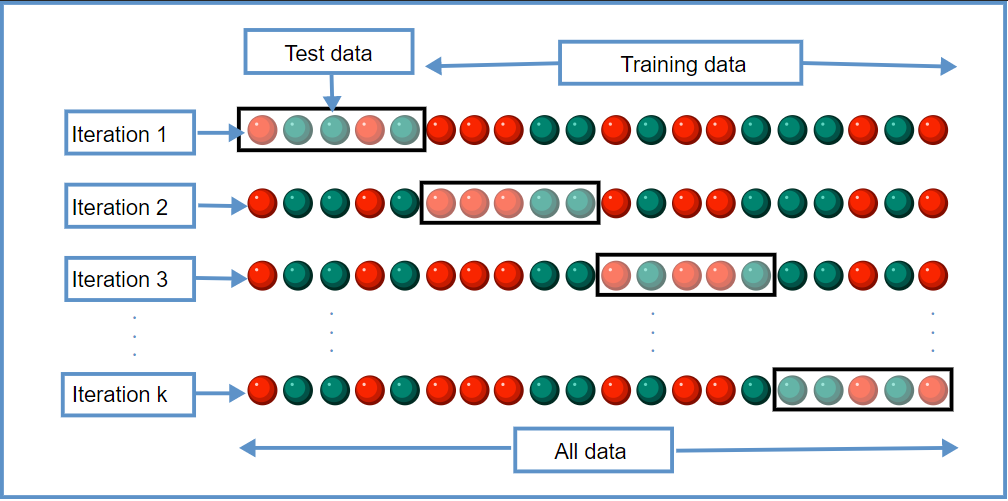
\includegraphics[width=650px]{images/CV} \textbackslash caption\{Cross validation from \href{https://en.wikipedia.org/wiki/Cross-validation_(statistics)}{wiki}; training data = used for building model; test data = used for prediction from the model that was built using training data; each iteration = fold\}\label{fig:cvpic}
\textbackslash end\{figure\}

\hypertarget{cross-validation-using-caret}{%
\subsubsection{Cross-validation using caret}\label{cross-validation-using-caret}}

We use \texttt{caret} package to do cross-validation.

\begin{rmdcomment}
\texttt{caret} is a general framework package for machine learning that
can also incorporate other ML approaches such as \texttt{xgboost}.
\end{rmdcomment}

\begin{Shaded}
\begin{Highlighting}[]
\FunctionTok{require}\NormalTok{(caret)}
\FunctionTok{set.seed}\NormalTok{(}\DecValTok{123}\NormalTok{)}
\NormalTok{X\_ObsData.matrix }\OtherTok{\textless{}{-}} \FunctionTok{xgb.DMatrix}\NormalTok{(ObsData.matrix)}
\NormalTok{Y\_ObsData }\OtherTok{\textless{}{-}}\NormalTok{ ObsData}\SpecialCharTok{$}\NormalTok{Y}
\end{Highlighting}
\end{Shaded}

Below we define \(K = 3\) for cross-validation. Ideally for a sample size close to \(n=5,000\), we would select \(K=10\), but for learning / demonstration / computational time-saving purposes, we just use \(K = 3\).

\begin{Shaded}
\begin{Highlighting}[]
\NormalTok{xgb\_trcontrol }\OtherTok{=} \FunctionTok{trainControl}\NormalTok{(}
  \AttributeTok{method =} \StringTok{"cv"}\NormalTok{,}
  \AttributeTok{number =} \DecValTok{3}\NormalTok{,  }
  \AttributeTok{allowParallel =} \ConstantTok{TRUE}\NormalTok{,}
  \AttributeTok{verboseIter =} \ConstantTok{FALSE}\NormalTok{,}
  \AttributeTok{returnData =} \ConstantTok{FALSE}
\NormalTok{)}
\end{Highlighting}
\end{Shaded}

\hypertarget{fine-tuning}{%
\subsubsection{Fine tuning}\label{fine-tuning}}

\begin{rmdcomment}
One of the advantages of \texttt{caret} framework is that, it also
allows checking the impact of various parameters (can do \textbf{fine
tuning}).
\end{rmdcomment}

For example,

\begin{itemize}
\tightlist
\item
  for interaction depth, we previously use \texttt{max.depth\ =\ 10}. That means \(covariate^{10}\) polynomial.
\item
  We could also check if other interaction depth choices (such as \(covariate^{2}\) or \(covariate^{4}\)) would be better in terms of honest predictions.
\end{itemize}

\begin{Shaded}
\begin{Highlighting}[]
\NormalTok{xgbGrid }\OtherTok{\textless{}{-}} \FunctionTok{expand.grid}\NormalTok{(}
  \AttributeTok{nrounds =} \DecValTok{100}\NormalTok{, }
  \AttributeTok{max\_depth =} \FunctionTok{seq}\NormalTok{(}\DecValTok{2}\NormalTok{,}\DecValTok{10}\NormalTok{,}\DecValTok{2}\NormalTok{),}
  \AttributeTok{eta =} \DecValTok{1}\NormalTok{,}
  \AttributeTok{gamma =} \DecValTok{0}\NormalTok{,}
  \AttributeTok{colsample\_bytree =} \FloatTok{0.1}\NormalTok{,}
  \AttributeTok{min\_child\_weight =} \DecValTok{2}\NormalTok{,}
  \AttributeTok{subsample =} \FloatTok{0.5} 
\NormalTok{)}
\end{Highlighting}
\end{Shaded}

\hypertarget{fit-model-with-cv}{%
\subsubsection{Fit model with CV}\label{fit-model-with-cv}}

once we set

\begin{itemize}
\tightlist
\item
  resampling or cross-validation settings
\item
  parameter grid
\end{itemize}

we can fit the model:

\begin{Shaded}
\begin{Highlighting}[]
\NormalTok{fit.xgb }\OtherTok{\textless{}{-}} \FunctionTok{train}\NormalTok{(}
\NormalTok{  X\_ObsData.matrix, Y\_ObsData,  }
  \AttributeTok{trControl =}\NormalTok{ xgb\_trcontrol,}
  \AttributeTok{method =} \StringTok{"xgbTree"}\NormalTok{,}
  \AttributeTok{tuneGrid =}\NormalTok{ xgbGrid,}
  \AttributeTok{verbose =} \ConstantTok{FALSE}
\NormalTok{)}
\NormalTok{fit.xgb}
\end{Highlighting}
\end{Shaded}

\begin{verbatim}
## eXtreme Gradient Boosting 
## 
## No pre-processing
## Resampling: Cross-Validated (3 fold) 
## Summary of sample sizes: 3822, 3824, 3824 
## Resampling results across tuning parameters:
## 
##   max_depth  RMSE      Rsquared     MAE     
##    2         28.87561  0.020524186  19.08176
##    4         38.88354  0.007198028  28.08175
##    6         49.62373  0.002200636  37.69929
##    8         54.86092  0.004255366  42.40188
##   10         57.13972  0.001224946  44.15276
## 
## Tuning parameter 'nrounds' was held constant at a value of 100
## Tuning
##  held constant at a value of 2
## Tuning parameter 'subsample' was held
##  constant at a value of 0.5
## RMSE was used to select the optimal model using the smallest value.
## The final values used for the model were nrounds = 100, max_depth = 2, eta =
##  1, gamma = 0, colsample_bytree = 0.1, min_child_weight = 2 and subsample = 0.5.
\end{verbatim}

Based on the loss function (say, RMSE) it automatically chose the best tuning parameter set:

\begin{Shaded}
\begin{Highlighting}[]
\NormalTok{fit.xgb}\SpecialCharTok{$}\NormalTok{bestTune}\SpecialCharTok{$}\NormalTok{max\_depth}
\end{Highlighting}
\end{Shaded}

\begin{verbatim}
## [1] 2
\end{verbatim}

\begin{Shaded}
\begin{Highlighting}[]
\NormalTok{predY }\OtherTok{\textless{}{-}} \FunctionTok{predict}\NormalTok{(fit.xgb, }\AttributeTok{newdata =}\NormalTok{ ObsData.matrix)}
\FunctionTok{plot}\NormalTok{(}\FunctionTok{density}\NormalTok{(Y), }
     \AttributeTok{col =} \StringTok{"red"}\NormalTok{, }
     \AttributeTok{main =} \StringTok{"Predicted and observed Y"}\NormalTok{,}
     \AttributeTok{xlim =} \FunctionTok{c}\NormalTok{(}\DecValTok{1}\NormalTok{,}\DecValTok{100}\NormalTok{))  }
\FunctionTok{legend}\NormalTok{(}\StringTok{"topright"}\NormalTok{, }
       \FunctionTok{c}\NormalTok{(}\StringTok{"Y"}\NormalTok{,}\StringTok{"Predicted Y"}\NormalTok{), }
       \AttributeTok{lty =} \FunctionTok{c}\NormalTok{(}\DecValTok{1}\NormalTok{,}\DecValTok{2}\NormalTok{), }
       \AttributeTok{col =} \FunctionTok{c}\NormalTok{(}\StringTok{"red"}\NormalTok{,}\StringTok{"blue"}\NormalTok{))}
\FunctionTok{lines}\NormalTok{(}\FunctionTok{density}\NormalTok{(predY), }\AttributeTok{col =} \StringTok{"blue"}\NormalTok{, }\AttributeTok{lty =} \DecValTok{2}\NormalTok{)}
\end{Highlighting}
\end{Shaded}

\includegraphics{TMLEw_files/figure-latex/unnamed-chunk-29-1.pdf}

\begin{Shaded}
\begin{Highlighting}[]
\NormalTok{caret}\SpecialCharTok{::}\FunctionTok{RMSE}\NormalTok{(predY,Y)}
\end{Highlighting}
\end{Shaded}

\begin{verbatim}
## [1] 24.35099
\end{verbatim}

\hypertarget{g-comp-step-2-extract-outcome-prediction-as-if-everyone-is-treated}{%
\subsection{G-comp step 2: Extract outcome prediction as if everyone is treated}\label{g-comp-step-2-extract-outcome-prediction-as-if-everyone-is-treated}}

\begin{Shaded}
\begin{Highlighting}[]
\NormalTok{ObsData.matrix.A1 }\OtherTok{\textless{}{-}}\NormalTok{ ObsData.matrix }
\NormalTok{ObsData.matrix.A1[,}\StringTok{"A"}\NormalTok{] }\OtherTok{\textless{}{-}} \DecValTok{1}
\NormalTok{ObsData}\SpecialCharTok{$}\NormalTok{Pred.Y1 }\OtherTok{\textless{}{-}} \FunctionTok{predict}\NormalTok{(fit.xgb, }\AttributeTok{newdata =}\NormalTok{ ObsData.matrix.A1)}
\FunctionTok{summary}\NormalTok{(ObsData}\SpecialCharTok{$}\NormalTok{Pred.Y1)}
\end{Highlighting}
\end{Shaded}

\begin{verbatim}
##    Min. 1st Qu.  Median    Mean 3rd Qu.    Max. 
##  -33.15   14.87   23.09   23.89   31.78  131.48
\end{verbatim}

\hypertarget{g-comp-step-3-extract-outcome-prediction-as-if-everyone-is-untreated}{%
\subsection{G-comp step 3: Extract outcome prediction as if everyone is untreated}\label{g-comp-step-3-extract-outcome-prediction-as-if-everyone-is-untreated}}

\begin{Shaded}
\begin{Highlighting}[]
\NormalTok{ObsData.matrix.A0 }\OtherTok{\textless{}{-}}\NormalTok{ ObsData.matrix}
\NormalTok{ObsData.matrix.A0[,}\StringTok{"A"}\NormalTok{] }\OtherTok{\textless{}{-}} \DecValTok{0}
\NormalTok{ObsData}\SpecialCharTok{$}\NormalTok{Pred.Y0 }\OtherTok{\textless{}{-}} \FunctionTok{predict}\NormalTok{(fit.xgb, }\AttributeTok{newdata =}\NormalTok{ ObsData.matrix.A0)}
\FunctionTok{summary}\NormalTok{(ObsData}\SpecialCharTok{$}\NormalTok{Pred.Y0)}
\end{Highlighting}
\end{Shaded}

\begin{verbatim}
##    Min. 1st Qu.  Median    Mean 3rd Qu.    Max. 
##  -37.31   10.72   18.96   19.78   27.69  127.31
\end{verbatim}

\hypertarget{g-comp-step-4-treatment-effect-estimate}{%
\subsection{G-comp step 4: Treatment effect estimate}\label{g-comp-step-4-treatment-effect-estimate}}

\begin{Shaded}
\begin{Highlighting}[]
\NormalTok{ObsData}\SpecialCharTok{$}\NormalTok{Pred.TE }\OtherTok{\textless{}{-}}\NormalTok{ ObsData}\SpecialCharTok{$}\NormalTok{Pred.Y1 }\SpecialCharTok{{-}}\NormalTok{ ObsData}\SpecialCharTok{$}\NormalTok{Pred.Y0  }
\end{Highlighting}
\end{Shaded}

Mean value of predicted treatment effect

\begin{Shaded}
\begin{Highlighting}[]
\NormalTok{TE1 }\OtherTok{\textless{}{-}} \FunctionTok{mean}\NormalTok{(ObsData}\SpecialCharTok{$}\NormalTok{Pred.TE)}
\NormalTok{TE1}
\end{Highlighting}
\end{Shaded}

\begin{verbatim}
## [1] 4.110383
\end{verbatim}

\begin{Shaded}
\begin{Highlighting}[]
\FunctionTok{summary}\NormalTok{(ObsData}\SpecialCharTok{$}\NormalTok{Pred.TE)}
\end{Highlighting}
\end{Shaded}

\begin{verbatim}
##    Min. 1st Qu.  Median    Mean 3rd Qu.    Max. 
##  -5.494   4.165   4.165   4.110   4.165   9.339
\end{verbatim}

Notice that the mean is slightly different than the parametric G-computation method.

\hypertarget{g-comp-using-regularized-methods}{%
\section{G-comp using regularized methods}\label{g-comp-using-regularized-methods}}

\hypertarget{a-regularized-model}{%
\subsection{A regularized model}\label{a-regularized-model}}

\begin{rmdcomment}
LASSO is a regularized method. One of the uses of these methods is
``variable selection'' or addressing concerns of multicollinearity.
\end{rmdcomment}

Let us use this method to fit our data.

\begin{itemize}
\tightlist
\item
  We are again using cross-validation here, and we chose \(K=3\).
\end{itemize}

\begin{Shaded}
\begin{Highlighting}[]
\FunctionTok{require}\NormalTok{(glmnet)}
\NormalTok{Y }\OtherTok{\textless{}{-}}\NormalTok{ObsData}\SpecialCharTok{$}\NormalTok{Y}
\NormalTok{ObsData.matrix }\OtherTok{\textless{}{-}} \FunctionTok{model.matrix}\NormalTok{(out.formula, }\AttributeTok{data =}\NormalTok{ ObsData)}
\NormalTok{fit4 }\OtherTok{\textless{}{-}}  \FunctionTok{cv.glmnet}\NormalTok{(}\AttributeTok{x =}\NormalTok{ ObsData.matrix, }
                \AttributeTok{y =}\NormalTok{ Y,}
                \AttributeTok{alpha =} \DecValTok{1}\NormalTok{,}
                \AttributeTok{nfolds =} \DecValTok{3}\NormalTok{,}
                \AttributeTok{relax=}\ConstantTok{TRUE}\NormalTok{)}
\end{Highlighting}
\end{Shaded}

\hypertarget{g-comp-step-2-extract-outcome-prediction-as-if-everyone-is-treated-1}{%
\subsection{G-comp step 2: Extract outcome prediction as if everyone is treated}\label{g-comp-step-2-extract-outcome-prediction-as-if-everyone-is-treated-1}}

\begin{Shaded}
\begin{Highlighting}[]
\NormalTok{ObsData.matrix.A1 }\OtherTok{\textless{}{-}}\NormalTok{ ObsData.matrix }
\NormalTok{ObsData.matrix.A1[,}\StringTok{"A"}\NormalTok{] }\OtherTok{\textless{}{-}} \DecValTok{1}
\NormalTok{ObsData}\SpecialCharTok{$}\NormalTok{Pred.Y1 }\OtherTok{\textless{}{-}} \FunctionTok{predict}\NormalTok{(fit4, }\AttributeTok{newx =}\NormalTok{ ObsData.matrix.A1,}
                           \AttributeTok{s =} \StringTok{"lambda.min"}\NormalTok{)}
\FunctionTok{summary}\NormalTok{(ObsData}\SpecialCharTok{$}\NormalTok{Pred.Y1)}
\end{Highlighting}
\end{Shaded}

\begin{verbatim}
##    lambda.min    
##  Min.   :-30.41  
##  1st Qu.: 19.53  
##  Median : 23.95  
##  Mean   : 23.24  
##  3rd Qu.: 27.26  
##  Max.   : 38.14
\end{verbatim}

\hypertarget{g-comp-step-3-extract-outcome-prediction-as-if-everyone-is-untreated-1}{%
\subsection{G-comp step 3: Extract outcome prediction as if everyone is untreated}\label{g-comp-step-3-extract-outcome-prediction-as-if-everyone-is-untreated-1}}

\begin{Shaded}
\begin{Highlighting}[]
\NormalTok{ObsData.matrix.A0 }\OtherTok{\textless{}{-}}\NormalTok{ ObsData.matrix}
\NormalTok{ObsData.matrix.A0[,}\StringTok{"A"}\NormalTok{] }\OtherTok{\textless{}{-}} \DecValTok{0}
\NormalTok{ObsData}\SpecialCharTok{$}\NormalTok{Pred.Y0 }\OtherTok{\textless{}{-}} \FunctionTok{predict}\NormalTok{(fit4, }\AttributeTok{newx =}\NormalTok{ ObsData.matrix.A0,}
                           \AttributeTok{s =} \StringTok{"lambda.min"}\NormalTok{)}
\FunctionTok{summary}\NormalTok{(ObsData}\SpecialCharTok{$}\NormalTok{Pred.Y0)}
\end{Highlighting}
\end{Shaded}

\begin{verbatim}
##    lambda.min    
##  Min.   :-33.13  
##  1st Qu.: 16.81  
##  Median : 21.23  
##  Mean   : 20.52  
##  3rd Qu.: 24.54  
##  Max.   : 35.42
\end{verbatim}

\hypertarget{g-comp-step-3-treatment-effect-estimate}{%
\subsection{G-comp step 3: Treatment effect estimate}\label{g-comp-step-3-treatment-effect-estimate}}

\begin{Shaded}
\begin{Highlighting}[]
\NormalTok{ObsData}\SpecialCharTok{$}\NormalTok{Pred.TE }\OtherTok{\textless{}{-}}\NormalTok{ ObsData}\SpecialCharTok{$}\NormalTok{Pred.Y1 }\SpecialCharTok{{-}}\NormalTok{ ObsData}\SpecialCharTok{$}\NormalTok{Pred.Y0  }
\end{Highlighting}
\end{Shaded}

Mean value of predicted treatment effect

\begin{Shaded}
\begin{Highlighting}[]
\NormalTok{TE2 }\OtherTok{\textless{}{-}} \FunctionTok{mean}\NormalTok{(ObsData}\SpecialCharTok{$}\NormalTok{Pred.TE)}
\NormalTok{TE2}
\end{Highlighting}
\end{Shaded}

\begin{verbatim}
## [1] 2.719739
\end{verbatim}

\begin{Shaded}
\begin{Highlighting}[]
\FunctionTok{summary}\NormalTok{(ObsData}\SpecialCharTok{$}\NormalTok{Pred.TE)}
\end{Highlighting}
\end{Shaded}

\begin{verbatim}
##    lambda.min  
##  Min.   :2.72  
##  1st Qu.:2.72  
##  Median :2.72  
##  Mean   :2.72  
##  3rd Qu.:2.72  
##  Max.   :2.72
\end{verbatim}

Notice that the mean is very similar to the parametric G-computation method.

\hypertarget{g-comp-using-superlearner}{%
\section{G-comp using SuperLearner}\label{g-comp-using-superlearner}}

\begin{rmdcomment}
SuperLearner is an ensemble ML technique, that uses
\textbf{cross-validation} to find a weighted combination of estimates
provided by different \textbf{candidate learners} (that help predict).
\end{rmdcomment}

\begin{itemize}
\tightlist
\item
  There exists many candidate learners. Here we are using a combination of

  \begin{itemize}
  \tightlist
  \item
    linear regression
  \item
    Regularized regression (lasso)
  \item
    gradient boosting (tree based)
  \end{itemize}
\end{itemize}

\hypertarget{steps-1}{%
\subsection{Steps}\label{steps-1}}

\begin{longtable}[]{@{}ll@{}}
\toprule
\endhead
Step 1 & Identify candidate learners\tabularnewline
Step 2 & Choose Cross-validation K\tabularnewline
Step 3 & Select loss function for meta learner\tabularnewline
Step 4 & Find SL prediction: (1) Discrete SL (2) Ensamble SL\tabularnewline
\bottomrule
\end{longtable}

\hypertarget{identify-candidate-learners}{%
\subsubsection{Identify candidate learners}\label{identify-candidate-learners}}

\begin{itemize}
\tightlist
\item
  Choose variety of candidate learners

  \begin{itemize}
  \tightlist
  \item
    parametric (linear or logistic regression)
  \item
    regularized (LASSO, ridge, elasticnet)
  \item
    stepwise
  \item
    non-parametric
  \item
    transformation (SVM, NN)
  \item
    tree based (bagging, boosting)
  \item
    smoothing or spline (gam)
  \end{itemize}
\item
  tune the candidate learners for better performance

  \begin{itemize}
  \tightlist
  \item
    tree depth
  \item
    tune regularization parameters
  \item
    variable selection
  \end{itemize}
\end{itemize}

\begin{Shaded}
\begin{Highlighting}[]
\NormalTok{SL.library.chosen}\OtherTok{=}\FunctionTok{c}\NormalTok{(}\StringTok{"SL.glm"}\NormalTok{, }\StringTok{"SL.glmnet"}\NormalTok{, }\StringTok{"SL.xgboost"}\NormalTok{)}
\end{Highlighting}
\end{Shaded}

\textbf{SuperLearner} is an ensemble learning method. Let us use this one to fit the data first.

\hypertarget{choose-cross-validation-k}{%
\subsubsection{Choose Cross-validation K}\label{choose-cross-validation-k}}

To combat against optimism, we use cross-validation. SuperLearner first \textbf{splits} the data according to chosen \(K\) fold for the cross-validation.

\begin{Shaded}
\begin{Highlighting}[]
\NormalTok{cvControl.chosen }\OtherTok{=} \FunctionTok{list}\NormalTok{(}\AttributeTok{V =} \DecValTok{3}\NormalTok{)}
\end{Highlighting}
\end{Shaded}

\hypertarget{select-loss-function-for-meta-learner-and-estimate-risk}{%
\subsubsection{Select loss function for meta learner and estimate risk}\label{select-loss-function-for-meta-learner-and-estimate-risk}}

\begin{rmdcomment}
The goal is to minimize the estimated risk (i.e., minimize the
difference of \(Y\) and \(\hat{Y}\)) that comes out of a model.
\end{rmdcomment}

We can chose a (non-negative) least squares loss function for the meta learner (explained below):

\begin{Shaded}
\begin{Highlighting}[]
\NormalTok{loss.chosen }\OtherTok{=} \StringTok{"method.NNLS"}
\end{Highlighting}
\end{Shaded}

\hypertarget{find-sl-prediction}{%
\subsubsection{Find SL prediction}\label{find-sl-prediction}}

We first fit the super learner:

\begin{Shaded}
\begin{Highlighting}[]
\FunctionTok{require}\NormalTok{(SuperLearner)}
\NormalTok{ObsData.noY }\OtherTok{\textless{}{-}}\NormalTok{ dplyr}\SpecialCharTok{::}\FunctionTok{select}\NormalTok{(ObsData, }\SpecialCharTok{!}\NormalTok{Y)}
\NormalTok{fit.sl }\OtherTok{\textless{}{-}} \FunctionTok{SuperLearner}\NormalTok{(}\AttributeTok{Y=}\NormalTok{ObsData}\SpecialCharTok{$}\NormalTok{Y, }
                       \AttributeTok{X=}\NormalTok{ObsData.noY, }
                       \AttributeTok{cvControl =}\NormalTok{ cvControl.chosen,}
                       \AttributeTok{SL.library=}\NormalTok{SL.library.chosen,}
                       \AttributeTok{method=}\NormalTok{loss.chosen,}
                       \AttributeTok{family=}\StringTok{"gaussian"}\NormalTok{)}
\end{Highlighting}
\end{Shaded}

We can also obtain the predictions from each candidate learners.

\begin{Shaded}
\begin{Highlighting}[]
\NormalTok{all.pred }\OtherTok{\textless{}{-}} \FunctionTok{predict}\NormalTok{(fit.sl, }\AttributeTok{type =} \StringTok{"response"}\NormalTok{)}
\NormalTok{Yhat }\OtherTok{\textless{}{-}}\NormalTok{ all.pred}\SpecialCharTok{$}\NormalTok{library.predict}
\FunctionTok{head}\NormalTok{(Yhat)}
\end{Highlighting}
\end{Shaded}

\begin{verbatim}
##   SL.glm_All SL.glmnet_All SL.xgboost_All
## 1   14.61647      14.57121      14.890952
## 2   28.66305      28.96897      42.775368
## 3   24.57800      24.98479      49.592552
## 4   18.70422      19.20871      25.078993
## 5   13.64956      12.18804       8.819989
## 6   22.56895      21.60971      11.892698
\end{verbatim}

We can obtain the \(K\)-fold cross-validated risk estimates for each candidate learners.

\begin{Shaded}
\begin{Highlighting}[]
\NormalTok{fit.sl}\SpecialCharTok{$}\NormalTok{cvRisk}
\end{Highlighting}
\end{Shaded}

\begin{verbatim}
##     SL.glm_All  SL.glmnet_All SL.xgboost_All 
##       634.4393       622.8681       737.5505
\end{verbatim}

Once we have the performance measures and predictions from candidate learners, we could go one of \textbf{two routes} here

\hypertarget{discrete-sl}{%
\paragraph{Discrete SL}\label{discrete-sl}}

\begin{rmdcomment}
Get measure of performance from all folds are averaged, and choose the
\textbf{best} one. The prediction from the chosen learners are then
used.
\end{rmdcomment}

\texttt{glmnet} has the lowest cross-validated risk

\begin{Shaded}
\begin{Highlighting}[]
\NormalTok{lowest.risk.learner }\OtherTok{\textless{}{-}} \FunctionTok{names}\NormalTok{(}\FunctionTok{which}\NormalTok{(}
\NormalTok{  fit.sl}\SpecialCharTok{$}\NormalTok{cvRisk }\SpecialCharTok{==} \FunctionTok{min}\NormalTok{(fit.sl}\SpecialCharTok{$}\NormalTok{cvRisk)))}
\NormalTok{lowest.risk.learner}
\end{Highlighting}
\end{Shaded}

\begin{verbatim}
## [1] "SL.glmnet_All"
\end{verbatim}

\begin{Shaded}
\begin{Highlighting}[]
\FunctionTok{as.matrix}\NormalTok{(}\FunctionTok{head}\NormalTok{(Yhat[,lowest.risk.learner]), }
          \AttributeTok{ncol=}\DecValTok{1}\NormalTok{)}
\end{Highlighting}
\end{Shaded}

\begin{verbatim}
##       [,1]
## 1 14.57121
## 2 28.96897
## 3 24.98479
## 4 19.20871
## 5 12.18804
## 6 21.60971
\end{verbatim}

\hypertarget{ensamble-sl}{%
\paragraph{Ensamble SL}\label{ensamble-sl}}

Here are the first 6 rows from the candidate learner predictions:

\begin{Shaded}
\begin{Highlighting}[]
\FunctionTok{head}\NormalTok{(Yhat)}
\end{Highlighting}
\end{Shaded}

\begin{verbatim}
##   SL.glm_All SL.glmnet_All SL.xgboost_All
## 1   14.61647      14.57121      14.890952
## 2   28.66305      28.96897      42.775368
## 3   24.57800      24.98479      49.592552
## 4   18.70422      19.20871      25.078993
## 5   13.64956      12.18804       8.819989
## 6   22.56895      21.60971      11.892698
\end{verbatim}

\begin{rmdcomment}
fit a \textbf{meta learner} (optimal weighted combination; below is a
simplified description)
\end{rmdcomment}

\begin{itemize}
\item
  using

  \begin{itemize}
  \tightlist
  \item
    linear regression (without intercept, but could produce -ve coefs) or
  \item
    preferably non-negative least squares for
  \end{itemize}

  \(Y_{obs}\) \(\sim\) \(\hat{Y}_{SL.glm}\) + \(\hat{Y}_{SL.glmnet}\) + \(\hat{Y}_{SL.xgboost}\).
\item
  Obtain the regression coefs \(\mathbf{\beta}\) = (\(\beta_{SL.glm}\), \(\beta_{SL.glmnet}\), \(\beta_{SL.xgboost}\)) for each \(\hat{Y}\),
\item
  scale them to 1

  \begin{itemize}
  \tightlist
  \item
    \(\mathbf{\beta_{scaled}}\) = \(\mathbf{\beta}\) / \(\sum_{i=1}^3{\mathbf{\beta}}\);
  \item
    so that the sum of scaled coefs = 1
  \end{itemize}
\item
  Scaled coefficients \(\mathbf{\beta_{scaled}}\) represents the \textbf{value / importance of the corresponding candidate learner}.
\end{itemize}

Scaled coefs

\begin{Shaded}
\begin{Highlighting}[]
\NormalTok{fit.sl}\SpecialCharTok{$}\NormalTok{coef}
\end{Highlighting}
\end{Shaded}

\begin{verbatim}
##     SL.glm_All  SL.glmnet_All SL.xgboost_All 
##     0.00000000     0.93740912     0.06259088
\end{verbatim}

\begin{Shaded}
\begin{Highlighting}[]
\FunctionTok{sum}\NormalTok{(fit.sl}\SpecialCharTok{$}\NormalTok{coef)}
\end{Highlighting}
\end{Shaded}

\begin{verbatim}
## [1] 1
\end{verbatim}

Hence, in creating superlearner prediction column,

\begin{enumerate}
\def\labelenumi{\alph{enumi}.}
\tightlist
\item
  Linear regression has no contribution
\item
  lasso has majority contribution
\item
  gradient boosting of tree has some minimal contribution
\end{enumerate}

\begin{itemize}
\tightlist
\item
  A new prediction column is produced based on the fitted values from this meta regression.
\end{itemize}

You can simply multiply these coefs to the predictions from candidate learners, and them sum them to get ensable SL. Here are the first 6 values:

\begin{Shaded}
\begin{Highlighting}[]
\NormalTok{SL.ens }\OtherTok{\textless{}{-}} \FunctionTok{t}\NormalTok{(}\FunctionTok{t}\NormalTok{(Yhat)}\SpecialCharTok{*}\NormalTok{fit.sl}\SpecialCharTok{$}\NormalTok{coef)}
\FunctionTok{head}\NormalTok{(SL.ens)}
\end{Highlighting}
\end{Shaded}

\begin{verbatim}
##   SL.glm_All SL.glmnet_All SL.xgboost_All
## 1          0      13.65919      0.9320378
## 2          0      27.15577      2.6773480
## 3          0      23.42097      3.1040416
## 4          0      18.00642      1.5697163
## 5          0      11.42518      0.5520509
## 6          0      20.25714      0.7443745
\end{verbatim}

\begin{Shaded}
\begin{Highlighting}[]
\FunctionTok{as.matrix}\NormalTok{(}\FunctionTok{head}\NormalTok{(}\FunctionTok{rowSums}\NormalTok{(SL.ens)), }\AttributeTok{ncol =} \DecValTok{1}\NormalTok{)}
\end{Highlighting}
\end{Shaded}

\begin{verbatim}
##       [,1]
## 1 14.59123
## 2 29.83312
## 3 26.52501
## 4 19.57614
## 5 11.97723
## 6 21.00152
\end{verbatim}

Alternatively, you can get them directly from the package: here are the first 6 values

\begin{Shaded}
\begin{Highlighting}[]
\FunctionTok{head}\NormalTok{(all.pred}\SpecialCharTok{$}\NormalTok{pred)}
\end{Highlighting}
\end{Shaded}

\begin{verbatim}
##       [,1]
## 1 14.59123
## 2 29.83312
## 3 26.52501
## 4 19.57614
## 5 11.97723
## 6 21.00152
\end{verbatim}

The last column is coming from Ensamble SL.

\hypertarget{g-comp-step-2-extract-outcome-prediction-as-if-everyone-is-treated-2}{%
\subsection{G-comp step 2: Extract outcome prediction as if everyone is treated}\label{g-comp-step-2-extract-outcome-prediction-as-if-everyone-is-treated-2}}

We are going to use \textbf{Ensamble SL} predictions in the following calculations. If you wanted to use discrete SL predictions instead, that would be fine too.

\begin{Shaded}
\begin{Highlighting}[]
\NormalTok{ObsData.noY}\SpecialCharTok{$}\NormalTok{A }\OtherTok{\textless{}{-}} \DecValTok{1}
\NormalTok{ObsData}\SpecialCharTok{$}\NormalTok{Pred.Y1 }\OtherTok{\textless{}{-}} \FunctionTok{predict}\NormalTok{(fit.sl, }\AttributeTok{newdata =}\NormalTok{ ObsData.noY,}
                           \AttributeTok{type =} \StringTok{"response"}\NormalTok{)}\SpecialCharTok{$}\NormalTok{pred}
\end{Highlighting}
\end{Shaded}

\begin{verbatim}
## Warning in predict.lm(object, newdata, se.fit, scale = 1, type = if (type == :
## prediction from a rank-deficient fit may be misleading
\end{verbatim}

\begin{Shaded}
\begin{Highlighting}[]
\FunctionTok{summary}\NormalTok{(ObsData}\SpecialCharTok{$}\NormalTok{Pred.Y1)}
\end{Highlighting}
\end{Shaded}

\begin{verbatim}
##        V1        
##  Min.   :-31.15  
##  1st Qu.: 18.70  
##  Median : 23.40  
##  Mean   : 22.75  
##  3rd Qu.: 27.09  
##  Max.   : 58.48
\end{verbatim}

\hypertarget{g-comp-step-3-extract-outcome-prediction-as-if-everyone-is-untreated-2}{%
\subsection{G-comp step 3: Extract outcome prediction as if everyone is untreated}\label{g-comp-step-3-extract-outcome-prediction-as-if-everyone-is-untreated-2}}

\begin{Shaded}
\begin{Highlighting}[]
\NormalTok{ObsData.noY}\SpecialCharTok{$}\NormalTok{A }\OtherTok{\textless{}{-}} \DecValTok{0}
\NormalTok{ObsData}\SpecialCharTok{$}\NormalTok{Pred.Y0 }\OtherTok{\textless{}{-}} \FunctionTok{predict}\NormalTok{(fit.sl, }\AttributeTok{newdata =}\NormalTok{ ObsData.noY,}
                           \AttributeTok{type =} \StringTok{"response"}\NormalTok{)}\SpecialCharTok{$}\NormalTok{pred}
\end{Highlighting}
\end{Shaded}

\begin{verbatim}
## Warning in predict.lm(object, newdata, se.fit, scale = 1, type = if (type == :
## prediction from a rank-deficient fit may be misleading
\end{verbatim}

\begin{Shaded}
\begin{Highlighting}[]
\FunctionTok{summary}\NormalTok{(ObsData}\SpecialCharTok{$}\NormalTok{Pred.Y0)}
\end{Highlighting}
\end{Shaded}

\begin{verbatim}
##        V1        
##  Min.   :-33.10  
##  1st Qu.: 16.76  
##  Median : 21.50  
##  Mean   : 20.83  
##  3rd Qu.: 25.18  
##  Max.   : 55.86
\end{verbatim}

\hypertarget{g-comp-step-3-treatment-effect-estimate-1}{%
\subsection{G-comp step 3: Treatment effect estimate}\label{g-comp-step-3-treatment-effect-estimate-1}}

\begin{Shaded}
\begin{Highlighting}[]
\NormalTok{ObsData}\SpecialCharTok{$}\NormalTok{Pred.TE }\OtherTok{\textless{}{-}}\NormalTok{ ObsData}\SpecialCharTok{$}\NormalTok{Pred.Y1 }\SpecialCharTok{{-}}\NormalTok{ ObsData}\SpecialCharTok{$}\NormalTok{Pred.Y0  }
\end{Highlighting}
\end{Shaded}

Mean value of predicted treatment effect

\begin{Shaded}
\begin{Highlighting}[]
\NormalTok{TE3 }\OtherTok{\textless{}{-}} \FunctionTok{mean}\NormalTok{(ObsData}\SpecialCharTok{$}\NormalTok{Pred.TE)}
\NormalTok{TE3}
\end{Highlighting}
\end{Shaded}

\begin{verbatim}
## [1] 1.914702
\end{verbatim}

\begin{Shaded}
\begin{Highlighting}[]
\FunctionTok{summary}\NormalTok{(ObsData}\SpecialCharTok{$}\NormalTok{Pred.TE)}
\end{Highlighting}
\end{Shaded}

\begin{verbatim}
##        V1       
##  Min.   :1.099  
##  1st Qu.:1.849  
##  Median :1.907  
##  Mean   :1.915  
##  3rd Qu.:1.976  
##  Max.   :2.991
\end{verbatim}

\hypertarget{additional-details-for-sl}{%
\subsection{Additional details for SL}\label{additional-details-for-sl}}

\hypertarget{choice-of-k}{%
\subsubsection{Choice of K}\label{choice-of-k}}

\begin{itemize}
\tightlist
\item
  simplest cross-validation splits the data into \(K=2\) parts, but can go higher.

  \begin{itemize}
  \tightlist
  \item
    select \(K\) judiciously

    \begin{itemize}
    \tightlist
    \item
      large sample size means small \(K\) may be adequate

      \begin{itemize}
      \tightlist
      \item
        for \(n \lt 10,000\) consider \(K=3\)
      \item
        for \(n \lt 500\) consider \(K=20\)
      \end{itemize}
    \item
      smaller sample size means larger \(K\) may be necessary

      \begin{itemize}
      \tightlist
      \item
        for \(n \lt 30\) consider leave 1 out
      \end{itemize}
    \end{itemize}
  \end{itemize}
\end{itemize}

\hypertarget{alternative-to-cv}{%
\subsubsection{Alternative to CV}\label{alternative-to-cv}}

\begin{itemize}
\tightlist
\item
  other similar algorithms such as \textbf{cross-fitting} had been shown to have better performances
\end{itemize}

\hypertarget{rare-outcome}{%
\subsubsection{Rare outcome}\label{rare-outcome}}

\begin{itemize}
\tightlist
\item
  for rare outcomes, consider using \textbf{stratification} to attempt to maintain training and test sample ratios the same
\end{itemize}

\hypertarget{dependant-sample}{%
\subsubsection{Dependant sample}\label{dependant-sample}}

\begin{itemize}
\tightlist
\item
  if data is clustered and not independent and identically distributed, use ID for the \textbf{cluster}
\end{itemize}

\hypertarget{choice-of-meta-learner-method}{%
\subsubsection{Choice of meta learner method}\label{choice-of-meta-learner-method}}

It is easy to show that, depending on the choice of meta-learners, the coefficients of the meta learners can be slightly different.

\begin{Shaded}
\begin{Highlighting}[]
\NormalTok{fit.sl2 }\OtherTok{\textless{}{-}} \FunctionTok{recombineSL}\NormalTok{(fit.sl, }\AttributeTok{Y =}\NormalTok{ Y, }
                       \AttributeTok{method =} \StringTok{"method.NNLS2"}\NormalTok{)}
\NormalTok{fit.sl2}\SpecialCharTok{$}\NormalTok{coef}
\end{Highlighting}
\end{Shaded}

\begin{verbatim}
##     SL.glm_All  SL.glmnet_All SL.xgboost_All 
##     0.00000000     0.93740912     0.06259088
\end{verbatim}

\begin{Shaded}
\begin{Highlighting}[]
\NormalTok{fit.sl2 }\OtherTok{\textless{}{-}} \FunctionTok{recombineSL}\NormalTok{(fit.sl, }\AttributeTok{Y =}\NormalTok{ Y, }
                       \AttributeTok{method =} \StringTok{"method.CC\_LS"}\NormalTok{)}
\NormalTok{fit.sl2}\SpecialCharTok{$}\NormalTok{coef}
\end{Highlighting}
\end{Shaded}

\begin{verbatim}
##     SL.glm_All  SL.glmnet_All SL.xgboost_All 
##     0.00000000     0.93662601     0.06337399
\end{verbatim}

\begin{Shaded}
\begin{Highlighting}[]
\NormalTok{fit.sl4 }\OtherTok{\textless{}{-}} \FunctionTok{recombineSL}\NormalTok{(fit.sl, }\AttributeTok{Y =}\NormalTok{ Y, }
                       \AttributeTok{method =} \StringTok{"method.CC\_nloglik"}\NormalTok{)}
\NormalTok{fit.sl4}\SpecialCharTok{$}\NormalTok{coef}
\end{Highlighting}
\end{Shaded}

\begin{verbatim}
##     SL.glm_All  SL.glmnet_All SL.xgboost_All 
##              0              1              0
\end{verbatim}

\begin{itemize}
\tightlist
\item
  \texttt{method.CC\_LS} is \href{https://si.biostat.washington.edu/sites/default/files/modules/lab1_0.pdf}{suggested} as a good method for continuous outcome
\item
  \texttt{method.CC\_nloglik} is \href{https://si.biostat.washington.edu/sites/default/files/modules/lab1_0.pdf}{suggested} as a good method for binary outcome
\end{itemize}

\begin{Shaded}
\begin{Highlighting}[]
\FunctionTok{saveRDS}\NormalTok{(TE1, }\AttributeTok{file =} \StringTok{"data/gcompxg.RDS"}\NormalTok{)}
\FunctionTok{saveRDS}\NormalTok{(TE2, }\AttributeTok{file =} \StringTok{"data/gcompls.RDS"}\NormalTok{)}
\FunctionTok{saveRDS}\NormalTok{(TE3, }\AttributeTok{file =} \StringTok{"data/gcompsl.RDS"}\NormalTok{)}
\end{Highlighting}
\end{Shaded}

\hypertarget{iptw}{%
\chapter{IPTW}\label{iptw}}

In this chapter, we will cover PS and IPTW (or IPW).

\begin{rmdcomment}
We are now primarily interested about \textbf{exposure modelling} (e.g.,
fixing imbalance first, before doing outcome analysis).
\end{rmdcomment}

\begin{Shaded}
\begin{Highlighting}[]
\CommentTok{\# Read the data saved at the last chapter}
\NormalTok{ObsData }\OtherTok{\textless{}{-}} \FunctionTok{readRDS}\NormalTok{(}\AttributeTok{file =} \StringTok{"data/rhcAnalytic.RDS"}\NormalTok{)}
\NormalTok{baselinevars }\OtherTok{\textless{}{-}} \FunctionTok{names}\NormalTok{(dplyr}\SpecialCharTok{::}\FunctionTok{select}\NormalTok{(ObsData, }\SpecialCharTok{!}\FunctionTok{c}\NormalTok{(A,Y)))}
\end{Highlighting}
\end{Shaded}

\hypertarget{iptw-steps}{%
\section{IPTW steps}\label{iptw-steps}}

\textbf{Modelling Steps}:

According to \citet{austin2011tutorial}, we need to follow 4 steps:

\begin{longtable}[]{@{}ll@{}}
\toprule
\endhead
Step 1 & exposure modelling: \(PS = Prob(A=1|L)\)\tabularnewline
Step 2 & Convert \(PS\) to \(IPW\) = \(\frac{A}{PS} + \frac{1-A}{1-PS}\)\tabularnewline
Step 3 & Assess balance in weighted sample (\(PS\) and \(L\))\tabularnewline
Step 4 & outcome modelling: \(E(Y|A=1)\) to obtain treatment effect estimate\tabularnewline
\bottomrule
\end{longtable}

\hypertarget{step-1-exposure-modelling}{%
\section{Step 1: exposure modelling}\label{step-1-exposure-modelling}}

\begin{rmdcomment}
Exposure modelling: \(PS = Prob(A=1|L)\)
\end{rmdcomment}

\begin{Shaded}
\begin{Highlighting}[]
\NormalTok{ps.formula }\OtherTok{\textless{}{-}} \FunctionTok{as.formula}\NormalTok{(}\FunctionTok{paste}\NormalTok{(}\StringTok{"A \textasciitilde{}"}\NormalTok{,}
                               \FunctionTok{paste}\NormalTok{(baselinevars,}
                                     \AttributeTok{collapse =} \StringTok{"+"}\NormalTok{)))}
\NormalTok{ps.formula}
\end{Highlighting}
\end{Shaded}

\begin{verbatim}
## A ~ Disease.category + Cancer + Cardiovascular + Congestive.HF + 
##     Dementia + Psychiatric + Pulmonary + Renal + Hepatic + GI.Bleed + 
##     Tumor + Immunosupperssion + Transfer.hx + MI + age + sex + 
##     edu + DASIndex + APACHE.score + Glasgow.Coma.Score + blood.pressure + 
##     WBC + Heart.rate + Respiratory.rate + Temperature + PaO2vs.FIO2 + 
##     Albumin + Hematocrit + Bilirubin + Creatinine + Sodium + 
##     Potassium + PaCo2 + PH + Weight + DNR.status + Medical.insurance + 
##     Respiratory.Diag + Cardiovascular.Diag + Neurological.Diag + 
##     Gastrointestinal.Diag + Renal.Diag + Metabolic.Diag + Hematologic.Diag + 
##     Sepsis.Diag + Trauma.Diag + Orthopedic.Diag + race + income
\end{verbatim}

\begin{itemize}
\tightlist
\item
  Other than main effect terms, what other model specifications are possible?

  \begin{itemize}
  \tightlist
  \item
    Common terms to add (indeed based on biological plausibility; requiring subject area knowledge)
  \item
    Interactions
  \item
    polynomials or splines
  \item
    transformations
  \end{itemize}
\end{itemize}

Fit logistic regression to estimate propensity scores

\begin{Shaded}
\begin{Highlighting}[]
\NormalTok{PS.fit }\OtherTok{\textless{}{-}} \FunctionTok{glm}\NormalTok{(ps.formula,}\AttributeTok{family=}\StringTok{"binomial"}\NormalTok{, }\AttributeTok{data=}\NormalTok{ObsData)}
\FunctionTok{require}\NormalTok{(Publish)}
\FunctionTok{publish}\NormalTok{(PS.fit,  }\AttributeTok{format =} \StringTok{"[u;l]"}\NormalTok{)}
\end{Highlighting}
\end{Shaded}

\begin{verbatim}
##               Variable               Units OddsRatio        CI.95     p-value 
##       Disease.category                 ARF       Ref                          
##                                        CHF      1.79  [1.32;2.43]   0.0002047 
##                                      Other      0.54  [0.43;0.68]     < 1e-04 
##                                       MOSF      1.58  [1.34;1.87]     < 1e-04 
##                 Cancer                None       Ref                          
##                            Localized (Yes)      0.46  [0.22;0.96]   0.0389310 
##                                 Metastatic      0.37  [0.17;0.81]   0.0131229 
##         Cardiovascular                   0       Ref                          
##                                          1      1.04  [0.86;1.25]   0.7036980 
##          Congestive.HF                   0       Ref                          
##                                          1      1.10  [0.90;1.35]   0.3461245 
##               Dementia                   0       Ref                          
##                                          1      0.67  [0.53;0.85]   0.0011382 
##            Psychiatric                   0       Ref                          
##                                          1      0.65  [0.50;0.85]   0.0018616 
##              Pulmonary                   0       Ref                          
##                                          1      0.97  [0.81;1.18]   0.7814947 
##                  Renal                   0       Ref                          
##                                          1      0.70  [0.49;1.00]   0.0523978 
##                Hepatic                   0       Ref                          
##                                          1      0.79  [0.57;1.11]   0.1817681 
##               GI.Bleed                   0       Ref                          
##                                          1      0.76  [0.49;1.17]   0.2148665 
##                  Tumor                   0       Ref                          
##                                          1      1.48  [0.71;3.12]   0.2987694 
##      Immunosupperssion                   0       Ref                          
##                                          1      1.00  [0.86;1.15]   0.9778387 
##            Transfer.hx                   0       Ref                          
##                                          1      1.46  [1.20;1.77]   0.0001356 
##                     MI                   0       Ref                          
##                                          1      1.12  [0.80;1.59]   0.5031463 
##                    age           [-Inf,50)       Ref                          
##                                    [50,60)      1.04  [0.85;1.27]   0.7327200 
##                                    [60,70)      1.22  [1.00;1.49]   0.0559205 
##                                    [70,80)      1.15  [0.91;1.45]   0.2414163 
##                                  [80, Inf)      0.66  [0.49;0.89]   0.0054612 
##                    sex                Male       Ref                          
##                                     Female      0.98  [0.86;1.12]   0.7661356 
##                    edu                          1.03  [1.01;1.05]   0.0101741 
##               DASIndex                          1.00  [0.98;1.01]   0.6635060 
##           APACHE.score                          1.01  [1.01;1.02]     < 1e-04 
##     Glasgow.Coma.Score                          1.00  [1.00;1.00]   0.2853053 
##         blood.pressure                          0.99  [0.99;0.99]     < 1e-04 
##                    WBC                          1.00  [0.99;1.00]   0.7368619 
##             Heart.rate                          1.00  [1.00;1.01]     < 1e-04 
##       Respiratory.rate                          0.98  [0.97;0.98]     < 1e-04 
##            Temperature                          0.97  [0.93;1.01]   0.1255016 
##            PaO2vs.FIO2                          0.99  [0.99;1.00]     < 1e-04 
##                Albumin                          0.93  [0.85;1.02]   0.1032557 
##             Hematocrit                          0.99  [0.98;1.00]   0.0103236 
##              Bilirubin                          1.01  [1.00;1.02]   0.1719966 
##             Creatinine                          1.04  [1.00;1.09]   0.0576310 
##                 Sodium                          0.99  [0.98;1.00]   0.0049192 
##              Potassium                          0.85  [0.79;0.91]     < 1e-04 
##                  PaCo2                          0.98  [0.97;0.98]     < 1e-04 
##                     PH                          0.22  [0.11;0.47]     < 1e-04 
##                 Weight                          1.01  [1.00;1.01]     < 1e-04 
##             DNR.status                  No       Ref                          
##                                        Yes      0.58  [0.46;0.73]     < 1e-04 
##      Medical.insurance            Medicaid       Ref                          
##                                   Medicare      1.34  [1.03;1.74]   0.0315228 
##                        Medicare & Medicaid      1.49  [1.07;2.07]   0.0184712 
##                               No insurance      1.66  [1.20;2.30]   0.0023684 
##                                    Private      1.55  [1.21;1.97]   0.0004402 
##                         Private & Medicare      1.46  [1.11;1.92]   0.0071028 
##       Respiratory.Diag                  No       Ref                          
##                                        Yes      0.76  [0.65;0.90]   0.0010144 
##    Cardiovascular.Diag                  No       Ref                          
##                                        Yes      1.80  [1.52;2.13]     < 1e-04 
##      Neurological.Diag                  No       Ref                          
##                                        Yes      0.62  [0.47;0.80]   0.0002731 
##  Gastrointestinal.Diag                  No       Ref                          
##                                        Yes      1.41  [1.15;1.73]   0.0010690 
##             Renal.Diag                  No       Ref                          
##                                        Yes      1.35  [1.01;1.80]   0.0461405 
##         Metabolic.Diag                  No       Ref                          
##                                        Yes      0.85  [0.63;1.15]   0.2953120 
##       Hematologic.Diag                  No       Ref                          
##                                        Yes      0.59  [0.45;0.78]   0.0002225 
##            Sepsis.Diag                  No       Ref                          
##                                        Yes      1.31  [1.10;1.57]   0.0029968 
##            Trauma.Diag                  No       Ref                          
##                                        Yes      3.45  [1.80;6.64]   0.0002014 
##        Orthopedic.Diag                  No       Ref                          
##                                        Yes      3.74 [0.53;26.25]   0.1843027 
##                   race               white       Ref                          
##                                      black      1.05  [0.87;1.26]   0.6250189 
##                                      other      1.09  [0.84;1.41]   0.5272282 
##                 income            $11-$25k       Ref                          
##                                   $25-$50k      1.08  [0.87;1.34]   0.4644703 
##                                     > $50k      1.02  [0.78;1.34]   0.8810245 
##                                 Under $11k      1.06  [0.90;1.26]   0.4797051
\end{verbatim}

\begin{rmdcomment}
Coef of PS model fit is not of concern.
\end{rmdcomment}

\begin{itemize}
\tightlist
\item
  Model can be rich: to the extent that prediction is better
\item
  But look for multi-collinearity issues

  \begin{itemize}
  \tightlist
  \item
    SE too high?
  \end{itemize}
\end{itemize}

Obtain the propesnity score (PS) values from the fit

\begin{Shaded}
\begin{Highlighting}[]
\NormalTok{ObsData}\SpecialCharTok{$}\NormalTok{PS }\OtherTok{\textless{}{-}} \FunctionTok{predict}\NormalTok{(PS.fit, }\AttributeTok{type=}\StringTok{"response"}\NormalTok{)}
\end{Highlighting}
\end{Shaded}

\begin{rmdcomment}
These propensity score predictions (\texttt{PS}) are often represented
as \(g(A_i=1|L_i)\).
\end{rmdcomment}

Check summaries:

\begin{itemize}
\tightlist
\item
  enough overlap?
\item
  PS values very close to 0 or 1?
\end{itemize}

\begin{Shaded}
\begin{Highlighting}[]
\FunctionTok{summary}\NormalTok{(ObsData}\SpecialCharTok{$}\NormalTok{PS)}
\end{Highlighting}
\end{Shaded}

\begin{verbatim}
##     Min.  1st Qu.   Median     Mean  3rd Qu.     Max. 
## 0.002478 0.161446 0.358300 0.380819 0.574319 0.968425
\end{verbatim}

\begin{Shaded}
\begin{Highlighting}[]
\FunctionTok{tapply}\NormalTok{(ObsData}\SpecialCharTok{$}\NormalTok{PS, ObsData}\SpecialCharTok{$}\NormalTok{A, summary)}
\end{Highlighting}
\end{Shaded}

\begin{verbatim}
## $`0`
##     Min.  1st Qu.   Median     Mean  3rd Qu.     Max. 
## 0.002478 0.106718 0.241301 0.283816 0.427138 0.951927 
## 
## $`1`
##    Min. 1st Qu.  Median    Mean 3rd Qu.    Max. 
## 0.01575 0.37205 0.55243 0.53854 0.70999 0.96842
\end{verbatim}

\begin{Shaded}
\begin{Highlighting}[]
\FunctionTok{plot}\NormalTok{(}\FunctionTok{density}\NormalTok{(ObsData}\SpecialCharTok{$}\NormalTok{PS[ObsData}\SpecialCharTok{$}\NormalTok{A}\SpecialCharTok{==}\DecValTok{0}\NormalTok{]), }
     \AttributeTok{col =} \StringTok{"red"}\NormalTok{, }\AttributeTok{main =} \StringTok{""}\NormalTok{)}
\FunctionTok{lines}\NormalTok{(}\FunctionTok{density}\NormalTok{(ObsData}\SpecialCharTok{$}\NormalTok{PS[ObsData}\SpecialCharTok{$}\NormalTok{A}\SpecialCharTok{==}\DecValTok{1}\NormalTok{]), }
      \AttributeTok{col =} \StringTok{"blue"}\NormalTok{, }\AttributeTok{lty =} \DecValTok{2}\NormalTok{)}
\FunctionTok{legend}\NormalTok{(}\StringTok{"topright"}\NormalTok{, }\FunctionTok{c}\NormalTok{(}\StringTok{"No RHC"}\NormalTok{,}\StringTok{"RHC"}\NormalTok{), }
       \AttributeTok{col =} \FunctionTok{c}\NormalTok{(}\StringTok{"red"}\NormalTok{, }\StringTok{"blue"}\NormalTok{), }\AttributeTok{lty=}\DecValTok{1}\SpecialCharTok{:}\DecValTok{2}\NormalTok{)}
\end{Highlighting}
\end{Shaded}

\includegraphics{TMLEw_files/figure-latex/psx2b-1.pdf}

\hypertarget{step-2-convert-ps-to-ipw}{%
\section{Step 2: Convert PS to IPW}\label{step-2-convert-ps-to-ipw}}

\begin{rmdcomment}
Convert \(PS\) to \(IPW\) = \(\frac{A}{PS} + \frac{1-A}{1-PS}\)
\end{rmdcomment}

\begin{itemize}
\tightlist
\item
  Convert PS to IPW using the formula. We are using the formula for average treatment effect (ATE).
\end{itemize}

\begin{rmdcomment}
It is possible to use alternative formulas, but we are using ATE formula
for our illustration.
\end{rmdcomment}

\begin{Shaded}
\begin{Highlighting}[]
\NormalTok{ObsData}\SpecialCharTok{$}\NormalTok{IPW }\OtherTok{\textless{}{-}}\NormalTok{ ObsData}\SpecialCharTok{$}\NormalTok{A}\SpecialCharTok{/}\NormalTok{ObsData}\SpecialCharTok{$}\NormalTok{PS }\SpecialCharTok{+}\NormalTok{ (}\DecValTok{1}\SpecialCharTok{{-}}\NormalTok{ObsData}\SpecialCharTok{$}\NormalTok{A)}\SpecialCharTok{/}\NormalTok{(}\DecValTok{1}\SpecialCharTok{{-}}\NormalTok{ObsData}\SpecialCharTok{$}\NormalTok{PS)}
\FunctionTok{summary}\NormalTok{(ObsData}\SpecialCharTok{$}\NormalTok{IPW)}
\end{Highlighting}
\end{Shaded}

\begin{verbatim}
##    Min. 1st Qu.  Median    Mean 3rd Qu.    Max. 
##   1.002   1.183   1.472   1.986   2.064  63.509
\end{verbatim}

Also possible to use pre-packaged software packages to do the same:

\begin{Shaded}
\begin{Highlighting}[]
\FunctionTok{require}\NormalTok{(WeightIt)}
\NormalTok{W.out }\OtherTok{\textless{}{-}} \FunctionTok{weightit}\NormalTok{(ps.formula, }
                    \AttributeTok{data =}\NormalTok{ ObsData, }
                    \AttributeTok{estimand =} \StringTok{"ATE"}\NormalTok{,}
                    \AttributeTok{method =} \StringTok{"ps"}\NormalTok{)}
\FunctionTok{summary}\NormalTok{(W.out}\SpecialCharTok{$}\NormalTok{weights)}
\end{Highlighting}
\end{Shaded}

\begin{verbatim}
##    Min. 1st Qu.  Median    Mean 3rd Qu.    Max. 
##   1.002   1.183   1.472   1.986   2.064  63.509
\end{verbatim}

\hypertarget{step-3-balance-checking}{%
\section{Step 3: Balance checking}\label{step-3-balance-checking}}

\begin{rmdcomment}
Assess balance in weighted sample (\(PS\) and \(L\))
\end{rmdcomment}

We can check balance numerically.

\begin{itemize}
\tightlist
\item
  We set SMD = 0.1 as threshold for balance.
\item
  \(SMD \gt 0.1\) means we do not have balance
\end{itemize}

\begin{Shaded}
\begin{Highlighting}[]
\FunctionTok{require}\NormalTok{(cobalt)}
\FunctionTok{bal.tab}\NormalTok{(W.out, }\AttributeTok{un =} \ConstantTok{TRUE}\NormalTok{, }
        \AttributeTok{thresholds =} \FunctionTok{c}\NormalTok{(}\AttributeTok{m =}\NormalTok{ .}\DecValTok{1}\NormalTok{))}
\end{Highlighting}
\end{Shaded}

\begin{verbatim}
## Call
##  weightit(formula = ps.formula, data = ObsData, method = "ps", 
##     estimand = "ATE")
## 
## Balance Measures
##                                           Type Diff.Un Diff.Adj    M.Threshold
## prop.score                            Distance  1.1926   0.0224 Balanced, <0.1
## Disease.category_ARF                    Binary -0.0290   0.0025 Balanced, <0.1
## Disease.category_CHF                    Binary  0.0261   0.0008 Balanced, <0.1
## Disease.category_Other                  Binary -0.1737  -0.0080 Balanced, <0.1
## Disease.category_MOSF                   Binary  0.1766   0.0047 Balanced, <0.1
## Cancer_None                             Binary  0.0439   0.0017 Balanced, <0.1
## Cancer_Localized (Yes)                  Binary -0.0267   0.0017 Balanced, <0.1
## Cancer_Metastatic                       Binary -0.0172  -0.0034 Balanced, <0.1
## Cardiovascular                          Binary  0.0445   0.0051 Balanced, <0.1
## Congestive.HF                           Binary  0.0268   0.0013 Balanced, <0.1
## Dementia                                Binary -0.0472  -0.0138 Balanced, <0.1
## Psychiatric                             Binary -0.0348  -0.0050 Balanced, <0.1
## Pulmonary                               Binary -0.0737  -0.0058 Balanced, <0.1
## Renal                                   Binary  0.0066   0.0027 Balanced, <0.1
## Hepatic                                 Binary -0.0124  -0.0012 Balanced, <0.1
## GI.Bleed                                Binary -0.0122  -0.0026 Balanced, <0.1
## Tumor                                   Binary -0.0423  -0.0016 Balanced, <0.1
## Immunosupperssion                       Binary  0.0358  -0.0027 Balanced, <0.1
## Transfer.hx                             Binary  0.0554   0.0047 Balanced, <0.1
## MI                                      Binary  0.0139   0.0005 Balanced, <0.1
## age_[-Inf,50)                           Binary -0.0017  -0.0098 Balanced, <0.1
## age_[50,60)                             Binary  0.0161   0.0149 Balanced, <0.1
## age_[60,70)                             Binary  0.0355  -0.0108 Balanced, <0.1
## age_[70,80)                             Binary  0.0144   0.0047 Balanced, <0.1
## age_[80, Inf)                           Binary -0.0643   0.0010 Balanced, <0.1
## sex_Female                              Binary -0.0462  -0.0143 Balanced, <0.1
## edu                                    Contin.  0.0914  -0.0000 Balanced, <0.1
## DASIndex                               Contin.  0.0626   0.0435 Balanced, <0.1
## APACHE.score                           Contin.  0.5014   0.0109 Balanced, <0.1
## Glasgow.Coma.Score                     Contin. -0.1098   0.0034 Balanced, <0.1
## blood.pressure                         Contin. -0.4551   0.0057 Balanced, <0.1
## WBC                                    Contin.  0.0836   0.0470 Balanced, <0.1
## Heart.rate                             Contin.  0.1469   0.0210 Balanced, <0.1
## Respiratory.rate                       Contin. -0.1655   0.0037 Balanced, <0.1
## Temperature                            Contin. -0.0214   0.0090 Balanced, <0.1
## PaO2vs.FIO2                            Contin. -0.4332  -0.0016 Balanced, <0.1
## Albumin                                Contin. -0.2299  -0.0279 Balanced, <0.1
## Hematocrit                             Contin. -0.2693  -0.0247 Balanced, <0.1
## Bilirubin                              Contin.  0.1446  -0.0069 Balanced, <0.1
## Creatinine                             Contin.  0.2696   0.0148 Balanced, <0.1
## Sodium                                 Contin. -0.0922  -0.0059 Balanced, <0.1
## Potassium                              Contin. -0.0271  -0.0264 Balanced, <0.1
## PaCo2                                  Contin. -0.2486  -0.0201 Balanced, <0.1
## PH                                     Contin. -0.1198   0.0095 Balanced, <0.1
## Weight                                 Contin.  0.2557   0.0209 Balanced, <0.1
## DNR.status_Yes                          Binary -0.0696  -0.0112 Balanced, <0.1
## Medical.insurance_Medicaid              Binary -0.0395   0.0058 Balanced, <0.1
## Medical.insurance_Medicare              Binary -0.0327  -0.0119 Balanced, <0.1
## Medical.insurance_Medicare & Medicaid   Binary -0.0144  -0.0001 Balanced, <0.1
## Medical.insurance_No insurance          Binary  0.0099  -0.0002 Balanced, <0.1
## Medical.insurance_Private               Binary  0.0624   0.0013 Balanced, <0.1
## Medical.insurance_Private & Medicare    Binary  0.0143   0.0052 Balanced, <0.1
## Respiratory.Diag_Yes                    Binary -0.1277  -0.0056 Balanced, <0.1
## Cardiovascular.Diag_Yes                 Binary  0.1395   0.0034 Balanced, <0.1
## Neurological.Diag_Yes                   Binary -0.1079  -0.0038 Balanced, <0.1
## Gastrointestinal.Diag_Yes               Binary  0.0453  -0.0028 Balanced, <0.1
## Renal.Diag_Yes                          Binary  0.0264   0.0021 Balanced, <0.1
## Metabolic.Diag_Yes                      Binary -0.0059   0.0002 Balanced, <0.1
## Hematologic.Diag_Yes                    Binary -0.0146  -0.0000 Balanced, <0.1
## Sepsis.Diag_Yes                         Binary  0.0912   0.0035 Balanced, <0.1
## Trauma.Diag_Yes                         Binary  0.0105   0.0011 Balanced, <0.1
## Orthopedic.Diag_Yes                     Binary  0.0010   0.0002 Balanced, <0.1
## race_white                              Binary  0.0063  -0.0030 Balanced, <0.1
## race_black                              Binary -0.0114   0.0067 Balanced, <0.1
## race_other                              Binary  0.0050  -0.0036 Balanced, <0.1
## income_$11-$25k                         Binary  0.0062  -0.0096 Balanced, <0.1
## income_$25-$50k                         Binary  0.0391   0.0032 Balanced, <0.1
## income_> $50k                           Binary  0.0165  -0.0001 Balanced, <0.1
## income_Under $11k                       Binary -0.0618   0.0065 Balanced, <0.1
## 
## Balance tally for mean differences
##                    count
## Balanced, <0.1        69
## Not Balanced, >0.1     0
## 
## Variable with the greatest mean difference
##  Variable Diff.Adj    M.Threshold
##       WBC    0.047 Balanced, <0.1
## 
## Effective sample sizes
##            Control Treated
## Unadjusted 3551.   2184.  
## Adjusted   2532.46 1039.44
\end{verbatim}

\begin{itemize}
\tightlist
\item
  We can also check this in a plot
\end{itemize}

\begin{Shaded}
\begin{Highlighting}[]
\FunctionTok{require}\NormalTok{(cobalt)}
\FunctionTok{love.plot}\NormalTok{(W.out, }\AttributeTok{binary =} \StringTok{"std"}\NormalTok{,}
          \AttributeTok{thresholds =} \FunctionTok{c}\NormalTok{(}\AttributeTok{m =}\NormalTok{ .}\DecValTok{1}\NormalTok{),}
          \AttributeTok{abs =} \ConstantTok{TRUE}\NormalTok{, }
          \AttributeTok{var.order =} \StringTok{"unadjusted"}\NormalTok{, }
          \AttributeTok{line =} \ConstantTok{TRUE}\NormalTok{)}
\end{Highlighting}
\end{Shaded}

\includegraphics{TMLEw_files/figure-latex/balp2-1.pdf}

\begin{rmdcomment}
All covariates are balanced! Reverse engineered an RCT!?!
\end{rmdcomment}

\hypertarget{step-4-outcome-modelling}{%
\section{Step 4: outcome modelling}\label{step-4-outcome-modelling}}

\begin{rmdcomment}
Outcome modelling: \(E(Y|A=1)\) to obtain treatment effect estimate
\end{rmdcomment}

Estimate the effect of treatment on outcomes

\begin{Shaded}
\begin{Highlighting}[]
\NormalTok{out.formula }\OtherTok{\textless{}{-}} \FunctionTok{as.formula}\NormalTok{(Y }\SpecialCharTok{\textasciitilde{}}\NormalTok{ A)}
\NormalTok{out.fit }\OtherTok{\textless{}{-}} \FunctionTok{glm}\NormalTok{(out.formula,}
               \AttributeTok{data =}\NormalTok{ ObsData,}
               \AttributeTok{weights =}\NormalTok{ IPW)}
\FunctionTok{publish}\NormalTok{(out.fit)}
\end{Highlighting}
\end{Shaded}

\begin{verbatim}
##     Variable Units Coefficient         CI.95 p-value 
##  (Intercept)             20.68 [19.73;21.64] < 1e-04 
##            A              3.24   [1.88;4.60] < 1e-04
\end{verbatim}

\begin{Shaded}
\begin{Highlighting}[]
\FunctionTok{saveRDS}\NormalTok{(out.fit, }\AttributeTok{file =} \StringTok{"data/ipw.RDS"}\NormalTok{)}
\end{Highlighting}
\end{Shaded}

\hypertarget{iptw-using-ml}{%
\chapter{IPTW using ML}\label{iptw-using-ml}}

Similar to G-computation, we will try to use machine learning methods, particularly Superlearner in estimating IPW estimates

\begin{Shaded}
\begin{Highlighting}[]
\CommentTok{\# Read the data saved at the last chapter}
\NormalTok{ObsData }\OtherTok{\textless{}{-}} \FunctionTok{readRDS}\NormalTok{(}\AttributeTok{file =} \StringTok{"data/rhcAnalytic.RDS"}\NormalTok{)}
\NormalTok{baselinevars }\OtherTok{\textless{}{-}} \FunctionTok{names}\NormalTok{(dplyr}\SpecialCharTok{::}\FunctionTok{select}\NormalTok{(ObsData, }\SpecialCharTok{!}\FunctionTok{c}\NormalTok{(A,Y)))}
\NormalTok{ps.formula }\OtherTok{\textless{}{-}} \FunctionTok{as.formula}\NormalTok{(}\FunctionTok{paste}\NormalTok{(}\StringTok{"A \textasciitilde{}"}\NormalTok{,}
                               \FunctionTok{paste}\NormalTok{(baselinevars,}
                                     \AttributeTok{collapse =} \StringTok{"+"}\NormalTok{)))}
\end{Highlighting}
\end{Shaded}

\hypertarget{iptw-steps-from-sl}{%
\section{IPTW Steps from SL}\label{iptw-steps-from-sl}}

\textbf{Modelling Steps}:

We will still follow the same steps

\begin{longtable}[]{@{}ll@{}}
\toprule
\endhead
\begin{minipage}[t]{(\columnwidth - 1\tabcolsep) * \real{0.50}}\raggedright
Step 1\strut
\end{minipage} & \begin{minipage}[t]{(\columnwidth - 1\tabcolsep) * \real{0.50}}\raggedright
exposure modelling: \(PS = Prob(A=1|L)\)\strut
\end{minipage}\tabularnewline
\begin{minipage}[t]{(\columnwidth - 1\tabcolsep) * \real{0.50}}\raggedright
Step 2\strut
\end{minipage} & \begin{minipage}[t]{(\columnwidth - 1\tabcolsep) * \real{0.50}}\raggedright
Convert \(PS\) to \(IPW\) = \(\frac{A}{PS} + \frac{1-A}{1-PS}\)\strut
\end{minipage}\tabularnewline
\begin{minipage}[t]{(\columnwidth - 1\tabcolsep) * \real{0.50}}\raggedright
Step 3\strut
\end{minipage} & \begin{minipage}[t]{(\columnwidth - 1\tabcolsep) * \real{0.50}}\raggedright
Assess balance in weighted sample and overlap (\(PS\) and \(L\))\strut
\end{minipage}\tabularnewline
\begin{minipage}[t]{(\columnwidth - 1\tabcolsep) * \real{0.50}}\raggedright
Step 4\strut
\end{minipage} & \begin{minipage}[t]{(\columnwidth - 1\tabcolsep) * \real{0.50}}\raggedright
outcome modelling: \(Prob(Y=1|A=1)\) to obtain treatment effect estimate\strut
\end{minipage}\tabularnewline
\bottomrule
\end{longtable}

\hypertarget{step-1-exposure-modelling-1}{%
\section{Step 1: exposure modelling}\label{step-1-exposure-modelling-1}}

This is the exposure model that we decided on:

\begin{Shaded}
\begin{Highlighting}[]
\NormalTok{ps.formula}
\end{Highlighting}
\end{Shaded}

\begin{verbatim}
## A ~ Disease.category + Cancer + Cardiovascular + Congestive.HF + 
##     Dementia + Psychiatric + Pulmonary + Renal + Hepatic + GI.Bleed + 
##     Tumor + Immunosupperssion + Transfer.hx + MI + age + sex + 
##     edu + DASIndex + APACHE.score + Glasgow.Coma.Score + blood.pressure + 
##     WBC + Heart.rate + Respiratory.rate + Temperature + PaO2vs.FIO2 + 
##     Albumin + Hematocrit + Bilirubin + Creatinine + Sodium + 
##     Potassium + PaCo2 + PH + Weight + DNR.status + Medical.insurance + 
##     Respiratory.Diag + Cardiovascular.Diag + Neurological.Diag + 
##     Gastrointestinal.Diag + Renal.Diag + Metabolic.Diag + Hematologic.Diag + 
##     Sepsis.Diag + Trauma.Diag + Orthopedic.Diag + race + income
\end{verbatim}

\begin{rmdcomment}
Fit SuperLearner (SL) to estimate propensity scores.
\end{rmdcomment}

We again use the same candidate learners:

\begin{itemize}
\tightlist
\item
  linear model
\item
  LASSO
\item
  gradient boosting
\end{itemize}

\begin{Shaded}
\begin{Highlighting}[]
\FunctionTok{require}\NormalTok{(SuperLearner)}
\NormalTok{ObsData.noYA }\OtherTok{\textless{}{-}}\NormalTok{ dplyr}\SpecialCharTok{::}\FunctionTok{select}\NormalTok{(ObsData, }\SpecialCharTok{!}\FunctionTok{c}\NormalTok{(Y,A))}
\NormalTok{PS.fit.SL }\OtherTok{\textless{}{-}} \FunctionTok{SuperLearner}\NormalTok{(}\AttributeTok{Y=}\NormalTok{ObsData}\SpecialCharTok{$}\NormalTok{A, }
                       \AttributeTok{X=}\NormalTok{ObsData.noYA, }
                       \AttributeTok{cvControl =} \FunctionTok{list}\NormalTok{(}\AttributeTok{V =} \DecValTok{3}\NormalTok{),}
                       \AttributeTok{SL.library=}\FunctionTok{c}\NormalTok{(}\StringTok{"SL.glm"}\NormalTok{, }\StringTok{"SL.glmnet"}\NormalTok{, }\StringTok{"SL.xgboost"}\NormalTok{), }
                       \AttributeTok{method=}\StringTok{"method.NNLS"}\NormalTok{,}
                       \AttributeTok{family=}\StringTok{"binomial"}\NormalTok{)}
\end{Highlighting}
\end{Shaded}

Here, \texttt{method.AUC} is also possible to use instead of \texttt{method.NNLS} for binary response. We could use \texttt{cvControl\ =\ list(V\ =\ 3,\ stratifyCV\ =\ TRUE)} to make the splits be stratified by the binary response.

Obtain the propesnity score (PS) values from the fit

\begin{Shaded}
\begin{Highlighting}[]
\NormalTok{all.pred }\OtherTok{\textless{}{-}} \FunctionTok{predict}\NormalTok{(PS.fit.SL, }\AttributeTok{type =} \StringTok{"response"}\NormalTok{)}
\NormalTok{ObsData}\SpecialCharTok{$}\NormalTok{PS.SL }\OtherTok{\textless{}{-}}\NormalTok{ all.pred}\SpecialCharTok{$}\NormalTok{pred}
\end{Highlighting}
\end{Shaded}

Check summaries:

\begin{Shaded}
\begin{Highlighting}[]
\FunctionTok{summary}\NormalTok{(ObsData}\SpecialCharTok{$}\NormalTok{PS.SL)}
\end{Highlighting}
\end{Shaded}

\begin{verbatim}
##        V1          
##  Min.   :0.002524  
##  1st Qu.:0.144662  
##  Median :0.343638  
##  Mean   :0.380834  
##  3rd Qu.:0.596531  
##  Max.   :0.973761
\end{verbatim}

\begin{Shaded}
\begin{Highlighting}[]
\FunctionTok{tapply}\NormalTok{(ObsData}\SpecialCharTok{$}\NormalTok{PS.SL, ObsData}\SpecialCharTok{$}\NormalTok{A, summary)}
\end{Highlighting}
\end{Shaded}

\begin{verbatim}
## $`0`
##     Min.  1st Qu.   Median     Mean  3rd Qu.     Max. 
## 0.002524 0.086511 0.186111 0.218359 0.324914 0.786757 
## 
## $`1`
##    Min. 1st Qu.  Median    Mean 3rd Qu.    Max. 
## 0.08064 0.52214 0.66185 0.64500 0.77675 0.97376
\end{verbatim}

\begin{Shaded}
\begin{Highlighting}[]
\FunctionTok{plot}\NormalTok{(}\FunctionTok{density}\NormalTok{(ObsData}\SpecialCharTok{$}\NormalTok{PS.SL[ObsData}\SpecialCharTok{$}\NormalTok{A}\SpecialCharTok{==}\DecValTok{0}\NormalTok{]), }
     \AttributeTok{col =} \StringTok{"red"}\NormalTok{, }\AttributeTok{main =} \StringTok{""}\NormalTok{)}
\FunctionTok{lines}\NormalTok{(}\FunctionTok{density}\NormalTok{(ObsData}\SpecialCharTok{$}\NormalTok{PS.SL[ObsData}\SpecialCharTok{$}\NormalTok{A}\SpecialCharTok{==}\DecValTok{1}\NormalTok{]), }
      \AttributeTok{col =} \StringTok{"blue"}\NormalTok{, }\AttributeTok{lty =} \DecValTok{2}\NormalTok{)}
\FunctionTok{legend}\NormalTok{(}\StringTok{"topright"}\NormalTok{, }\FunctionTok{c}\NormalTok{(}\StringTok{"No RHC"}\NormalTok{,}\StringTok{"RHC"}\NormalTok{), }
       \AttributeTok{col =} \FunctionTok{c}\NormalTok{(}\StringTok{"red"}\NormalTok{, }\StringTok{"blue"}\NormalTok{), }\AttributeTok{lty=}\DecValTok{1}\SpecialCharTok{:}\DecValTok{2}\NormalTok{)}
\end{Highlighting}
\end{Shaded}

\includegraphics{TMLEw_files/figure-latex/ipw2psx2b-1.pdf}

\hypertarget{step-2-convert-ps-to-ipw-1}{%
\section{Step 2: Convert PS to IPW}\label{step-2-convert-ps-to-ipw-1}}

\begin{itemize}
\tightlist
\item
  Convert PS from SL to IPW using the formula (again, ATE formula).
\end{itemize}

\begin{Shaded}
\begin{Highlighting}[]
\NormalTok{ObsData}\SpecialCharTok{$}\NormalTok{IPW.SL }\OtherTok{\textless{}{-}}\NormalTok{ ObsData}\SpecialCharTok{$}\NormalTok{A}\SpecialCharTok{/}\NormalTok{ObsData}\SpecialCharTok{$}\NormalTok{PS.SL }\SpecialCharTok{+}\NormalTok{ (}\DecValTok{1}\SpecialCharTok{{-}}\NormalTok{ObsData}\SpecialCharTok{$}\NormalTok{A)}\SpecialCharTok{/}\NormalTok{(}\DecValTok{1}\SpecialCharTok{{-}}\NormalTok{ObsData}\SpecialCharTok{$}\NormalTok{PS.SL)}
\FunctionTok{summary}\NormalTok{(ObsData}\SpecialCharTok{$}\NormalTok{IPW.SL)}
\end{Highlighting}
\end{Shaded}

\begin{verbatim}
##        V1        
##  Min.   : 1.003  
##  1st Qu.: 1.141  
##  Median : 1.324  
##  Mean   : 1.485  
##  3rd Qu.: 1.640  
##  Max.   :12.401
\end{verbatim}

Output from pre-packged software packages to do the same (very similar estimates):

\begin{Shaded}
\begin{Highlighting}[]
\FunctionTok{require}\NormalTok{(WeightIt)}
\NormalTok{W.out }\OtherTok{\textless{}{-}} \FunctionTok{weightit}\NormalTok{(ps.formula, }
                    \AttributeTok{data =}\NormalTok{ ObsData, }
                    \AttributeTok{estimand =} \StringTok{"ATE"}\NormalTok{,}
                    \AttributeTok{method =} \StringTok{"super"}\NormalTok{,}
                    \AttributeTok{SL.library =} \FunctionTok{c}\NormalTok{(}\StringTok{"SL.glm"}\NormalTok{, }
                                   \StringTok{"SL.glmnet"}\NormalTok{, }
                                   \StringTok{"SL.xgboost"}\NormalTok{))}
\FunctionTok{summary}\NormalTok{(W.out}\SpecialCharTok{$}\NormalTok{weights)}
\end{Highlighting}
\end{Shaded}

\begin{verbatim}
##    Min. 1st Qu.  Median    Mean 3rd Qu.    Max. 
##   1.002   1.134   1.314   1.470   1.627  12.884
\end{verbatim}

\begin{Shaded}
\begin{Highlighting}[]
\FunctionTok{saveRDS}\NormalTok{(W.out, }\AttributeTok{file =} \StringTok{"data/ipwslps.RDS"}\NormalTok{)}
\end{Highlighting}
\end{Shaded}

Alternatively, you can use the previously estimated PS

\begin{Shaded}
\begin{Highlighting}[]
\NormalTok{W.out2 }\OtherTok{\textless{}{-}} \FunctionTok{weightit}\NormalTok{(ps.formula, }
                    \AttributeTok{data =}\NormalTok{ ObsData, }
                    \AttributeTok{estimand =} \StringTok{"ATE"}\NormalTok{,}
                    \AttributeTok{ps =}\NormalTok{ ObsData}\SpecialCharTok{$}\NormalTok{PS.SL)}
\FunctionTok{summary}\NormalTok{(W.out2}\SpecialCharTok{$}\NormalTok{weights)}
\end{Highlighting}
\end{Shaded}

\begin{verbatim}
##    Min. 1st Qu.  Median    Mean 3rd Qu.    Max. 
##   1.003   1.141   1.324   1.485   1.640  12.401
\end{verbatim}

\hypertarget{step-3-balance-checking-1}{%
\section{Step 3: Balance checking}\label{step-3-balance-checking-1}}

\begin{itemize}
\tightlist
\item
  We first check balance numerically for SMD = 0.1 as threshold for balance.
\end{itemize}

\begin{Shaded}
\begin{Highlighting}[]
\FunctionTok{bal.tab}\NormalTok{(W.out, }\AttributeTok{un =} \ConstantTok{TRUE}\NormalTok{, }
        \AttributeTok{thresholds =} \FunctionTok{c}\NormalTok{(}\AttributeTok{m =}\NormalTok{ .}\DecValTok{1}\NormalTok{))}
\end{Highlighting}
\end{Shaded}

\begin{verbatim}
## Call
##  weightit(formula = ps.formula, data = ObsData, method = "super", 
##     estimand = "ATE", SL.library = c("SL.glm", "SL.glmnet", "SL.xgboost"))
## 
## Balance Measures
##                                           Type Diff.Un Diff.Adj
## prop.score                            Distance  2.6936   2.0928
## Disease.category_ARF                    Binary -0.0290  -0.0083
## Disease.category_CHF                    Binary  0.0261   0.0146
## Disease.category_Other                  Binary -0.1737  -0.1006
## Disease.category_MOSF                   Binary  0.1766   0.0943
## Cancer_None                             Binary  0.0439   0.0241
## Cancer_Localized (Yes)                  Binary -0.0267  -0.0130
## Cancer_Metastatic                       Binary -0.0172  -0.0112
## Cardiovascular                          Binary  0.0445   0.0276
## Congestive.HF                           Binary  0.0268   0.0151
## Dementia                                Binary -0.0472  -0.0292
## Psychiatric                             Binary -0.0348  -0.0199
## Pulmonary                               Binary -0.0737  -0.0422
## Renal                                   Binary  0.0066   0.0051
## Hepatic                                 Binary -0.0124  -0.0077
## GI.Bleed                                Binary -0.0122  -0.0078
## Tumor                                   Binary -0.0423  -0.0230
## Immunosupperssion                       Binary  0.0358   0.0192
## Transfer.hx                             Binary  0.0554   0.0274
## MI                                      Binary  0.0139   0.0071
## age_[-Inf,50)                           Binary -0.0017  -0.0022
## age_[50,60)                             Binary  0.0161   0.0123
## age_[60,70)                             Binary  0.0355   0.0157
## age_[70,80)                             Binary  0.0144   0.0104
## age_[80, Inf)                           Binary -0.0643  -0.0361
## sex_Female                              Binary -0.0462  -0.0274
## edu                                    Contin.  0.0914   0.0490
## DASIndex                               Contin.  0.0626   0.0404
## APACHE.score                           Contin.  0.5014   0.2628
## Glasgow.Coma.Score                     Contin. -0.1098  -0.0623
## blood.pressure                         Contin. -0.4551  -0.2388
## WBC                                    Contin.  0.0836   0.0526
## Heart.rate                             Contin.  0.1469   0.0803
## Respiratory.rate                       Contin. -0.1655  -0.0812
## Temperature                            Contin. -0.0214  -0.0037
## PaO2vs.FIO2                            Contin. -0.4332  -0.2325
## Albumin                                Contin. -0.2299  -0.1277
## Hematocrit                             Contin. -0.2693  -0.1570
## Bilirubin                              Contin.  0.1446   0.0753
## Creatinine                             Contin.  0.2696   0.1408
## Sodium                                 Contin. -0.0922  -0.0490
## Potassium                              Contin. -0.0271  -0.0265
## PaCo2                                  Contin. -0.2486  -0.1469
## PH                                     Contin. -0.1198  -0.0513
## Weight                                 Contin.  0.2557   0.1399
## DNR.status_Yes                          Binary -0.0696  -0.0422
## Medical.insurance_Medicaid              Binary -0.0395  -0.0218
## Medical.insurance_Medicare              Binary -0.0327  -0.0176
## Medical.insurance_Medicare & Medicaid   Binary -0.0144  -0.0070
## Medical.insurance_No insurance          Binary  0.0099   0.0058
## Medical.insurance_Private               Binary  0.0624   0.0326
## Medical.insurance_Private & Medicare    Binary  0.0143   0.0081
## Respiratory.Diag_Yes                    Binary -0.1277  -0.0664
## Cardiovascular.Diag_Yes                 Binary  0.1395   0.0750
## Neurological.Diag_Yes                   Binary -0.1079  -0.0586
## Gastrointestinal.Diag_Yes               Binary  0.0453   0.0241
## Renal.Diag_Yes                          Binary  0.0264   0.0143
## Metabolic.Diag_Yes                      Binary -0.0059  -0.0022
## Hematologic.Diag_Yes                    Binary -0.0146  -0.0080
## Sepsis.Diag_Yes                         Binary  0.0912   0.0478
## Trauma.Diag_Yes                         Binary  0.0105   0.0062
## Orthopedic.Diag_Yes                     Binary  0.0010   0.0006
## race_white                              Binary  0.0063   0.0044
## race_black                              Binary -0.0114  -0.0044
## race_other                              Binary  0.0050  -0.0001
## income_$11-$25k                         Binary  0.0062   0.0014
## income_$25-$50k                         Binary  0.0391   0.0203
## income_> $50k                           Binary  0.0165   0.0080
## income_Under $11k                       Binary -0.0618  -0.0298
##                                              M.Threshold
## prop.score                                              
## Disease.category_ARF                      Balanced, <0.1
## Disease.category_CHF                      Balanced, <0.1
## Disease.category_Other                Not Balanced, >0.1
## Disease.category_MOSF                     Balanced, <0.1
## Cancer_None                               Balanced, <0.1
## Cancer_Localized (Yes)                    Balanced, <0.1
## Cancer_Metastatic                         Balanced, <0.1
## Cardiovascular                            Balanced, <0.1
## Congestive.HF                             Balanced, <0.1
## Dementia                                  Balanced, <0.1
## Psychiatric                               Balanced, <0.1
## Pulmonary                                 Balanced, <0.1
## Renal                                     Balanced, <0.1
## Hepatic                                   Balanced, <0.1
## GI.Bleed                                  Balanced, <0.1
## Tumor                                     Balanced, <0.1
## Immunosupperssion                         Balanced, <0.1
## Transfer.hx                               Balanced, <0.1
## MI                                        Balanced, <0.1
## age_[-Inf,50)                             Balanced, <0.1
## age_[50,60)                               Balanced, <0.1
## age_[60,70)                               Balanced, <0.1
## age_[70,80)                               Balanced, <0.1
## age_[80, Inf)                             Balanced, <0.1
## sex_Female                                Balanced, <0.1
## edu                                       Balanced, <0.1
## DASIndex                                  Balanced, <0.1
## APACHE.score                          Not Balanced, >0.1
## Glasgow.Coma.Score                        Balanced, <0.1
## blood.pressure                        Not Balanced, >0.1
## WBC                                       Balanced, <0.1
## Heart.rate                                Balanced, <0.1
## Respiratory.rate                          Balanced, <0.1
## Temperature                               Balanced, <0.1
## PaO2vs.FIO2                           Not Balanced, >0.1
## Albumin                               Not Balanced, >0.1
## Hematocrit                            Not Balanced, >0.1
## Bilirubin                                 Balanced, <0.1
## Creatinine                            Not Balanced, >0.1
## Sodium                                    Balanced, <0.1
## Potassium                                 Balanced, <0.1
## PaCo2                                 Not Balanced, >0.1
## PH                                        Balanced, <0.1
## Weight                                Not Balanced, >0.1
## DNR.status_Yes                            Balanced, <0.1
## Medical.insurance_Medicaid                Balanced, <0.1
## Medical.insurance_Medicare                Balanced, <0.1
## Medical.insurance_Medicare & Medicaid     Balanced, <0.1
## Medical.insurance_No insurance            Balanced, <0.1
## Medical.insurance_Private                 Balanced, <0.1
## Medical.insurance_Private & Medicare      Balanced, <0.1
## Respiratory.Diag_Yes                      Balanced, <0.1
## Cardiovascular.Diag_Yes                   Balanced, <0.1
## Neurological.Diag_Yes                     Balanced, <0.1
## Gastrointestinal.Diag_Yes                 Balanced, <0.1
## Renal.Diag_Yes                            Balanced, <0.1
## Metabolic.Diag_Yes                        Balanced, <0.1
## Hematologic.Diag_Yes                      Balanced, <0.1
## Sepsis.Diag_Yes                           Balanced, <0.1
## Trauma.Diag_Yes                           Balanced, <0.1
## Orthopedic.Diag_Yes                       Balanced, <0.1
## race_white                                Balanced, <0.1
## race_black                                Balanced, <0.1
## race_other                                Balanced, <0.1
## income_$11-$25k                           Balanced, <0.1
## income_$25-$50k                           Balanced, <0.1
## income_> $50k                             Balanced, <0.1
## income_Under $11k                         Balanced, <0.1
## 
## Balance tally for mean differences
##                    count
## Balanced, <0.1        59
## Not Balanced, >0.1     9
## 
## Variable with the greatest mean difference
##      Variable Diff.Adj        M.Threshold
##  APACHE.score   0.2628 Not Balanced, >0.1
## 
## Effective sample sizes
##            Control Treated
## Unadjusted 3551.   2184.  
## Adjusted   3305.68 1884.77
\end{verbatim}

\begin{itemize}
\tightlist
\item
  And also via plot
\end{itemize}

\begin{Shaded}
\begin{Highlighting}[]
\FunctionTok{require}\NormalTok{(cobalt)}
\FunctionTok{love.plot}\NormalTok{(W.out, }\AttributeTok{binary =} \StringTok{"std"}\NormalTok{,}
          \AttributeTok{thresholds =} \FunctionTok{c}\NormalTok{(}\AttributeTok{m =}\NormalTok{ .}\DecValTok{1}\NormalTok{),}
          \AttributeTok{abs =} \ConstantTok{TRUE}\NormalTok{, }
          \AttributeTok{var.order =} \StringTok{"unadjusted"}\NormalTok{, }
          \AttributeTok{line =} \ConstantTok{TRUE}\NormalTok{)}
\end{Highlighting}
\end{Shaded}

\includegraphics{TMLEw_files/figure-latex/ipw2balp2-1.pdf}

\begin{rmdcomment}
Some covariates have SMD \textgreater{} 0.1 (sign of imbalance). This
phenomenon is common when we use strong ML methods to obtain PS
{[}@alam2019should{]}.
\end{rmdcomment}

\hypertarget{step-4-outcome-modelling-1}{%
\section{Step 4: outcome modelling}\label{step-4-outcome-modelling-1}}

Estimate the effect of treatment on outcomes

\hypertarget{crude}{%
\subsection{Crude}\label{crude}}

\begin{Shaded}
\begin{Highlighting}[]
\NormalTok{out.formula }\OtherTok{\textless{}{-}} \FunctionTok{as.formula}\NormalTok{(Y }\SpecialCharTok{\textasciitilde{}}\NormalTok{ A)}
\NormalTok{out.fit }\OtherTok{\textless{}{-}} \FunctionTok{glm}\NormalTok{(out.formula,}
               \AttributeTok{data =}\NormalTok{ ObsData,}
               \AttributeTok{weights =}\NormalTok{ IPW.SL)}
\FunctionTok{publish}\NormalTok{(out.fit)}
\end{Highlighting}
\end{Shaded}

\begin{verbatim}
##     Variable Units Coefficient         CI.95 p-value 
##  (Intercept)             20.20 [19.30;21.11] < 1e-04 
##            A              4.28   [2.91;5.64] < 1e-04
\end{verbatim}

\hypertarget{adjusted}{%
\subsection{Adjusted}\label{adjusted}}

\begin{rmdcomment}
Adjusting for all covariates to deal with potential residual confounding
(as was indicated by imbalance). Alternatively, could adjust for
selected covariates believed to be the reasons for potential imbalance
{[}@nguyen2017double{]}.
\end{rmdcomment}

Estimate the effect of treatment on outcomes (after adjustment)

\begin{Shaded}
\begin{Highlighting}[]
\NormalTok{out.formula2 }\OtherTok{\textless{}{-}} \FunctionTok{as.formula}\NormalTok{(}\FunctionTok{paste}\NormalTok{(}\StringTok{"Y\textasciitilde{} A +"}\NormalTok{, }
                               \FunctionTok{paste}\NormalTok{(baselinevars, }
                                     \AttributeTok{collapse =} \StringTok{"+"}\NormalTok{)))}
\NormalTok{out.fit2 }\OtherTok{\textless{}{-}} \FunctionTok{glm}\NormalTok{(out.formula2,}
               \AttributeTok{data =}\NormalTok{ ObsData,}
               \AttributeTok{weights =}\NormalTok{ IPW.SL)}
\NormalTok{res2 }\OtherTok{\textless{}{-}} \FunctionTok{publish}\NormalTok{(out.fit2, }\AttributeTok{digits=}\DecValTok{1}\NormalTok{)}\SpecialCharTok{$}\NormalTok{regressionTable[}\DecValTok{2}\NormalTok{,]}
\end{Highlighting}
\end{Shaded}

\begin{Shaded}
\begin{Highlighting}[]
\NormalTok{res2}
\end{Highlighting}
\end{Shaded}

 
  \providecommand{\huxb}[2]{\arrayrulecolor[RGB]{#1}\global\arrayrulewidth=#2pt}
  \providecommand{\huxvb}[2]{\color[RGB]{#1}\vrule width #2pt}
  \providecommand{\huxtpad}[1]{\rule{0pt}{#1}}
  \providecommand{\huxbpad}[1]{\rule[-#1]{0pt}{#1}}

\begin{table}[ht]
\begin{centerbox}
\begin{threeparttable}
\captionsetup{justification=centering,singlelinecheck=off}
\caption{\label{tab:ipw2psx4adj2} }
 \setlength{\tabcolsep}{0pt}
\begin{tabular}{l l l l l}


\hhline{>{\huxb{0, 0, 0}{0.4}}->{\huxb{0, 0, 0}{0.4}}->{\huxb{0, 0, 0}{0.4}}->{\huxb{0, 0, 0}{0.4}}->{\huxb{0, 0, 0}{0.4}}-}
\arrayrulecolor{black}

\multicolumn{1}{!{\huxvb{0, 0, 0}{0.4}}l!{\huxvb{0, 0, 0}{0}}}{\huxtpad{6pt + 1em}\raggedright \hspace{6pt} \textbf{Variable} \hspace{6pt}\huxbpad{6pt}} &
\multicolumn{1}{l!{\huxvb{0, 0, 0}{0}}}{\huxtpad{6pt + 1em}\raggedright \hspace{6pt} \textbf{Units} \hspace{6pt}\huxbpad{6pt}} &
\multicolumn{1}{l!{\huxvb{0, 0, 0}{0}}}{\huxtpad{6pt + 1em}\raggedright \hspace{6pt} \textbf{Coefficient} \hspace{6pt}\huxbpad{6pt}} &
\multicolumn{1}{l!{\huxvb{0, 0, 0}{0}}}{\huxtpad{6pt + 1em}\raggedright \hspace{6pt} \textbf{CI.95} \hspace{6pt}\huxbpad{6pt}} &
\multicolumn{1}{l!{\huxvb{0, 0, 0}{0.4}}}{\huxtpad{6pt + 1em}\raggedright \hspace{6pt} \textbf{p-value} \hspace{6pt}\huxbpad{6pt}} \tabularnewline[-0.5pt]


\hhline{>{\huxb{0, 0, 0}{0.4}}->{\huxb{0, 0, 0}{0.4}}->{\huxb{0, 0, 0}{0.4}}->{\huxb{0, 0, 0}{0.4}}->{\huxb{0, 0, 0}{0.4}}-}
\arrayrulecolor{black}

\multicolumn{1}{!{\huxvb{0, 0, 0}{0.4}}l!{\huxvb{0, 0, 0}{0}}}{\cellcolor[RGB]{242, 242, 242}\huxtpad{6pt + 1em}\raggedright \hspace{6pt} A \hspace{6pt}\huxbpad{6pt}} &
\multicolumn{1}{l!{\huxvb{0, 0, 0}{0}}}{\cellcolor[RGB]{242, 242, 242}\huxtpad{6pt + 1em}\raggedright \hspace{6pt}  \hspace{6pt}\huxbpad{6pt}} &
\multicolumn{1}{l!{\huxvb{0, 0, 0}{0}}}{\cellcolor[RGB]{242, 242, 242}\huxtpad{6pt + 1em}\raggedright \hspace{6pt} 2.9 \hspace{6pt}\huxbpad{6pt}} &
\multicolumn{1}{l!{\huxvb{0, 0, 0}{0}}}{\cellcolor[RGB]{242, 242, 242}\huxtpad{6pt + 1em}\raggedright \hspace{6pt} [1.5;4.3] \hspace{6pt}\huxbpad{6pt}} &
\multicolumn{1}{l!{\huxvb{0, 0, 0}{0.4}}}{\cellcolor[RGB]{242, 242, 242}\huxtpad{6pt + 1em}\raggedright \hspace{6pt} $<$0.1 \hspace{6pt}\huxbpad{6pt}} \tabularnewline[-0.5pt]


\hhline{>{\huxb{0, 0, 0}{0.4}}->{\huxb{0, 0, 0}{0.4}}->{\huxb{0, 0, 0}{0.4}}->{\huxb{0, 0, 0}{0.4}}->{\huxb{0, 0, 0}{0.4}}-}
\arrayrulecolor{black}
\end{tabular}
\end{threeparttable}\par\end{centerbox}

\end{table}
 

\hypertarget{adjusted-from-package}{%
\subsection{Adjusted (from package)}\label{adjusted-from-package}}

Also check the output when we used the weights from the package

\begin{Shaded}
\begin{Highlighting}[]
\NormalTok{out.fit3 }\OtherTok{\textless{}{-}} \FunctionTok{glm}\NormalTok{(out.formula2,}
               \AttributeTok{data =}\NormalTok{ ObsData,}
               \AttributeTok{weights =}\NormalTok{ W.out}\SpecialCharTok{$}\NormalTok{weights)}
\NormalTok{res3 }\OtherTok{\textless{}{-}} \FunctionTok{publish}\NormalTok{(out.fit3, }\AttributeTok{digits=}\DecValTok{1}\NormalTok{)}\SpecialCharTok{$}\NormalTok{regressionTable[}\DecValTok{2}\NormalTok{,]}
\end{Highlighting}
\end{Shaded}

\begin{Shaded}
\begin{Highlighting}[]
\NormalTok{res3}
\end{Highlighting}
\end{Shaded}

 
  \providecommand{\huxb}[2]{\arrayrulecolor[RGB]{#1}\global\arrayrulewidth=#2pt}
  \providecommand{\huxvb}[2]{\color[RGB]{#1}\vrule width #2pt}
  \providecommand{\huxtpad}[1]{\rule{0pt}{#1}}
  \providecommand{\huxbpad}[1]{\rule[-#1]{0pt}{#1}}

\begin{table}[ht]
\begin{centerbox}
\begin{threeparttable}
\captionsetup{justification=centering,singlelinecheck=off}
\caption{\label{tab:ipw2psx4adj3} }
 \setlength{\tabcolsep}{0pt}
\begin{tabular}{l l l l l}


\hhline{>{\huxb{0, 0, 0}{0.4}}->{\huxb{0, 0, 0}{0.4}}->{\huxb{0, 0, 0}{0.4}}->{\huxb{0, 0, 0}{0.4}}->{\huxb{0, 0, 0}{0.4}}-}
\arrayrulecolor{black}

\multicolumn{1}{!{\huxvb{0, 0, 0}{0.4}}l!{\huxvb{0, 0, 0}{0}}}{\huxtpad{6pt + 1em}\raggedright \hspace{6pt} \textbf{Variable} \hspace{6pt}\huxbpad{6pt}} &
\multicolumn{1}{l!{\huxvb{0, 0, 0}{0}}}{\huxtpad{6pt + 1em}\raggedright \hspace{6pt} \textbf{Units} \hspace{6pt}\huxbpad{6pt}} &
\multicolumn{1}{l!{\huxvb{0, 0, 0}{0}}}{\huxtpad{6pt + 1em}\raggedright \hspace{6pt} \textbf{Coefficient} \hspace{6pt}\huxbpad{6pt}} &
\multicolumn{1}{l!{\huxvb{0, 0, 0}{0}}}{\huxtpad{6pt + 1em}\raggedright \hspace{6pt} \textbf{CI.95} \hspace{6pt}\huxbpad{6pt}} &
\multicolumn{1}{l!{\huxvb{0, 0, 0}{0.4}}}{\huxtpad{6pt + 1em}\raggedright \hspace{6pt} \textbf{p-value} \hspace{6pt}\huxbpad{6pt}} \tabularnewline[-0.5pt]


\hhline{>{\huxb{0, 0, 0}{0.4}}->{\huxb{0, 0, 0}{0.4}}->{\huxb{0, 0, 0}{0.4}}->{\huxb{0, 0, 0}{0.4}}->{\huxb{0, 0, 0}{0.4}}-}
\arrayrulecolor{black}

\multicolumn{1}{!{\huxvb{0, 0, 0}{0.4}}l!{\huxvb{0, 0, 0}{0}}}{\cellcolor[RGB]{242, 242, 242}\huxtpad{6pt + 1em}\raggedright \hspace{6pt} A \hspace{6pt}\huxbpad{6pt}} &
\multicolumn{1}{l!{\huxvb{0, 0, 0}{0}}}{\cellcolor[RGB]{242, 242, 242}\huxtpad{6pt + 1em}\raggedright \hspace{6pt}  \hspace{6pt}\huxbpad{6pt}} &
\multicolumn{1}{l!{\huxvb{0, 0, 0}{0}}}{\cellcolor[RGB]{242, 242, 242}\huxtpad{6pt + 1em}\raggedright \hspace{6pt} 2.9 \hspace{6pt}\huxbpad{6pt}} &
\multicolumn{1}{l!{\huxvb{0, 0, 0}{0}}}{\cellcolor[RGB]{242, 242, 242}\huxtpad{6pt + 1em}\raggedright \hspace{6pt} [1.5;4.3] \hspace{6pt}\huxbpad{6pt}} &
\multicolumn{1}{l!{\huxvb{0, 0, 0}{0.4}}}{\cellcolor[RGB]{242, 242, 242}\huxtpad{6pt + 1em}\raggedright \hspace{6pt} $<$0.1 \hspace{6pt}\huxbpad{6pt}} \tabularnewline[-0.5pt]


\hhline{>{\huxb{0, 0, 0}{0.4}}->{\huxb{0, 0, 0}{0.4}}->{\huxb{0, 0, 0}{0.4}}->{\huxb{0, 0, 0}{0.4}}->{\huxb{0, 0, 0}{0.4}}-}
\arrayrulecolor{black}
\end{tabular}
\end{threeparttable}\par\end{centerbox}

\end{table}
 

\begin{Shaded}
\begin{Highlighting}[]
\FunctionTok{saveRDS}\NormalTok{(out.fit3, }\AttributeTok{file =} \StringTok{"data/ipwsl.RDS"}\NormalTok{) }
\end{Highlighting}
\end{Shaded}

\hypertarget{tmle}{%
\chapter{TMLE}\label{tmle}}

\hypertarget{doubly-robust-estimators}{%
\section{Doubly robust estimators}\label{doubly-robust-estimators}}

Now that we have covered

\begin{itemize}
\tightlist
\item
  outcome models (e.g., G-computation) and
\item
  exposure models (e.g., propensity score models),
\end{itemize}

let us talk about doubly robust (DR) estimators. DR has several important properties:

\begin{itemize}
\tightlist
\item
  They use information from both

  \begin{itemize}
  \tightlist
  \item
    the exposure and
  \item
    the outcome models.
  \end{itemize}
\item
  They provide a \textbf{consistent estimator} if either of the above mentioned models is correctly specified.

  \begin{itemize}
  \tightlist
  \item
    consistent estimator means as the sample size increases, distribution of the estimates gets concentrated near the true parameter
  \end{itemize}
\item
  They provide an \textbf{efficient estimator} if both the exposure and the outcome model are correctly specified.

  \begin{itemize}
  \tightlist
  \item
    efficient estimator means estimates approximates the true parameter in terms of a chosen loss function (e.g., could be RMSE).
  \end{itemize}
\end{itemize}

\hypertarget{tmle-1}{%
\section{TMLE}\label{tmle-1}}

Targeted Maximum Likelihood Estimation (TMLE) is a DR method, using

\begin{itemize}
\tightlist
\item
  an initial estimate from the outcome model (G-computation)
\item
  the propensity score (exposure) model to improve.
\end{itemize}

In addition to being DR, TMLE has several other desirable properties:

\begin{itemize}
\tightlist
\item
  It allows the use of \textbf{data-adaptive algorithms} like machine learning without sacrificing interpretability.

  \begin{itemize}
  \tightlist
  \item
    ML is only used in intermediary steps to develop the estimator, so the optimization and interpretation of the estimator as a whole remains intact.
  \item
    The use of machine learning can help mitigate model misspecification.
  \end{itemize}
\item
  It has been shown to outperform other methods, particularly in \textbf{sparse data settings}.
\end{itemize}

\hypertarget{tmle-steps}{%
\section{TMLE Steps}\label{tmle-steps}}

According to \citet{luque2018targeted}, we need to the following steps (2-7) for obtaining point estimates when dealing with binary outcome. But as we are dealing with continuous outcome, we need an added transformation step at the beginning, and also at the end.

\begin{longtable}[]{@{}ll@{}}
\toprule
\endhead
\begin{minipage}[t]{(\columnwidth - 1\tabcolsep) * \real{0.50}}\raggedright
Step 1\strut
\end{minipage} & \begin{minipage}[t]{(\columnwidth - 1\tabcolsep) * \real{0.50}}\raggedright
Transformation of continuous outcome variable\strut
\end{minipage}\tabularnewline
\begin{minipage}[t]{(\columnwidth - 1\tabcolsep) * \real{0.50}}\raggedright
Step 2\strut
\end{minipage} & \begin{minipage}[t]{(\columnwidth - 1\tabcolsep) * \real{0.50}}\raggedright
Predict from initial outcome modelling: G-computation\strut
\end{minipage}\tabularnewline
\begin{minipage}[t]{(\columnwidth - 1\tabcolsep) * \real{0.50}}\raggedright
Step 3\strut
\end{minipage} & \begin{minipage}[t]{(\columnwidth - 1\tabcolsep) * \real{0.50}}\raggedright
Predict from propensity score model\strut
\end{minipage}\tabularnewline
\begin{minipage}[t]{(\columnwidth - 1\tabcolsep) * \real{0.50}}\raggedright
Step 4\strut
\end{minipage} & \begin{minipage}[t]{(\columnwidth - 1\tabcolsep) * \real{0.50}}\raggedright
Estimate clever covariate \(H\)\strut
\end{minipage}\tabularnewline
\begin{minipage}[t]{(\columnwidth - 1\tabcolsep) * \real{0.50}}\raggedright
Step 5\strut
\end{minipage} & \begin{minipage}[t]{(\columnwidth - 1\tabcolsep) * \real{0.50}}\raggedright
Estimate fluctuation parameter \(\epsilon\)\strut
\end{minipage}\tabularnewline
\begin{minipage}[t]{(\columnwidth - 1\tabcolsep) * \real{0.50}}\raggedright
Step 6\strut
\end{minipage} & \begin{minipage}[t]{(\columnwidth - 1\tabcolsep) * \real{0.50}}\raggedright
Update the initial outcome model prediction based on targeted adjustment of the initial predictions using the PS model\strut
\end{minipage}\tabularnewline
\begin{minipage}[t]{(\columnwidth - 1\tabcolsep) * \real{0.50}}\raggedright
Step 7\strut
\end{minipage} & \begin{minipage}[t]{(\columnwidth - 1\tabcolsep) * \real{0.50}}\raggedright
Find treatment effect estimate\strut
\end{minipage}\tabularnewline
\begin{minipage}[t]{(\columnwidth - 1\tabcolsep) * \real{0.50}}\raggedright
Step 8\strut
\end{minipage} & \begin{minipage}[t]{(\columnwidth - 1\tabcolsep) * \real{0.50}}\raggedright
Transform back the treatment effect estimate in the original outcome scale\strut
\end{minipage}\tabularnewline
\begin{minipage}[t]{(\columnwidth - 1\tabcolsep) * \real{0.50}}\raggedright
Step 9\strut
\end{minipage} & \begin{minipage}[t]{(\columnwidth - 1\tabcolsep) * \real{0.50}}\raggedright
Confidence interval estimation based on closed form formula\strut
\end{minipage}\tabularnewline
\bottomrule
\end{longtable}

\begin{itemize}
\tightlist
\item
  We will go through the steps of TMLE one-by-one, using the RHC dataset presented in previous chapters.
\item
  As a reminder, the exposure we are considering is RHC (right heart catheterization) and the outcome of interest is length of stay in the hospital.
\end{itemize}

\begin{Shaded}
\begin{Highlighting}[]
\CommentTok{\# Read the data saved at the last chapter}
\NormalTok{ObsData }\OtherTok{\textless{}{-}} \FunctionTok{readRDS}\NormalTok{(}\AttributeTok{file =} \StringTok{"data/rhcAnalytic.RDS"}\NormalTok{)}
\end{Highlighting}
\end{Shaded}

\hypertarget{step-1-transformation-of-y}{%
\section{Step 1: Transformation of Y}\label{step-1-transformation-of-y}}

In our example, the outcome is continuous.

\begin{Shaded}
\begin{Highlighting}[]
\FunctionTok{summary}\NormalTok{(ObsData}\SpecialCharTok{$}\NormalTok{Y)}
\end{Highlighting}
\end{Shaded}

\begin{verbatim}
##    Min. 1st Qu.  Median    Mean 3rd Qu.    Max. 
##    2.00    7.00   14.00   21.56   25.00  394.00
\end{verbatim}

\begin{Shaded}
\begin{Highlighting}[]
\FunctionTok{plot}\NormalTok{(}\FunctionTok{density}\NormalTok{(ObsData}\SpecialCharTok{$}\NormalTok{Y), }\AttributeTok{main =} \StringTok{"Observed Y"}\NormalTok{)}
\end{Highlighting}
\end{Shaded}

\includegraphics{TMLEw_files/figure-latex/transf1-1.pdf}

\begin{rmdcomment}
General recommendation is to \textbf{transform} continuous outcome to be
within the range {[}0,1{]} {[}@gruber2010targeted{]}.
\end{rmdcomment}

\begin{Shaded}
\begin{Highlighting}[]
\NormalTok{min.Y }\OtherTok{\textless{}{-}} \FunctionTok{min}\NormalTok{(ObsData}\SpecialCharTok{$}\NormalTok{Y)}
\NormalTok{max.Y }\OtherTok{\textless{}{-}} \FunctionTok{max}\NormalTok{(ObsData}\SpecialCharTok{$}\NormalTok{Y)}
\NormalTok{ObsData}\SpecialCharTok{$}\NormalTok{Y.bounded }\OtherTok{\textless{}{-}}\NormalTok{ (ObsData}\SpecialCharTok{$}\NormalTok{Y}\SpecialCharTok{{-}}\NormalTok{min.Y)}\SpecialCharTok{/}\NormalTok{(max.Y}\SpecialCharTok{{-}}\NormalTok{min.Y)}
\end{Highlighting}
\end{Shaded}

Check the range of our transformed outcome variable

\begin{Shaded}
\begin{Highlighting}[]
\FunctionTok{summary}\NormalTok{(ObsData}\SpecialCharTok{$}\NormalTok{Y.bounded)}
\end{Highlighting}
\end{Shaded}

\begin{verbatim}
##    Min. 1st Qu.  Median    Mean 3rd Qu.    Max. 
## 0.00000 0.01276 0.03061 0.04990 0.05867 1.00000
\end{verbatim}

\hypertarget{step-2-initial-g-comp-estimate}{%
\section{Step 2: Initial G-comp estimate}\label{step-2-initial-g-comp-estimate}}

\begin{rmdcomment}
We construct our outcome model, and make our initial predictions.
\end{rmdcomment}

For this step, we will use \textbf{SuperLearner}. This requires no apriori assumptions about the structure of our outcome model.

\begin{Shaded}
\begin{Highlighting}[]
\FunctionTok{library}\NormalTok{(SuperLearner)}
\FunctionTok{set.seed}\NormalTok{(}\DecValTok{123}\NormalTok{)}
\NormalTok{ObsData.noY }\OtherTok{\textless{}{-}}\NormalTok{ dplyr}\SpecialCharTok{::}\FunctionTok{select}\NormalTok{(ObsData, }\SpecialCharTok{!}\FunctionTok{c}\NormalTok{(Y,Y.bounded))}
\NormalTok{Y.fit.sl }\OtherTok{\textless{}{-}} \FunctionTok{SuperLearner}\NormalTok{(}\AttributeTok{Y=}\NormalTok{ObsData}\SpecialCharTok{$}\NormalTok{Y.bounded, }
                       \AttributeTok{X=}\NormalTok{ObsData.noY, }
                       \AttributeTok{cvControl =} \FunctionTok{list}\NormalTok{(}\AttributeTok{V =} \DecValTok{3}\NormalTok{),}
                       \AttributeTok{SL.library=}\FunctionTok{c}\NormalTok{(}\StringTok{"SL.glm"}\NormalTok{, }
                                    \StringTok{"SL.glmnet"}\NormalTok{, }
                                    \StringTok{"SL.xgboost"}\NormalTok{),}
                       \AttributeTok{method=}\StringTok{"method.CC\_nloglik"}\NormalTok{, }
                       \AttributeTok{family=}\StringTok{"gaussian"}\NormalTok{)}
\end{Highlighting}
\end{Shaded}

\begin{Shaded}
\begin{Highlighting}[]
\NormalTok{ObsData}\SpecialCharTok{$}\NormalTok{init.Pred }\OtherTok{\textless{}{-}} \FunctionTok{predict}\NormalTok{(Y.fit.sl, }\AttributeTok{newdata =}\NormalTok{ ObsData.noY, }
                           \AttributeTok{type =} \StringTok{"response"}\NormalTok{)}\SpecialCharTok{$}\NormalTok{pred}

\FunctionTok{summary}\NormalTok{(ObsData}\SpecialCharTok{$}\NormalTok{init.Pred)}
\end{Highlighting}
\end{Shaded}

\begin{verbatim}
##        V1         
##  Min.   :0.00100  
##  1st Qu.:0.03723  
##  Median :0.04948  
##  Mean   :0.04877  
##  3rd Qu.:0.06067  
##  Max.   :0.13659
\end{verbatim}

\begin{Shaded}
\begin{Highlighting}[]
\CommentTok{\# alternatively, we could write}
\CommentTok{\# ObsData$init.Pred \textless{}{-} Y.fit.sl$SL.predict}
\end{Highlighting}
\end{Shaded}

\begin{itemize}
\tightlist
\item
  We will use these initial prediction values later.
\end{itemize}

\begin{rmdcomment}
\(Q^0(A,L)\) is often used to represent the predictions from initial
G-comp model.
\end{rmdcomment}

\hypertarget{get-predictions-under-both-treatments-a-0-and-1}{%
\subsection{\texorpdfstring{Get predictions under both treatments \(A = 0\) and \(1\)}{Get predictions under both treatments A = 0 and 1}}\label{get-predictions-under-both-treatments-a-0-and-1}}

\begin{itemize}
\tightlist
\item
  We could estimate the treatment effect from this initial model.
\item
  We will need the \(Q^0(A=1,L)\) and \(Q^0(A=0,L)\) predictions later.
\item
  \(Q^0(A=1,L)\) predictions:
\end{itemize}

\begin{Shaded}
\begin{Highlighting}[]
\NormalTok{ObsData.noY}\SpecialCharTok{$}\NormalTok{A }\OtherTok{\textless{}{-}} \DecValTok{1}
\NormalTok{ObsData}\SpecialCharTok{$}\NormalTok{Pred.Y1 }\OtherTok{\textless{}{-}} \FunctionTok{predict}\NormalTok{(Y.fit.sl, }\AttributeTok{newdata =}\NormalTok{ ObsData.noY, }
                           \AttributeTok{type =} \StringTok{"response"}\NormalTok{)}\SpecialCharTok{$}\NormalTok{pred}
\FunctionTok{summary}\NormalTok{(ObsData}\SpecialCharTok{$}\NormalTok{Pred.Y1)}
\end{Highlighting}
\end{Shaded}

\begin{verbatim}
##        V1         
##  Min.   :0.00100  
##  1st Qu.:0.04240  
##  Median :0.05429  
##  Mean   :0.05322  
##  3rd Qu.:0.06446  
##  Max.   :0.13659
\end{verbatim}

\begin{itemize}
\tightlist
\item
  \(Q^0(A=0,L)\) predictions:
\end{itemize}

\begin{Shaded}
\begin{Highlighting}[]
\NormalTok{ObsData.noY}\SpecialCharTok{$}\NormalTok{A }\OtherTok{\textless{}{-}} \DecValTok{0}
\NormalTok{ObsData}\SpecialCharTok{$}\NormalTok{Pred.Y0 }\OtherTok{\textless{}{-}} \FunctionTok{predict}\NormalTok{(Y.fit.sl, }\AttributeTok{newdata =}\NormalTok{ ObsData.noY, }
                           \AttributeTok{type =} \StringTok{"response"}\NormalTok{)}\SpecialCharTok{$}\NormalTok{pred}
\FunctionTok{summary}\NormalTok{(ObsData}\SpecialCharTok{$}\NormalTok{Pred.Y0)}
\end{Highlighting}
\end{Shaded}

\begin{verbatim}
##        V1         
##  Min.   :0.00100  
##  1st Qu.:0.03524  
##  Median :0.04708  
##  Mean   :0.04609  
##  3rd Qu.:0.05734  
##  Max.   :0.12652
\end{verbatim}

\hypertarget{get-initial-treatment-effect-estimate}{%
\subsection{Get initial treatment effect estimate}\label{get-initial-treatment-effect-estimate}}

\begin{Shaded}
\begin{Highlighting}[]
\NormalTok{ObsData}\SpecialCharTok{$}\NormalTok{Pred.TE }\OtherTok{\textless{}{-}}\NormalTok{ ObsData}\SpecialCharTok{$}\NormalTok{Pred.Y1 }\SpecialCharTok{{-}}\NormalTok{ ObsData}\SpecialCharTok{$}\NormalTok{Pred.Y0   }
\end{Highlighting}
\end{Shaded}

\begin{Shaded}
\begin{Highlighting}[]
\FunctionTok{summary}\NormalTok{(ObsData}\SpecialCharTok{$}\NormalTok{Pred.TE) }
\end{Highlighting}
\end{Shaded}

\begin{verbatim}
##        V1           
##  Min.   :-0.010333  
##  1st Qu.: 0.006682  
##  Median : 0.007071  
##  Mean   : 0.007134  
##  3rd Qu.: 0.007541  
##  Max.   : 0.021592
\end{verbatim}

\hypertarget{step-3-ps-model}{%
\section{Step 3: PS model}\label{step-3-ps-model}}

At this point, we have our initial estimate and now want to perform our targeted improvement.

\begin{Shaded}
\begin{Highlighting}[]
\FunctionTok{library}\NormalTok{(SuperLearner)}
\FunctionTok{set.seed}\NormalTok{(}\DecValTok{124}\NormalTok{)}
\NormalTok{ObsData.noYA }\OtherTok{\textless{}{-}}\NormalTok{ dplyr}\SpecialCharTok{::}\FunctionTok{select}\NormalTok{(ObsData, }\SpecialCharTok{!}\FunctionTok{c}\NormalTok{(Y,Y.bounded,}
\NormalTok{                                          A,init.Pred,}
\NormalTok{                                          Pred.Y1,Pred.Y0,}
\NormalTok{                                          Pred.TE))}
\NormalTok{PS.fit.SL }\OtherTok{\textless{}{-}} \FunctionTok{SuperLearner}\NormalTok{(}\AttributeTok{Y=}\NormalTok{ObsData}\SpecialCharTok{$}\NormalTok{A, }
                       \AttributeTok{X=}\NormalTok{ObsData.noYA, }
                       \AttributeTok{cvControl =} \FunctionTok{list}\NormalTok{(}\AttributeTok{V =} \DecValTok{3}\NormalTok{),}
                       \AttributeTok{SL.library=}\FunctionTok{c}\NormalTok{(}\StringTok{"SL.glm"}\NormalTok{, }
                                    \StringTok{"SL.glmnet"}\NormalTok{, }
                                    \StringTok{"SL.xgboost"}\NormalTok{),}
                       \AttributeTok{method=}\StringTok{"method.CC\_nloglik"}\NormalTok{,}
                       \AttributeTok{family=}\StringTok{"binomial"}\NormalTok{)  }
\end{Highlighting}
\end{Shaded}

\begin{Shaded}
\begin{Highlighting}[]
\NormalTok{all.pred }\OtherTok{\textless{}{-}} \FunctionTok{predict}\NormalTok{(PS.fit.SL, }\AttributeTok{type =} \StringTok{"response"}\NormalTok{)}
\NormalTok{ObsData}\SpecialCharTok{$}\NormalTok{PS.SL }\OtherTok{\textless{}{-}}\NormalTok{ all.pred}\SpecialCharTok{$}\NormalTok{pred }
\end{Highlighting}
\end{Shaded}

\begin{rmdcomment}
These propensity score predictions (\texttt{PS.SL}) are represented as
\(g(A_i=1|L_i)\).
\end{rmdcomment}

\begin{itemize}
\tightlist
\item
  We can estimate \(g(A_i=0|L_i)\) as \(1 - g(A_i=1|L_i)\) or \texttt{1\ -\ PS.SL}.
\end{itemize}

\begin{Shaded}
\begin{Highlighting}[]
\FunctionTok{summary}\NormalTok{(ObsData}\SpecialCharTok{$}\NormalTok{PS.SL)}
\end{Highlighting}
\end{Shaded}

\begin{verbatim}
##        V1          
##  Min.   :0.002806  
##  1st Qu.:0.133409  
##  Median :0.329181  
##  Mean   :0.375143  
##  3rd Qu.:0.596584  
##  Max.   :0.983057
\end{verbatim}

\begin{Shaded}
\begin{Highlighting}[]
\FunctionTok{tapply}\NormalTok{(ObsData}\SpecialCharTok{$}\NormalTok{PS.SL, ObsData}\SpecialCharTok{$}\NormalTok{A, summary)}
\end{Highlighting}
\end{Shaded}

\begin{verbatim}
## $`0`
##     Min.  1st Qu.   Median     Mean  3rd Qu.     Max. 
## 0.002806 0.079637 0.177020 0.219962 0.327519 0.866585 
## 
## $`1`
##    Min. 1st Qu.  Median    Mean 3rd Qu.    Max. 
## 0.03745 0.49045 0.65384 0.62745 0.78263 0.98306
\end{verbatim}

\begin{Shaded}
\begin{Highlighting}[]
\FunctionTok{plot}\NormalTok{(}\FunctionTok{density}\NormalTok{(ObsData}\SpecialCharTok{$}\NormalTok{PS.SL[ObsData}\SpecialCharTok{$}\NormalTok{A}\SpecialCharTok{==}\DecValTok{0}\NormalTok{]), }
     \AttributeTok{col =} \StringTok{"red"}\NormalTok{, }\AttributeTok{main =} \StringTok{""}\NormalTok{)}
\FunctionTok{lines}\NormalTok{(}\FunctionTok{density}\NormalTok{(ObsData}\SpecialCharTok{$}\NormalTok{PS.SL[ObsData}\SpecialCharTok{$}\NormalTok{A}\SpecialCharTok{==}\DecValTok{1}\NormalTok{]), }
      \AttributeTok{col =} \StringTok{"blue"}\NormalTok{, }\AttributeTok{lty =} \DecValTok{2}\NormalTok{)}
\FunctionTok{legend}\NormalTok{(}\StringTok{"topright"}\NormalTok{, }\FunctionTok{c}\NormalTok{(}\StringTok{"No RHC"}\NormalTok{,}\StringTok{"RHC"}\NormalTok{), }
       \AttributeTok{col =} \FunctionTok{c}\NormalTok{(}\StringTok{"red"}\NormalTok{, }\StringTok{"blue"}\NormalTok{), }\AttributeTok{lty=}\DecValTok{1}\SpecialCharTok{:}\DecValTok{2}\NormalTok{) }
\end{Highlighting}
\end{Shaded}

\includegraphics{TMLEw_files/figure-latex/ipw2psx2btmle-1.pdf}

\hypertarget{step-4-estimate-h}{%
\section{\texorpdfstring{Step 4: Estimate \(H\)}{Step 4: Estimate H}}\label{step-4-estimate-h}}

\begin{rmdcomment}
Clever covariate
\(H(A_i, L_i) = \frac{I(A_i=1)}{g(A_i=1|L_i)} - \frac{I(A_i=0)}{g(A_i=0|L_i)}\)
{[}@luque2018targeted{]}
\end{rmdcomment}

\begin{Shaded}
\begin{Highlighting}[]
\NormalTok{ObsData}\SpecialCharTok{$}\NormalTok{H.A1L }\OtherTok{\textless{}{-}}\NormalTok{ (ObsData}\SpecialCharTok{$}\NormalTok{A) }\SpecialCharTok{/}\NormalTok{ ObsData}\SpecialCharTok{$}\NormalTok{PS.SL }
\NormalTok{ObsData}\SpecialCharTok{$}\NormalTok{H.A0L }\OtherTok{\textless{}{-}}\NormalTok{ (}\DecValTok{1}\SpecialCharTok{{-}}\NormalTok{ObsData}\SpecialCharTok{$}\NormalTok{A) }\SpecialCharTok{/}\NormalTok{ (}\DecValTok{1}\SpecialCharTok{{-}}\NormalTok{ ObsData}\SpecialCharTok{$}\NormalTok{PS.SL)}
\NormalTok{ObsData}\SpecialCharTok{$}\NormalTok{H.AL }\OtherTok{\textless{}{-}}\NormalTok{ ObsData}\SpecialCharTok{$}\NormalTok{H.A1L }\SpecialCharTok{{-}}\NormalTok{ ObsData}\SpecialCharTok{$}\NormalTok{H.A0L}
\FunctionTok{summary}\NormalTok{(ObsData}\SpecialCharTok{$}\NormalTok{H.AL)}
\end{Highlighting}
\end{Shaded}

\begin{verbatim}
##        V1         
##  Min.   :-7.4954  
##  1st Qu.:-1.2922  
##  Median :-1.0659  
##  Mean   :-0.1378  
##  3rd Qu.: 1.3662  
##  Max.   :26.7017
\end{verbatim}

\begin{Shaded}
\begin{Highlighting}[]
\FunctionTok{tapply}\NormalTok{(ObsData}\SpecialCharTok{$}\NormalTok{H.AL, ObsData}\SpecialCharTok{$}\NormalTok{A, summary)}
\end{Highlighting}
\end{Shaded}

\begin{verbatim}
## $`0`
##    Min. 1st Qu.  Median    Mean 3rd Qu.    Max. 
##  -7.495  -1.487  -1.215  -1.377  -1.087  -1.003 
## 
## $`1`
##    Min. 1st Qu.  Median    Mean 3rd Qu.    Max. 
##   1.017   1.278   1.529   1.878   2.039  26.702
\end{verbatim}

\begin{Shaded}
\begin{Highlighting}[]
\FunctionTok{t}\NormalTok{(}\FunctionTok{apply}\NormalTok{(}\FunctionTok{cbind}\NormalTok{(}\SpecialCharTok{{-}}\NormalTok{ObsData}\SpecialCharTok{$}\NormalTok{H.A0L,ObsData}\SpecialCharTok{$}\NormalTok{H.A1L), }
      \DecValTok{2}\NormalTok{, summary)) }
\end{Highlighting}
\end{Shaded}

\begin{verbatim}
##           Min.   1st Qu.    Median       Mean  3rd Qu.    Max.
## [1,] -7.495399 -1.292187 -1.065943 -0.8527551 0.000000  0.0000
## [2,]  0.000000  0.000000  0.000000  0.7150032 1.366217 26.7017
\end{verbatim}

Aggregated or individual clever covariate components show slight difference in their summaries.

\hypertarget{step-5-estimate-epsilon}{%
\section{\texorpdfstring{Step 5: Estimate \(\epsilon\)}{Step 5: Estimate \textbackslash epsilon}}\label{step-5-estimate-epsilon}}

\begin{rmdcomment}
Fluctuation parameter \(\epsilon\), representing \textbf{how large of an
adjustment we will make} to the initial estimate.
\end{rmdcomment}

\begin{itemize}
\item
  The fluctuation parameter \(\hat\epsilon\) could be

  \begin{itemize}
  \tightlist
  \item
    a scalar or
  \item
    a vector with 2 components \(\hat\epsilon_0\) and \(\hat\epsilon_1\).
  \end{itemize}
\item
  It is estimated through MLE, using a model with an offset based on the initial estimate, and clever covariates as independent variables \citep{gruber2009targeted}:

  \(E(Y|A,L)(\epsilon) = \frac{1}{1+\exp(-\log\frac{\bar Q^0(A,L)}{(1-\bar Q^0(A,L))}-\epsilon \times H(A,L))}\)
\end{itemize}

\hypertarget{hatepsilon-hatepsilon_0-and-hatepsilon_1}{%
\subsection{\texorpdfstring{\(\hat\epsilon\) = \(\hat\epsilon_0\) and \(\hat\epsilon_1\)}{\textbackslash hat\textbackslash epsilon = \textbackslash hat\textbackslash epsilon\_0 and \textbackslash hat\textbackslash epsilon\_1}}\label{hatepsilon-hatepsilon_0-and-hatepsilon_1}}

This is closer to how \texttt{tmle} package has implement clever covariates

\begin{Shaded}
\begin{Highlighting}[]
\NormalTok{eps\_mod }\OtherTok{\textless{}{-}} \FunctionTok{glm}\NormalTok{(Y.bounded }\SpecialCharTok{\textasciitilde{}} \SpecialCharTok{{-}}\DecValTok{1} \SpecialCharTok{+}\NormalTok{ H.A1L }\SpecialCharTok{+}\NormalTok{ H.A0L }\SpecialCharTok{+}  
                 \FunctionTok{offset}\NormalTok{(}\FunctionTok{qlogis}\NormalTok{(init.Pred)), }
               \AttributeTok{family =} \StringTok{"binomial"}\NormalTok{,}
               \AttributeTok{data =}\NormalTok{ ObsData)}
\NormalTok{epsilon }\OtherTok{\textless{}{-}} \FunctionTok{coef}\NormalTok{(eps\_mod)  }
\NormalTok{epsilon[}\StringTok{"H.A1L"}\NormalTok{]}
\end{Highlighting}
\end{Shaded}

\begin{verbatim}
##      H.A1L 
## 0.01568809
\end{verbatim}

\begin{Shaded}
\begin{Highlighting}[]
\NormalTok{epsilon[}\StringTok{"H.A0L"}\NormalTok{] }
\end{Highlighting}
\end{Shaded}

\begin{verbatim}
##      H.A0L 
## 0.02070037
\end{verbatim}

Note that, if \texttt{init.Pred} includes negative values, \texttt{NaNs} would be produced after applying \texttt{qlogis()}.

\hypertarget{only-1-hatepsilon}{%
\subsection{\texorpdfstring{Only 1 \(\hat\epsilon\)}{Only 1 \textbackslash hat\textbackslash epsilon}}\label{only-1-hatepsilon}}

For demonstration purposes

\begin{Shaded}
\begin{Highlighting}[]
\NormalTok{eps\_mod1 }\OtherTok{\textless{}{-}} \FunctionTok{glm}\NormalTok{(Y.bounded }\SpecialCharTok{\textasciitilde{}} \SpecialCharTok{{-}}\DecValTok{1} \SpecialCharTok{+}\NormalTok{ H.AL }\SpecialCharTok{+}
                 \FunctionTok{offset}\NormalTok{(}\FunctionTok{qlogis}\NormalTok{(init.Pred)),}
               \AttributeTok{family =} \StringTok{"binomial"}\NormalTok{,}
               \AttributeTok{data =}\NormalTok{ ObsData)}
\NormalTok{epsilon1 }\OtherTok{\textless{}{-}} \FunctionTok{coef}\NormalTok{(eps\_mod1) }
\NormalTok{epsilon1 }
\end{Highlighting}
\end{Shaded}

\begin{verbatim}
##        H.AL 
## 0.001845536
\end{verbatim}

Alternative could be to use \texttt{H.AL} as weights (not shown here).

\hypertarget{step-6-update}{%
\section{Step 6: Update}\label{step-6-update}}

\hypertarget{hatepsilon-hatepsilon_0-and-hatepsilon_1-1}{%
\subsection{\texorpdfstring{\(\hat\epsilon\) = \(\hat\epsilon_0\) and \(\hat\epsilon_1\)}{\textbackslash hat\textbackslash epsilon = \textbackslash hat\textbackslash epsilon\_0 and \textbackslash hat\textbackslash epsilon\_1}}\label{hatepsilon-hatepsilon_0-and-hatepsilon_1-1}}

We can use \texttt{epsilon{[}"H.A1L"{]}} and \texttt{epsilon{[}"H.A0L"{]}} to update

\begin{Shaded}
\begin{Highlighting}[]
\NormalTok{ObsData}\SpecialCharTok{$}\NormalTok{Pred.Y1.update }\OtherTok{\textless{}{-}} \FunctionTok{plogis}\NormalTok{(}\FunctionTok{qlogis}\NormalTok{(ObsData}\SpecialCharTok{$}\NormalTok{Pred.Y1) }\SpecialCharTok{+}  
\NormalTok{                                   epsilon[}\StringTok{"H.A1L"}\NormalTok{]}\SpecialCharTok{*}\NormalTok{ObsData}\SpecialCharTok{$}\NormalTok{H.A1L)}
\NormalTok{ObsData}\SpecialCharTok{$}\NormalTok{Pred.Y0.update }\OtherTok{\textless{}{-}} \FunctionTok{plogis}\NormalTok{(}\FunctionTok{qlogis}\NormalTok{(ObsData}\SpecialCharTok{$}\NormalTok{Pred.Y0) }\SpecialCharTok{+} 
\NormalTok{                                   epsilon[}\StringTok{"H.A0L"}\NormalTok{]}\SpecialCharTok{*}\NormalTok{ObsData}\SpecialCharTok{$}\NormalTok{H.A0L)}
\FunctionTok{summary}\NormalTok{(ObsData}\SpecialCharTok{$}\NormalTok{Pred.Y1.update)}
\end{Highlighting}
\end{Shaded}

\begin{verbatim}
##        V1          
##  Min.   :0.001031  
##  1st Qu.:0.042745  
##  Median :0.054882  
##  Mean   :0.053810  
##  3rd Qu.:0.065188  
##  Max.   :0.139189
\end{verbatim}

\begin{Shaded}
\begin{Highlighting}[]
\FunctionTok{summary}\NormalTok{(ObsData}\SpecialCharTok{$}\NormalTok{Pred.Y0.update)  }
\end{Highlighting}
\end{Shaded}

\begin{verbatim}
##        V1         
##  Min.   :0.00100  
##  1st Qu.:0.03603  
##  Median :0.04779  
##  Mean   :0.04686  
##  3rd Qu.:0.05809  
##  Max.   :0.12652
\end{verbatim}

\hypertarget{only-1-hatepsilon-1}{%
\subsection{\texorpdfstring{Only 1 \(\hat\epsilon\)}{Only 1 \textbackslash hat\textbackslash epsilon}}\label{only-1-hatepsilon-1}}

Alternatively, we could use \texttt{epsilon} to from \texttt{H.AL} to update

\begin{Shaded}
\begin{Highlighting}[]
\NormalTok{ObsData}\SpecialCharTok{$}\NormalTok{Pred.Y1.update1 }\OtherTok{\textless{}{-}} \FunctionTok{plogis}\NormalTok{(}\FunctionTok{qlogis}\NormalTok{(ObsData}\SpecialCharTok{$}\NormalTok{Pred.Y1) }\SpecialCharTok{+}  
\NormalTok{                                   epsilon1}\SpecialCharTok{*}\NormalTok{ObsData}\SpecialCharTok{$}\NormalTok{H.AL)}
\NormalTok{ObsData}\SpecialCharTok{$}\NormalTok{Pred.Y0.update1 }\OtherTok{\textless{}{-}} \FunctionTok{plogis}\NormalTok{(}\FunctionTok{qlogis}\NormalTok{(ObsData}\SpecialCharTok{$}\NormalTok{Pred.Y0) }\SpecialCharTok{+} 
\NormalTok{                                   epsilon1}\SpecialCharTok{*}\NormalTok{ObsData}\SpecialCharTok{$}\NormalTok{H.AL)}
\FunctionTok{summary}\NormalTok{(ObsData}\SpecialCharTok{$}\NormalTok{Pred.Y1.update1)}
\end{Highlighting}
\end{Shaded}

\begin{verbatim}
##        V1          
##  Min.   :0.001004  
##  1st Qu.:0.042323  
##  Median :0.054282  
##  Mean   :0.053210  
##  3rd Qu.:0.064424  
##  Max.   :0.136895
\end{verbatim}

\begin{Shaded}
\begin{Highlighting}[]
\FunctionTok{summary}\NormalTok{(ObsData}\SpecialCharTok{$}\NormalTok{Pred.Y0.update1)   }
\end{Highlighting}
\end{Shaded}

\begin{verbatim}
##        V1          
##  Min.   :0.001004  
##  1st Qu.:0.035254  
##  Median :0.047066  
##  Mean   :0.046077  
##  3rd Qu.:0.057296  
##  Max.   :0.126804
\end{verbatim}

Note that, if \texttt{Pred.Y1} and \texttt{Pred.Y0} include negative values, \texttt{NaNs} would be produced after applying \texttt{qlogis()}.

\hypertarget{step-7-effect-estimate}{%
\section{Step 7: Effect estimate}\label{step-7-effect-estimate}}

Now that the updated predictions of our outcome models are calculated, we can calculate the ATE.

\hypertarget{hatepsilon-hatepsilon_0-and-hatepsilon_1-2}{%
\subsection{\texorpdfstring{\(\hat\epsilon\) = \(\hat\epsilon_0\) and \(\hat\epsilon_1\)}{\textbackslash hat\textbackslash epsilon = \textbackslash hat\textbackslash epsilon\_0 and \textbackslash hat\textbackslash epsilon\_1}}\label{hatepsilon-hatepsilon_0-and-hatepsilon_1-2}}

\begin{Shaded}
\begin{Highlighting}[]
\NormalTok{ATE.TMLE.bounded.vector }\OtherTok{\textless{}{-}}\NormalTok{ ObsData}\SpecialCharTok{$}\NormalTok{Pred.Y1.update }\SpecialCharTok{{-}}  
\NormalTok{                           ObsData}\SpecialCharTok{$}\NormalTok{Pred.Y0.update}
\FunctionTok{summary}\NormalTok{(ATE.TMLE.bounded.vector) }
\end{Highlighting}
\end{Shaded}

\begin{verbatim}
##        V1           
##  Min.   :-0.011371  
##  1st Qu.: 0.005740  
##  Median : 0.006569  
##  Mean   : 0.006954  
##  3rd Qu.: 0.008228  
##  Max.   : 0.031895
\end{verbatim}

\begin{Shaded}
\begin{Highlighting}[]
\NormalTok{ATE.TMLE.bounded }\OtherTok{\textless{}{-}} \FunctionTok{mean}\NormalTok{(ATE.TMLE.bounded.vector, }
                         \AttributeTok{na.rm =} \ConstantTok{TRUE}\NormalTok{) }
\NormalTok{ATE.TMLE.bounded }
\end{Highlighting}
\end{Shaded}

\begin{verbatim}
## [1] 0.006953925
\end{verbatim}

\hypertarget{only-1-hatepsilon-2}{%
\subsection{\texorpdfstring{Only 1 \(\hat\epsilon\)}{Only 1 \textbackslash hat\textbackslash epsilon}}\label{only-1-hatepsilon-2}}

Alternatively, using \texttt{H.AL}:

\begin{Shaded}
\begin{Highlighting}[]
\NormalTok{ATE.TMLE.bounded.vector1 }\OtherTok{\textless{}{-}}\NormalTok{ ObsData}\SpecialCharTok{$}\NormalTok{Pred.Y1.update1 }\SpecialCharTok{{-}}  
\NormalTok{                           ObsData}\SpecialCharTok{$}\NormalTok{Pred.Y0.update1}
\FunctionTok{summary}\NormalTok{(ATE.TMLE.bounded.vector1) }
\end{Highlighting}
\end{Shaded}

\begin{verbatim}
##        V1           
##  Min.   :-0.010315  
##  1st Qu.: 0.006681  
##  Median : 0.007066  
##  Mean   : 0.007133  
##  3rd Qu.: 0.007540  
##  Max.   : 0.021637
\end{verbatim}

\begin{Shaded}
\begin{Highlighting}[]
\NormalTok{ATE.TMLE.bounded1 }\OtherTok{\textless{}{-}} \FunctionTok{mean}\NormalTok{(ATE.TMLE.bounded.vector1, }
                         \AttributeTok{na.rm =} \ConstantTok{TRUE}\NormalTok{) }
\NormalTok{ATE.TMLE.bounded1 }
\end{Highlighting}
\end{Shaded}

\begin{verbatim}
## [1] 0.007132696
\end{verbatim}

\hypertarget{step-8-rescale-effect-estimate}{%
\section{Step 8: Rescale effect estimate}\label{step-8-rescale-effect-estimate}}

We make sure to transform back to our original scale.

\hypertarget{hatepsilon-hatepsilon_0-and-hatepsilon_1-3}{%
\subsection{\texorpdfstring{\(\hat\epsilon\) = \(\hat\epsilon_0\) and \(\hat\epsilon_1\)}{\textbackslash hat\textbackslash epsilon = \textbackslash hat\textbackslash epsilon\_0 and \textbackslash hat\textbackslash epsilon\_1}}\label{hatepsilon-hatepsilon_0-and-hatepsilon_1-3}}

\begin{Shaded}
\begin{Highlighting}[]
\NormalTok{ATE.TMLE }\OtherTok{\textless{}{-}}\NormalTok{ (max.Y}\SpecialCharTok{{-}}\NormalTok{min.Y)}\SpecialCharTok{*}\NormalTok{ATE.TMLE.bounded   }
\NormalTok{ATE.TMLE }
\end{Highlighting}
\end{Shaded}

\begin{verbatim}
## [1] 2.725938
\end{verbatim}

\hypertarget{only-1-hatepsilon-3}{%
\subsection{\texorpdfstring{Only 1 \(\hat\epsilon\)}{Only 1 \textbackslash hat\textbackslash epsilon}}\label{only-1-hatepsilon-3}}

Alternatively, using \texttt{H.AL}:

\begin{Shaded}
\begin{Highlighting}[]
\NormalTok{ATE.TMLE1 }\OtherTok{\textless{}{-}}\NormalTok{ (max.Y}\SpecialCharTok{{-}}\NormalTok{min.Y)}\SpecialCharTok{*}\NormalTok{ATE.TMLE.bounded1}
\NormalTok{ATE.TMLE1 }
\end{Highlighting}
\end{Shaded}

\begin{verbatim}
## [1] 2.796017
\end{verbatim}

\hypertarget{step-9-confidence-interval-estimation}{%
\section{Step 9: Confidence interval estimation}\label{step-9-confidence-interval-estimation}}

\begin{itemize}
\tightlist
\item
  Since the machine learning algorithms were used only in intermediary steps, rather than estimating our parameter of interest directly, 95\% confidence intervals can be calculated directly \citep{luque2018targeted}.
\end{itemize}

\begin{rmdcomment}
Based on semi-parametric theory, closed form variance formula is already
derived {[}@van2012targeted{]}.
\end{rmdcomment}

\begin{itemize}
\tightlist
\item
  Time-consuming bootstrap procedure is not necessary.
\end{itemize}

\begin{Shaded}
\begin{Highlighting}[]
\NormalTok{ci.estimate }\OtherTok{\textless{}{-}} \ControlFlowTok{function}\NormalTok{(}\AttributeTok{data =}\NormalTok{ ObsData, }\AttributeTok{H.AL.components =} \DecValTok{1}\NormalTok{)\{}
\NormalTok{  min.Y }\OtherTok{\textless{}{-}} \FunctionTok{min}\NormalTok{(data}\SpecialCharTok{$}\NormalTok{Y)}
\NormalTok{  max.Y }\OtherTok{\textless{}{-}} \FunctionTok{max}\NormalTok{(data}\SpecialCharTok{$}\NormalTok{Y)}
  \CommentTok{\# transform predicted outcomes back to original scale}
  \ControlFlowTok{if}\NormalTok{ (H.AL.components }\SpecialCharTok{==} \DecValTok{2}\NormalTok{)\{}
\NormalTok{    data}\SpecialCharTok{$}\NormalTok{Pred.Y1.update.rescaled }\OtherTok{\textless{}{-}} 
\NormalTok{      (max.Y}\SpecialCharTok{{-}}\NormalTok{ min.Y)}\SpecialCharTok{*}\NormalTok{data}\SpecialCharTok{$}\NormalTok{Pred.Y1.update }\SpecialCharTok{+}\NormalTok{ min.Y}
\NormalTok{    data}\SpecialCharTok{$}\NormalTok{Pred.Y0.update.rescaled }\OtherTok{\textless{}{-}} 
\NormalTok{      (max.Y}\SpecialCharTok{{-}}\NormalTok{ min.Y)}\SpecialCharTok{*}\NormalTok{data}\SpecialCharTok{$}\NormalTok{Pred.Y0.update }\SpecialCharTok{+}\NormalTok{ min.Y}
\NormalTok{  \} }
  \ControlFlowTok{if}\NormalTok{ (H.AL.components }\SpecialCharTok{==} \DecValTok{1}\NormalTok{) \{}
\NormalTok{    data}\SpecialCharTok{$}\NormalTok{Pred.Y1.update.rescaled }\OtherTok{\textless{}{-}} 
\NormalTok{      (max.Y}\SpecialCharTok{{-}}\NormalTok{ min.Y)}\SpecialCharTok{*}\NormalTok{data}\SpecialCharTok{$}\NormalTok{Pred.Y1.update1 }\SpecialCharTok{+}\NormalTok{ min.Y}
\NormalTok{    data}\SpecialCharTok{$}\NormalTok{Pred.Y0.update.rescaled }\OtherTok{\textless{}{-}} 
\NormalTok{      (max.Y}\SpecialCharTok{{-}}\NormalTok{ min.Y)}\SpecialCharTok{*}\NormalTok{data}\SpecialCharTok{$}\NormalTok{Pred.Y0.update1 }\SpecialCharTok{+}\NormalTok{ min.Y}
\NormalTok{  \}}
\NormalTok{  EY1\_TMLE1 }\OtherTok{\textless{}{-}} \FunctionTok{mean}\NormalTok{(data}\SpecialCharTok{$}\NormalTok{Pred.Y1.update.rescaled, }
                    \AttributeTok{na.rm =} \ConstantTok{TRUE}\NormalTok{)}
\NormalTok{  EY0\_TMLE1 }\OtherTok{\textless{}{-}} \FunctionTok{mean}\NormalTok{(data}\SpecialCharTok{$}\NormalTok{Pred.Y0.update.rescaled, }
                    \AttributeTok{na.rm =} \ConstantTok{TRUE}\NormalTok{)}
  \CommentTok{\# ATE efficient influence curve}
\NormalTok{  D1 }\OtherTok{\textless{}{-}}\NormalTok{ data}\SpecialCharTok{$}\NormalTok{A}\SpecialCharTok{/}\NormalTok{data}\SpecialCharTok{$}\NormalTok{PS.SL}\SpecialCharTok{*}
\NormalTok{    (data}\SpecialCharTok{$}\NormalTok{Y }\SpecialCharTok{{-}}\NormalTok{ data}\SpecialCharTok{$}\NormalTok{Pred.Y1.update.rescaled) }\SpecialCharTok{+} 
\NormalTok{    data}\SpecialCharTok{$}\NormalTok{Pred.Y1.update.rescaled }\SpecialCharTok{{-}}\NormalTok{ EY1\_TMLE1}
\NormalTok{  D0 }\OtherTok{\textless{}{-}}\NormalTok{ (}\DecValTok{1} \SpecialCharTok{{-}}\NormalTok{ data}\SpecialCharTok{$}\NormalTok{A)}\SpecialCharTok{/}\NormalTok{(}\DecValTok{1} \SpecialCharTok{{-}}\NormalTok{ data}\SpecialCharTok{$}\NormalTok{PS.SL)}\SpecialCharTok{*}
\NormalTok{    (data}\SpecialCharTok{$}\NormalTok{Y }\SpecialCharTok{{-}}\NormalTok{ data}\SpecialCharTok{$}\NormalTok{Pred.Y0.update.rescaled) }\SpecialCharTok{+} 
\NormalTok{    data}\SpecialCharTok{$}\NormalTok{Pred.Y0.update.rescaled }\SpecialCharTok{{-}}\NormalTok{ EY0\_TMLE1}
\NormalTok{  EIC }\OtherTok{\textless{}{-}}\NormalTok{ D1 }\SpecialCharTok{{-}}\NormalTok{ D0}
  \CommentTok{\# ATE variance}
\NormalTok{  n }\OtherTok{\textless{}{-}} \FunctionTok{nrow}\NormalTok{(data)}
\NormalTok{  varHat.IC }\OtherTok{\textless{}{-}} \FunctionTok{var}\NormalTok{(EIC, }\AttributeTok{na.rm =} \ConstantTok{TRUE}\NormalTok{)}\SpecialCharTok{/}\NormalTok{n}
  \CommentTok{\# ATE 95\% CI}
  \ControlFlowTok{if}\NormalTok{ (H.AL.components }\SpecialCharTok{==} \DecValTok{2}\NormalTok{) \{}
\NormalTok{    ATE.TMLE.CI }\OtherTok{\textless{}{-}} \FunctionTok{c}\NormalTok{(ATE.TMLE }\SpecialCharTok{{-}} \FloatTok{1.96}\SpecialCharTok{*}\FunctionTok{sqrt}\NormalTok{(varHat.IC), }
\NormalTok{                   ATE.TMLE }\SpecialCharTok{+} \FloatTok{1.96}\SpecialCharTok{*}\FunctionTok{sqrt}\NormalTok{(varHat.IC))}
\NormalTok{  \}}
  \ControlFlowTok{if}\NormalTok{ (H.AL.components }\SpecialCharTok{==} \DecValTok{1}\NormalTok{) \{}
\NormalTok{    ATE.TMLE.CI }\OtherTok{\textless{}{-}} \FunctionTok{c}\NormalTok{(ATE.TMLE1 }\SpecialCharTok{{-}} \FloatTok{1.96}\SpecialCharTok{*}\FunctionTok{sqrt}\NormalTok{(varHat.IC), }
\NormalTok{                   ATE.TMLE1 }\SpecialCharTok{+} \FloatTok{1.96}\SpecialCharTok{*}\FunctionTok{sqrt}\NormalTok{(varHat.IC))}
\NormalTok{  \}}
  \FunctionTok{return}\NormalTok{(ATE.TMLE.CI) }
\NormalTok{\}}
\end{Highlighting}
\end{Shaded}

\hypertarget{hatepsilon-hatepsilon_0-and-hatepsilon_1-4}{%
\subsection{\texorpdfstring{\(\hat\epsilon\) = \(\hat\epsilon_0\) and \(\hat\epsilon_1\)}{\textbackslash hat\textbackslash epsilon = \textbackslash hat\textbackslash epsilon\_0 and \textbackslash hat\textbackslash epsilon\_1}}\label{hatepsilon-hatepsilon_0-and-hatepsilon_1-4}}

\begin{Shaded}
\begin{Highlighting}[]
\NormalTok{CI2 }\OtherTok{\textless{}{-}} \FunctionTok{ci.estimate}\NormalTok{(}\AttributeTok{data =}\NormalTok{ ObsData, }\AttributeTok{H.AL.components =} \DecValTok{2}\NormalTok{) }
\NormalTok{CI2}
\end{Highlighting}
\end{Shaded}

\begin{verbatim}
## [1] 1.585188 3.866689
\end{verbatim}

\hypertarget{only-1-hatepsilon-4}{%
\subsection{\texorpdfstring{Only 1 \(\hat\epsilon\)}{Only 1 \textbackslash hat\textbackslash epsilon}}\label{only-1-hatepsilon-4}}

\begin{Shaded}
\begin{Highlighting}[]
\NormalTok{CI1 }\OtherTok{\textless{}{-}} \FunctionTok{ci.estimate}\NormalTok{(}\AttributeTok{data =}\NormalTok{ ObsData, }\AttributeTok{H.AL.components =} \DecValTok{1}\NormalTok{) }
\NormalTok{CI1}
\end{Highlighting}
\end{Shaded}

\begin{verbatim}
## [1] 1.654637 3.937396
\end{verbatim}

\begin{Shaded}
\begin{Highlighting}[]
\FunctionTok{saveRDS}\NormalTok{(ATE.TMLE, }\AttributeTok{file =} \StringTok{"data/tmlepointh.RDS"}\NormalTok{) }
\FunctionTok{saveRDS}\NormalTok{(CI2, }\AttributeTok{file =} \StringTok{"data/tmlecih.RDS"}\NormalTok{)}
\end{Highlighting}
\end{Shaded}

\begin{Shaded}
\begin{Highlighting}[]
\CommentTok{\# Read the data saved at the last chapter}
\NormalTok{ObsData }\OtherTok{\textless{}{-}} \FunctionTok{readRDS}\NormalTok{(}\AttributeTok{file =} \StringTok{"data/rhcAnalytic.RDS"}\NormalTok{)}
\FunctionTok{dim}\NormalTok{(ObsData)}
\end{Highlighting}
\end{Shaded}

\begin{verbatim}
## [1] 5735   51
\end{verbatim}

\hypertarget{pre-packaged-software}{%
\chapter{Pre-packaged software}\label{pre-packaged-software}}

\hypertarget{tmle-2}{%
\section{tmle}\label{tmle-2}}

\begin{itemize}
\tightlist
\item
  The \emph{tmle} package can handle

  \begin{itemize}
  \tightlist
  \item
    both binary and
  \item
    continuous outcomes, and
  \item
    uses the \emph{SuperLearner} package to construct both models just like we did in the steps above.
  \end{itemize}
\item
  The default SuperLearner library for estimating the outcome includes \citep{tmlePkgDocs}

  \begin{itemize}
  \tightlist
  \item
    \texttt{SL.glm}: generalized linear models (GLMs)
  \item
    \texttt{SL.glmnet}: LASSO
  \item
    \texttt{tmle.SL.dbarts2}: modeling and prediction using BART
  \end{itemize}
\item
  The default library for estimating the propensity scores includes

  \begin{itemize}
  \tightlist
  \item
    \texttt{SL.glm}: generalized linear models (GLMs)
  \item
    \texttt{tmle.SL.dbarts.k.5}: SL wrappers for modeling and prediction using BART
  \item
    \texttt{SL.gam}: generalized additive models: (GAMs)\\
  \end{itemize}
\item
  It is certainly possible to use different set of learners

  \begin{itemize}
  \tightlist
  \item
    More methods can be added by

    \begin{itemize}
    \tightlist
    \item
      specifying lists of models in the \emph{Q.SL.library} (for the outcome model) and
    \item
      \emph{g.SL.library} (for the propensity score model) arguments.
    \end{itemize}
  \end{itemize}
\item
  Note also that the outcome \(Y\) is required to be within the range of \([0,1]\) for this method as well,

  \begin{itemize}
  \tightlist
  \item
    so we need to pass in the transformed data, then transform back the estimate.
  \end{itemize}
\end{itemize}

\begin{Shaded}
\begin{Highlighting}[]
\FunctionTok{set.seed}\NormalTok{(}\DecValTok{1444}\NormalTok{) }
\CommentTok{\# transform the outcome to fall within the range [0,1]}
\NormalTok{min.Y }\OtherTok{\textless{}{-}} \FunctionTok{min}\NormalTok{(ObsData}\SpecialCharTok{$}\NormalTok{Y)}
\NormalTok{max.Y }\OtherTok{\textless{}{-}} \FunctionTok{max}\NormalTok{(ObsData}\SpecialCharTok{$}\NormalTok{Y)}
\NormalTok{ObsData}\SpecialCharTok{$}\NormalTok{Y\_transf }\OtherTok{\textless{}{-}}\NormalTok{ (ObsData}\SpecialCharTok{$}\NormalTok{Y}\SpecialCharTok{{-}}\NormalTok{min.Y)}\SpecialCharTok{/}\NormalTok{(max.Y}\SpecialCharTok{{-}}\NormalTok{min.Y)}

\CommentTok{\# run tmle from the tmle package }
\NormalTok{ObsData.noYA }\OtherTok{\textless{}{-}}\NormalTok{ dplyr}\SpecialCharTok{::}\FunctionTok{select}\NormalTok{(ObsData, }
                              \SpecialCharTok{!}\FunctionTok{c}\NormalTok{(Y\_transf, Y, A))}
\NormalTok{SL.library }\OtherTok{=} \FunctionTok{c}\NormalTok{(}\StringTok{"SL.glm"}\NormalTok{, }
               \StringTok{"SL.glmnet"}\NormalTok{, }
               \StringTok{"SL.xgboost"}\NormalTok{)}
\end{Highlighting}
\end{Shaded}

\begin{Shaded}
\begin{Highlighting}[]
\NormalTok{tmle.fit }\OtherTok{\textless{}{-}}\NormalTok{ tmle}\SpecialCharTok{::}\FunctionTok{tmle}\NormalTok{(}\AttributeTok{Y =}\NormalTok{ ObsData}\SpecialCharTok{$}\NormalTok{Y\_transf, }
                   \AttributeTok{A =}\NormalTok{ ObsData}\SpecialCharTok{$}\NormalTok{A, }
                   \AttributeTok{W =}\NormalTok{ ObsData.noYA, }
                   \AttributeTok{family =} \StringTok{"gaussian"}\NormalTok{, }
                   \AttributeTok{V =} \DecValTok{3}\NormalTok{,}
                   \AttributeTok{Q.SL.library =}\NormalTok{ SL.library, }
                   \AttributeTok{g.SL.library =}\NormalTok{ SL.library)}
\NormalTok{tmle.fit}
\end{Highlighting}
\end{Shaded}

\begin{verbatim}
##  Additive Effect
##    Parameter Estimate:  0.0073229
##    Estimated Variance:  2.0642e-06
##               p-value:  3.4526e-07
##     95% Conf Interval: (0.0045069, 0.010139) 
## 
##  Additive Effect among the Treated
##    Parameter Estimate:  0.0054449
##    Estimated Variance:  3.4095e-06
##               p-value:  0.00319
##     95% Conf Interval: (0.0018258, 0.0090641) 
## 
##  Additive Effect among the Controls
##    Parameter Estimate:  0.01266
##    Estimated Variance:  1.9251e-06
##               p-value:  <2e-16
##     95% Conf Interval: (0.0099407, 0.01538)
\end{verbatim}

\begin{Shaded}
\begin{Highlighting}[]
\FunctionTok{summary}\NormalTok{(tmle.fit)}
\end{Highlighting}
\end{Shaded}

\begin{verbatim}
##  Initial estimation of Q
##   Procedure: cv-SuperLearner, ensemble
##   Model:
##       Y ~  SL.glm_All + SL.glmnet_All + SL.xgboost_All
## 
##   Coefficients: 
##        SL.glm_All    0.316376 
##     SL.glmnet_All    0.4996009 
##    SL.xgboost_All    0.1840231 
## 
##   Cross-validated R squared :  0.0607 
## 
##  Estimation of g (treatment mechanism)
##   Procedure: SuperLearner, ensemble   Empirical AUC = 0.9388 
## 
##   Model:
##       A ~  SL.glm_All + SL.glmnet_All + SL.xgboost_All 
## 
##   Coefficients: 
##        SL.glm_All    0 
##     SL.glmnet_All    0.6490267 
##    SL.xgboost_All    0.3509733 
## 
##  Estimation of g.Z (intermediate variable assignment mechanism)
##   Procedure: No intermediate variable 
## 
##  Estimation of g.Delta (missingness mechanism)
##   Procedure: No missingness, ensemble
## 
##  Bounds on g: (0.0076, 1) 
## 
##  Bounds on g for ATT/ATE: (0.0076, 0.9924) 
## 
##  Additive Effect
##    Parameter Estimate:  0.0073229
##    Estimated Variance:  2.0642e-06
##               p-value:  3.4526e-07
##     95% Conf Interval: (0.0045069, 0.010139) 
## 
##  Additive Effect among the Treated
##    Parameter Estimate:  0.0054449
##    Estimated Variance:  3.4095e-06
##               p-value:  0.00319
##     95% Conf Interval: (0.0018258, 0.0090641) 
## 
##  Additive Effect among the Controls
##    Parameter Estimate:  0.01266
##    Estimated Variance:  1.9251e-06
##               p-value:  <2e-16
##     95% Conf Interval: (0.0099407, 0.01538)
\end{verbatim}

\begin{Shaded}
\begin{Highlighting}[]
\NormalTok{tmle\_est\_tr }\OtherTok{\textless{}{-}}\NormalTok{ tmle.fit}\SpecialCharTok{$}\NormalTok{estimates}\SpecialCharTok{$}\NormalTok{ATE}\SpecialCharTok{$}\NormalTok{psi}
\NormalTok{tmle\_est\_tr}
\end{Highlighting}
\end{Shaded}

\begin{verbatim}
## [1] 0.00732285
\end{verbatim}

\begin{Shaded}
\begin{Highlighting}[]
\CommentTok{\# transform back the ATE estimate}
\NormalTok{tmle\_est }\OtherTok{\textless{}{-}}\NormalTok{ (max.Y}\SpecialCharTok{{-}}\NormalTok{min.Y)}\SpecialCharTok{*}\NormalTok{tmle\_est\_tr}
\NormalTok{tmle\_est}
\end{Highlighting}
\end{Shaded}

\begin{verbatim}
## [1] 2.870557
\end{verbatim}

\begin{Shaded}
\begin{Highlighting}[]
\FunctionTok{saveRDS}\NormalTok{(tmle\_est, }\AttributeTok{file =} \StringTok{"data/tmle.RDS"}\NormalTok{)}
\end{Highlighting}
\end{Shaded}

\begin{Shaded}
\begin{Highlighting}[]
\NormalTok{tmle\_ci }\OtherTok{\textless{}{-}} \FunctionTok{paste}\NormalTok{(}\StringTok{"("}\NormalTok{, }
                 \FunctionTok{round}\NormalTok{((max.Y}\SpecialCharTok{{-}}\NormalTok{min.Y)}\SpecialCharTok{*}\NormalTok{tmle.fit}\SpecialCharTok{$}\NormalTok{estimates}\SpecialCharTok{$}\NormalTok{ATE}\SpecialCharTok{$}\NormalTok{CI[}\DecValTok{1}\NormalTok{], }\DecValTok{3}\NormalTok{), }\StringTok{", "}\NormalTok{, }
                 \FunctionTok{round}\NormalTok{((max.Y}\SpecialCharTok{{-}}\NormalTok{min.Y)}\SpecialCharTok{*}\NormalTok{tmle.fit}\SpecialCharTok{$}\NormalTok{estimates}\SpecialCharTok{$}\NormalTok{ATE}\SpecialCharTok{$}\NormalTok{CI[}\DecValTok{2}\NormalTok{], }\DecValTok{3}\NormalTok{), }\StringTok{")"}\NormalTok{, }\AttributeTok{sep =} \StringTok{""}\NormalTok{)}
\end{Highlighting}
\end{Shaded}

\begin{Shaded}
\begin{Highlighting}[]
\NormalTok{tmle.ci }\OtherTok{\textless{}{-}}\NormalTok{ (max.Y}\SpecialCharTok{{-}}\NormalTok{min.Y)}\SpecialCharTok{*}\NormalTok{tmle.fit}\SpecialCharTok{$}\NormalTok{estimates}\SpecialCharTok{$}\NormalTok{ATE}\SpecialCharTok{$}\NormalTok{CI}
\FunctionTok{saveRDS}\NormalTok{(tmle.ci, }\AttributeTok{file =} \StringTok{"data/tmleci.RDS"}\NormalTok{)}
\end{Highlighting}
\end{Shaded}

\begin{verbatim}
## ATE from tmle package: 2.870557(1.767, 3.974)
\end{verbatim}

Notes about the \emph{tmle} package:

\begin{itemize}
\tightlist
\item
  does not scale the outcome for you
\item
  can give some error messages when dealing with variable types it is not expecting
\item
  practically all steps are nicely packed up in one function, very easy to use but need to dig a little to truly understand what it does
\end{itemize}

Most helpful resources:

\begin{itemize}
\tightlist
\item
  \href{https://cran.r-project.org/web/packages/tmle/tmle.pdf}{CRAN docs}
\item
  \href{https://www.jstatsoft.org/article/view/v051i13}{tmle package paper}
\end{itemize}

\hypertarget{tmle-reduced-computation}{%
\section{tmle (reduced computation)}\label{tmle-reduced-computation}}

We can use the previously calculated propensity score predictions from SL (calculated using \texttt{WeightIt} package) in the \texttt{tmle} to reduce some computing time.

\begin{Shaded}
\begin{Highlighting}[]
\NormalTok{ps.obj }\OtherTok{\textless{}{-}} \FunctionTok{readRDS}\NormalTok{(}\AttributeTok{file =} \StringTok{"data/ipwslps.RDS"}\NormalTok{)}
\NormalTok{ps.SL }\OtherTok{\textless{}{-}}\NormalTok{ ps.obj}\SpecialCharTok{$}\NormalTok{weights}
\NormalTok{tmle.fit2 }\OtherTok{\textless{}{-}}\NormalTok{ tmle}\SpecialCharTok{::}\FunctionTok{tmle}\NormalTok{(}\AttributeTok{Y =}\NormalTok{ ObsData}\SpecialCharTok{$}\NormalTok{Y\_transf, }
                   \AttributeTok{A =}\NormalTok{ ObsData}\SpecialCharTok{$}\NormalTok{A, }
                   \AttributeTok{W =}\NormalTok{ ObsData.noYA, }
                   \AttributeTok{family =} \StringTok{"gaussian"}\NormalTok{,}
                   \AttributeTok{V =} \DecValTok{3}\NormalTok{,}
                   \AttributeTok{Q.SL.library =}\NormalTok{ SL.library, }
                   \AttributeTok{g1W =}\NormalTok{ ps.SL)}
\NormalTok{tmle.fit2}
\end{Highlighting}
\end{Shaded}

\begin{verbatim}
##  Additive Effect
##    Parameter Estimate:  0.0079113
##    Estimated Variance:  0.0063697
##               p-value:  0.92104
##     95% Conf Interval: (-0.14852, 0.16434) 
## 
##  Additive Effect among the Treated
##    Parameter Estimate:  0.016964
##    Estimated Variance:  0.043265
##               p-value:  0.935
##     95% Conf Interval: (-0.39072, 0.42465) 
## 
##  Additive Effect among the Controls
##   Warning: Procedure failed to converge
##    Parameter Estimate:  0.00063631
##    Estimated Variance:  9.7303e-07
##               p-value:  0.51888
##     95% Conf Interval: (-0.0012971, 0.0025697)
\end{verbatim}

\begin{Shaded}
\begin{Highlighting}[]
\CommentTok{\# transform back ATE estimate}
\NormalTok{(max.Y}\SpecialCharTok{{-}}\NormalTok{min.Y)}\SpecialCharTok{*}\NormalTok{tmle.fit2}\SpecialCharTok{$}\NormalTok{estimates}\SpecialCharTok{$}\NormalTok{ATE}\SpecialCharTok{$}\NormalTok{psi}
\end{Highlighting}
\end{Shaded}

\begin{verbatim}
## [1] 3.101232
\end{verbatim}

\hypertarget{sl3-optional}{%
\section{sl3 (optional)}\label{sl3-optional}}

\begin{Shaded}
\begin{Highlighting}[]
\CommentTok{\# install sl3 if not done so}
\CommentTok{\# remotes::install\_github("tlverse/sl3")}
\end{Highlighting}
\end{Shaded}

The \emph{sl3} package is a newer package, that implements two types of Super Learning:

\begin{itemize}
\tightlist
\item
  \textbf{discrete Super Learning},

  \begin{itemize}
  \tightlist
  \item
    in which the best prediction algorithm (based on cross-validation) from a specified library is returned, and
  \end{itemize}
\item
  \textbf{ensemble Super Learning},

  \begin{itemize}
  \tightlist
  \item
    in which the best linear combination of the specified algorithms is returned (\citet{coyle2021sl3}).
  \end{itemize}
\end{itemize}

The first step is to create a sl3 task which keeps track of the roles of the variables in our problem (\citet{coyle2021tlverse}).

\begin{Shaded}
\begin{Highlighting}[]
\FunctionTok{require}\NormalTok{(sl3)}
\CommentTok{\# create sl3 task, specifying outcome and covariates }
\NormalTok{rhc\_task }\OtherTok{\textless{}{-}} \FunctionTok{make\_sl3\_Task}\NormalTok{(}
  \AttributeTok{data =}\NormalTok{ ObsData, }
  \AttributeTok{covariates =} \FunctionTok{colnames}\NormalTok{(ObsData)[}\SpecialCharTok{{-}}\FunctionTok{which}\NormalTok{(}\FunctionTok{names}\NormalTok{(ObsData) }\SpecialCharTok{==} \StringTok{"Y"}\NormalTok{)],}
  \AttributeTok{outcome =} \StringTok{"Y"}
\NormalTok{)}
\end{Highlighting}
\end{Shaded}

\begin{Shaded}
\begin{Highlighting}[]
\NormalTok{rhc\_task}
\end{Highlighting}
\end{Shaded}

\begin{verbatim}
## A sl3 Task with 5735 obs and these nodes:
## $covariates
##  [1] "Disease.category"      "Cancer"                "Cardiovascular"       
##  [4] "Congestive.HF"         "Dementia"              "Psychiatric"          
##  [7] "Pulmonary"             "Renal"                 "Hepatic"              
## [10] "GI.Bleed"              "Tumor"                 "Immunosupperssion"    
## [13] "Transfer.hx"           "MI"                    "age"                  
## [16] "sex"                   "edu"                   "DASIndex"             
## [19] "APACHE.score"          "Glasgow.Coma.Score"    "blood.pressure"       
## [22] "WBC"                   "Heart.rate"            "Respiratory.rate"     
## [25] "Temperature"           "PaO2vs.FIO2"           "Albumin"              
## [28] "Hematocrit"            "Bilirubin"             "Creatinine"           
## [31] "Sodium"                "Potassium"             "PaCo2"                
## [34] "PH"                    "Weight"                "DNR.status"           
## [37] "Medical.insurance"     "Respiratory.Diag"      "Cardiovascular.Diag"  
## [40] "Neurological.Diag"     "Gastrointestinal.Diag" "Renal.Diag"           
## [43] "Metabolic.Diag"        "Hematologic.Diag"      "Sepsis.Diag"          
## [46] "Trauma.Diag"           "Orthopedic.Diag"       "race"                 
## [49] "income"                "A"                     "Y_transf"             
## 
## $outcome
## [1] "Y"
## 
## $id
## NULL
## 
## $weights
## NULL
## 
## $offset
## NULL
## 
## $time
## NULL
\end{verbatim}

Next, we create our SuperLearner. To do this,

\begin{itemize}
\tightlist
\item
  we need to specify a \textbf{selection of machine learning algorithms} we want to include as candidates, as well as
\item
  a \textbf{metalearner} that the SuperLearner will use to combine or choose from the machine learning algorithms provided (\citet{coyle2021tlverse}).
\end{itemize}

\begin{Shaded}
\begin{Highlighting}[]
\CommentTok{\# see what algorithms are available for a continuous outcome }
\CommentTok{\# (similar can be done for a binary outcome)}
\FunctionTok{sl3\_list\_learners}\NormalTok{(}\StringTok{"continuous"}\NormalTok{)}
\end{Highlighting}
\end{Shaded}

\begin{verbatim}
##  [1] "Lrnr_arima"                     "Lrnr_bartMachine"              
##  [3] "Lrnr_bilstm"                    "Lrnr_bound"                    
##  [5] "Lrnr_caret"                     "Lrnr_cv_selector"              
##  [7] "Lrnr_dbarts"                    "Lrnr_earth"                    
##  [9] "Lrnr_expSmooth"                 "Lrnr_gam"                      
## [11] "Lrnr_gbm"                       "Lrnr_glm"                      
## [13] "Lrnr_glm_fast"                  "Lrnr_glmnet"                   
## [15] "Lrnr_grf"                       "Lrnr_gru_keras"                
## [17] "Lrnr_gts"                       "Lrnr_h2o_glm"                  
## [19] "Lrnr_h2o_grid"                  "Lrnr_hal9001"                  
## [21] "Lrnr_HarmonicReg"               "Lrnr_hts"                      
## [23] "Lrnr_lstm"                      "Lrnr_lstm_keras"               
## [25] "Lrnr_mean"                      "Lrnr_multiple_ts"              
## [27] "Lrnr_nnet"                      "Lrnr_nnls"                     
## [29] "Lrnr_optim"                     "Lrnr_pkg_SuperLearner"         
## [31] "Lrnr_pkg_SuperLearner_method"   "Lrnr_pkg_SuperLearner_screener"
## [33] "Lrnr_polspline"                 "Lrnr_randomForest"             
## [35] "Lrnr_ranger"                    "Lrnr_rpart"                    
## [37] "Lrnr_rugarch"                   "Lrnr_screener_correlation"     
## [39] "Lrnr_solnp"                     "Lrnr_stratified"               
## [41] "Lrnr_svm"                       "Lrnr_tsDyn"                    
## [43] "Lrnr_xgboost"
\end{verbatim}

The chosen candidate algorithms can be created and collected in a Stack.

\begin{Shaded}
\begin{Highlighting}[]
\CommentTok{\# initialize candidate learners}
\NormalTok{lrn\_glm }\OtherTok{\textless{}{-}} \FunctionTok{make\_learner}\NormalTok{(Lrnr\_glm)}
\NormalTok{lrn\_lasso }\OtherTok{\textless{}{-}} \FunctionTok{make\_learner}\NormalTok{(Lrnr\_glmnet) }\CommentTok{\# alpha default is 1}
\NormalTok{xgb\_5 }\OtherTok{\textless{}{-}}\NormalTok{ Lrnr\_xgboost}\SpecialCharTok{$}\FunctionTok{new}\NormalTok{(}\AttributeTok{nrounds =} \DecValTok{5}\NormalTok{)}

\CommentTok{\# collect learners in stack}
\NormalTok{stack }\OtherTok{\textless{}{-}} \FunctionTok{make\_learner}\NormalTok{(}
\NormalTok{  Stack, lrn\_glm, lrn\_lasso, xgb\_5}
\NormalTok{)}
\end{Highlighting}
\end{Shaded}

The stack is then given to the SuperLearner.

\begin{Shaded}
\begin{Highlighting}[]
\CommentTok{\# to make an ensemble SuperLearner}
\NormalTok{sl\_meta }\OtherTok{\textless{}{-}}\NormalTok{ Lrnr\_nnls}\SpecialCharTok{$}\FunctionTok{new}\NormalTok{()}
\NormalTok{sl }\OtherTok{\textless{}{-}}\NormalTok{ Lrnr\_sl}\SpecialCharTok{$}\FunctionTok{new}\NormalTok{(}
  \AttributeTok{learners =}\NormalTok{ stack,}
  \AttributeTok{metalearner =}\NormalTok{ sl\_meta)}

\CommentTok{\# or a discrete SuperLearner}
\NormalTok{sl\_disc\_meta }\OtherTok{\textless{}{-}}\NormalTok{ Lrnr\_cv\_selector}\SpecialCharTok{$}\FunctionTok{new}\NormalTok{()}
\NormalTok{sl\_disc }\OtherTok{\textless{}{-}}\NormalTok{ Lrnr\_sl}\SpecialCharTok{$}\FunctionTok{new}\NormalTok{(}
  \AttributeTok{learners =}\NormalTok{ stack, }
  \AttributeTok{metalearner =}\NormalTok{ sl\_disc\_meta}
\NormalTok{)}
\end{Highlighting}
\end{Shaded}

The SuperLearner is then trained on the sl3 task we created at the start and then it can be used to make predictions.

\begin{Shaded}
\begin{Highlighting}[]
\FunctionTok{set.seed}\NormalTok{(}\DecValTok{1444}\NormalTok{)}

\CommentTok{\# train SL}
\NormalTok{sl\_fit }\OtherTok{\textless{}{-}}\NormalTok{ sl}\SpecialCharTok{$}\FunctionTok{train}\NormalTok{(rhc\_task)}
\CommentTok{\# or for discrete SL}
\CommentTok{\# sl\_fit \textless{}{-} sl\_disc$train(rhc\_task)}

\CommentTok{\# make predictions}
\NormalTok{sl3\_data }\OtherTok{\textless{}{-}}\NormalTok{ ObsData}
\NormalTok{sl3\_data}\SpecialCharTok{$}\NormalTok{sl\_preds }\OtherTok{\textless{}{-}}\NormalTok{ sl\_fit}\SpecialCharTok{$}\FunctionTok{predict}\NormalTok{()}

\NormalTok{sl3\_est }\OtherTok{\textless{}{-}} \FunctionTok{mean}\NormalTok{(sl3\_data}\SpecialCharTok{$}\NormalTok{sl\_preds[sl3\_data}\SpecialCharTok{$}\NormalTok{A }\SpecialCharTok{==} \DecValTok{1}\NormalTok{]) }\SpecialCharTok{{-}} 
  \FunctionTok{mean}\NormalTok{(sl3\_data}\SpecialCharTok{$}\NormalTok{sl\_preds[sl3\_data}\SpecialCharTok{$}\NormalTok{A }\SpecialCharTok{==} \DecValTok{0}\NormalTok{])}

\NormalTok{sl3\_est}
\end{Highlighting}
\end{Shaded}

\begin{verbatim}
## [1] 5.331201
\end{verbatim}

\begin{Shaded}
\begin{Highlighting}[]
\FunctionTok{saveRDS}\NormalTok{(sl3\_est, }\AttributeTok{file =} \StringTok{"data/sl3.RDS"}\NormalTok{)}
\end{Highlighting}
\end{Shaded}

Notes about the \emph{sl3} package:

\begin{itemize}
\tightlist
\item
  fairly easy to implement \& understand structure
\item
  large selection of candidate algorithms provided
\item
  unsure why result is so different
\item
  very different structure from \emph{SuperLearner} library, but very customizable
\item
  could use more explanations of when to use what metalearner and what exactly the structure of the metalearner construction means
\end{itemize}

Most helpful resources:

\begin{itemize}
\tightlist
\item
  \href{https://tlverse.org/sl3/}{tlverse sl3 page}
\item
  \href{https://github.com/tlverse/sl3/}{sl3 GitHub repository}
\item
  \href{https://tlverse.org/tlverse-handbook/tmle3.html}{tlverse handbook chapter 6}
\item
  Vignettes in R
\end{itemize}

\hypertarget{rhc-results}{%
\section{RHC results}\label{rhc-results}}

Gathering previously saved results:

\begin{Shaded}
\begin{Highlighting}[]
\NormalTok{fit.reg }\OtherTok{\textless{}{-}} \FunctionTok{readRDS}\NormalTok{(}\AttributeTok{file =} \StringTok{"data/adjreg.RDS"}\NormalTok{)}
\NormalTok{TEr }\OtherTok{\textless{}{-}}\NormalTok{ fit.reg}\SpecialCharTok{$}\NormalTok{coefficients[}\DecValTok{2}\NormalTok{]}
\NormalTok{CIr }\OtherTok{\textless{}{-}} \FunctionTok{as.numeric}\NormalTok{(}\FunctionTok{confint}\NormalTok{(fit.reg, }\StringTok{\textquotesingle{}A\textquotesingle{}}\NormalTok{))}
\NormalTok{fit.matched }\OtherTok{\textless{}{-}} \FunctionTok{readRDS}\NormalTok{(}\AttributeTok{file =} \StringTok{"data/match.RDS"}\NormalTok{)}
\NormalTok{TEm }\OtherTok{\textless{}{-}}\NormalTok{ fit.matched}\SpecialCharTok{$}\NormalTok{coefficients[}\DecValTok{2}\NormalTok{]}
\NormalTok{CIm }\OtherTok{\textless{}{-}} \FunctionTok{as.numeric}\NormalTok{(}\FunctionTok{confint}\NormalTok{(fit.matched, }\StringTok{\textquotesingle{}A\textquotesingle{}}\NormalTok{))}
\NormalTok{TEg }\OtherTok{\textless{}{-}} \FunctionTok{readRDS}\NormalTok{(}\AttributeTok{file =} \StringTok{"data/gcomp.RDS"}\NormalTok{)}
\NormalTok{CIg }\OtherTok{\textless{}{-}} \FunctionTok{readRDS}\NormalTok{(}\AttributeTok{file =} \StringTok{"data/gcompci.RDS"}\NormalTok{)}
\NormalTok{CIgc }\OtherTok{\textless{}{-}}\NormalTok{ CIg}\SpecialCharTok{$}\NormalTok{percent[}\DecValTok{4}\SpecialCharTok{:}\DecValTok{5}\NormalTok{]}
\NormalTok{TE1g }\OtherTok{\textless{}{-}} \FunctionTok{readRDS}\NormalTok{(}\AttributeTok{file =} \StringTok{"data/gcompxg.RDS"}\NormalTok{)}
\NormalTok{TE2g }\OtherTok{\textless{}{-}} \FunctionTok{readRDS}\NormalTok{(}\AttributeTok{file =} \StringTok{"data/gcompls.RDS"}\NormalTok{)}
\NormalTok{TE3g }\OtherTok{\textless{}{-}} \FunctionTok{readRDS}\NormalTok{(}\AttributeTok{file =} \StringTok{"data/gcompsl.RDS"}\NormalTok{)}
\NormalTok{ipw }\OtherTok{\textless{}{-}} \FunctionTok{readRDS}\NormalTok{(}\AttributeTok{file =} \StringTok{"data/ipw.RDS"}\NormalTok{)}
\NormalTok{TEi }\OtherTok{\textless{}{-}}\NormalTok{ ipw}\SpecialCharTok{$}\NormalTok{coefficients[}\DecValTok{2}\NormalTok{]}
\NormalTok{CIi }\OtherTok{\textless{}{-}} \FunctionTok{as.numeric}\NormalTok{(}\FunctionTok{confint}\NormalTok{(ipw, }\StringTok{\textquotesingle{}A\textquotesingle{}}\NormalTok{))}
\NormalTok{ipwsl }\OtherTok{\textless{}{-}} \FunctionTok{readRDS}\NormalTok{(}\AttributeTok{file =} \StringTok{"data/ipwsl.RDS"}\NormalTok{)}
\NormalTok{TEsli }\OtherTok{\textless{}{-}}\NormalTok{ ipwsl}\SpecialCharTok{$}\NormalTok{coefficients[}\DecValTok{2}\NormalTok{]}
\NormalTok{CIsli }\OtherTok{\textless{}{-}} \FunctionTok{as.numeric}\NormalTok{(}\FunctionTok{confint}\NormalTok{(ipwsl, }\StringTok{\textquotesingle{}A\textquotesingle{}}\NormalTok{))}
\NormalTok{tmleh }\OtherTok{\textless{}{-}} \FunctionTok{readRDS}\NormalTok{(}\AttributeTok{file =} \StringTok{"data/tmlepointh.RDS"}\NormalTok{)}
\NormalTok{tmlecih }\OtherTok{\textless{}{-}} \FunctionTok{readRDS}\NormalTok{(}\AttributeTok{file =} \StringTok{"data/tmlecih.RDS"}\NormalTok{)}
\NormalTok{tmlesl }\OtherTok{\textless{}{-}} \FunctionTok{readRDS}\NormalTok{(}\AttributeTok{file =} \StringTok{"data/tmle.RDS"}\NormalTok{)}
\NormalTok{tmlecisl }\OtherTok{\textless{}{-}} \FunctionTok{readRDS}\NormalTok{(}\AttributeTok{file =} \StringTok{"data/tmleci.RDS"}\NormalTok{)}
\NormalTok{slp }\OtherTok{\textless{}{-}} \FunctionTok{readRDS}\NormalTok{(}\AttributeTok{file =} \StringTok{"data/sl3.RDS"}\NormalTok{)}
\NormalTok{ci.b }\OtherTok{\textless{}{-}} \FunctionTok{rep}\NormalTok{(}\ConstantTok{NA}\NormalTok{,}\DecValTok{2}\NormalTok{)}
\NormalTok{ks }\OtherTok{\textless{}{-}} \FloatTok{2.01}
\NormalTok{ci.ks }\OtherTok{\textless{}{-}} \FunctionTok{c}\NormalTok{(}\FloatTok{0.6}\NormalTok{,}\FloatTok{3.41}\NormalTok{)}
\NormalTok{point }\OtherTok{\textless{}{-}} \FunctionTok{as.numeric}\NormalTok{(}\FunctionTok{c}\NormalTok{(TEr, TEm, TEg, TE1g, TE2g,  }
\NormalTok{                      TE3g, TEi, TEsli, tmleh, }
\NormalTok{                      tmlesl, slp, ks))}
\NormalTok{CIs }\OtherTok{\textless{}{-}} \FunctionTok{cbind}\NormalTok{(CIr, CIm, CIgc, ci.b, ci.b, ci.b, }
\NormalTok{             CIi, CIsli, tmlecih, tmlecisl, }
\NormalTok{             ci.b, ci.ks)    }
\end{Highlighting}
\end{Shaded}

\begin{Shaded}
\begin{Highlighting}[]
\NormalTok{method.list }\OtherTok{\textless{}{-}} \FunctionTok{c}\NormalTok{(}\StringTok{"Adj. Reg"}\NormalTok{,}\StringTok{"PS match"}\NormalTok{, }
                 \StringTok{"G{-}comp (logistic)"}\NormalTok{,}\StringTok{"G{-}comp (xgboost)"}\NormalTok{, }
                 \StringTok{"G{-}comp (lasso)"}\NormalTok{, }\StringTok{"G{-}comp (SL)"}\NormalTok{, }
                 \StringTok{"IPW (logistic)"}\NormalTok{, }\StringTok{"IPW (SL)"}\NormalTok{, }
                 \StringTok{"TMLE (9 steps)"}\NormalTok{, }\StringTok{"TMLE (package)"}\NormalTok{, }
                 \StringTok{"sl3 (package)"}\NormalTok{, }\StringTok{"Keele and Small (2021) paper"}\NormalTok{) }
\NormalTok{results }\OtherTok{\textless{}{-}} \FunctionTok{data.frame}\NormalTok{(method.list) }
\NormalTok{results}\SpecialCharTok{$}\NormalTok{Estimate }\OtherTok{\textless{}{-}} \FunctionTok{round}\NormalTok{(point,}\DecValTok{2}\NormalTok{)}
\NormalTok{results}\SpecialCharTok{$}\StringTok{\textasciigrave{}}\AttributeTok{2.5 \%}\StringTok{\textasciigrave{}} \OtherTok{\textless{}{-}}\NormalTok{ CIs[}\DecValTok{1}\NormalTok{,] }
\NormalTok{results}\SpecialCharTok{$}\StringTok{\textasciigrave{}}\AttributeTok{97.5 \%}\StringTok{\textasciigrave{}} \OtherTok{\textless{}{-}}\NormalTok{ CIs[}\DecValTok{2}\NormalTok{,] }
\FunctionTok{kable}\NormalTok{(results,}\AttributeTok{digits =} \DecValTok{2}\NormalTok{)}\SpecialCharTok{\%\textgreater{}\%}
  \FunctionTok{row\_spec}\NormalTok{(}\DecValTok{10}\NormalTok{, }\AttributeTok{bold =} \ConstantTok{TRUE}\NormalTok{, }\AttributeTok{color =} \StringTok{"white"}\NormalTok{, }\AttributeTok{background =} \StringTok{"\#D7261E"}\NormalTok{)  }
\end{Highlighting}
\end{Shaded}

\begin{tabular}{l|r|r|r}
\hline
method.list & Estimate & 2.5 \% & 97.5 \%\\
\hline
Adj. Reg & 2.90 & 1.37 & 4.43\\
\hline
PS match & 3.25 & 1.45 & 5.05\\
\hline
G-comp (logistic) & 2.90 & 1.52 & 4.59\\
\hline
G-comp (xgboost) & 4.11 &  & \\
\hline
G-comp (lasso) & 2.72 &  & \\
\hline
G-comp (SL) & 1.91 &  & \\
\hline
IPW (logistic) & 3.24 & 1.88 & 4.60\\
\hline
IPW (SL) & 2.89 & 1.51 & 4.28\\
\hline
TMLE (9 steps) & 2.73 & 1.59 & 3.87\\
\hline
\cellcolor[HTML]{D7261E}{\textcolor{white}{\textbf{TMLE (package)}}} & \cellcolor[HTML]{D7261E}{\textcolor{white}{\textbf{2.87}}} & \cellcolor[HTML]{D7261E}{\textcolor{white}{\textbf{1.77}}} & \cellcolor[HTML]{D7261E}{\textcolor{white}{\textbf{3.97}}}\\
\hline
sl3 (package) & 5.33 &  & \\
\hline
Keele and Small (2021) paper & 2.01 & 0.60 & 3.41\\
\hline
\end{tabular}

\begin{rmdcomment}
@keele2021comparing used TMLE-SL based on an ensemble of 3 different
learners: (1) GLM, (2) random forests, and (3) LASSO.
\end{rmdcomment}

\hypertarget{other-packages}{%
\section{Other packages}\label{other-packages}}

Other packages that may be useful:

\begin{longtable}[]{@{}lll@{}}
\toprule
\begin{minipage}[b]{(\columnwidth - 2\tabcolsep) * \real{0.33}}\raggedright
Package\strut
\end{minipage} & \begin{minipage}[b]{(\columnwidth - 2\tabcolsep) * \real{0.33}}\raggedright
Resources\strut
\end{minipage} & \begin{minipage}[b]{(\columnwidth - 2\tabcolsep) * \real{0.33}}\raggedright
Notes\strut
\end{minipage}\tabularnewline
\midrule
\endhead
\begin{minipage}[t]{(\columnwidth - 2\tabcolsep) * \real{0.33}}\raggedright
ltmle\strut
\end{minipage} & \begin{minipage}[t]{(\columnwidth - 2\tabcolsep) * \real{0.33}}\raggedright
\href{https://cran.r-project.org/web/packages/ltmle/vignettes/ltmle-intro.html}{CRAN vignette}\strut
\end{minipage} & \begin{minipage}[t]{(\columnwidth - 2\tabcolsep) * \real{0.33}}\raggedright
Longitudinal\strut
\end{minipage}\tabularnewline
\begin{minipage}[t]{(\columnwidth - 2\tabcolsep) * \real{0.33}}\raggedright
tmle3\strut
\end{minipage} & \begin{minipage}[t]{(\columnwidth - 2\tabcolsep) * \real{0.33}}\raggedright
\href{https://github.com/tlverse/tmle3}{GitHub}, \href{https://tlverse.org/tmle3/articles/framework.html}{framework overview}, \href{https://tlverse.org/tlverse-handbook/tmle3.html}{tlverse handbook}\strut
\end{minipage} & \begin{minipage}[t]{(\columnwidth - 2\tabcolsep) * \real{0.33}}\raggedright
tmle3 is still under development\strut
\end{minipage}\tabularnewline
\begin{minipage}[t]{(\columnwidth - 2\tabcolsep) * \real{0.33}}\raggedright
aipw\strut
\end{minipage} & \begin{minipage}[t]{(\columnwidth - 2\tabcolsep) * \real{0.33}}\raggedright
\href{https://github.com/yqzhong7/AIPW}{GitHub}, \href{https://cran.r-project.org/web/packages/AIPW/vignettes/AIPW.html}{CRAN vignette}\strut
\end{minipage} & \begin{minipage}[t]{(\columnwidth - 2\tabcolsep) * \real{0.33}}\raggedright
Newer package for AIPW (another DR method)\strut
\end{minipage}\tabularnewline
\begin{minipage}[t]{(\columnwidth - 2\tabcolsep) * \real{0.33}}\raggedright
Others\strut
\end{minipage} & \begin{minipage}[t]{(\columnwidth - 2\tabcolsep) * \real{0.33}}\raggedright
\href{https://www.stat.berkeley.edu/users/laan/Software/}{van der Laan research group}\strut
\end{minipage} & \begin{minipage}[t]{(\columnwidth - 2\tabcolsep) * \real{0.33}}\raggedright
\strut
\end{minipage}\tabularnewline
\bottomrule
\end{longtable}

You can find many other related packages on \href{https://cran.r-project.org/search.html}{CRAN} or GitHub.

\hypertarget{final-words}{%
\chapter{Final Words}\label{final-words}}

\hypertarget{select-variables-judiciously}{%
\section{Select variables judiciously}\label{select-variables-judiciously}}

\begin{figure}
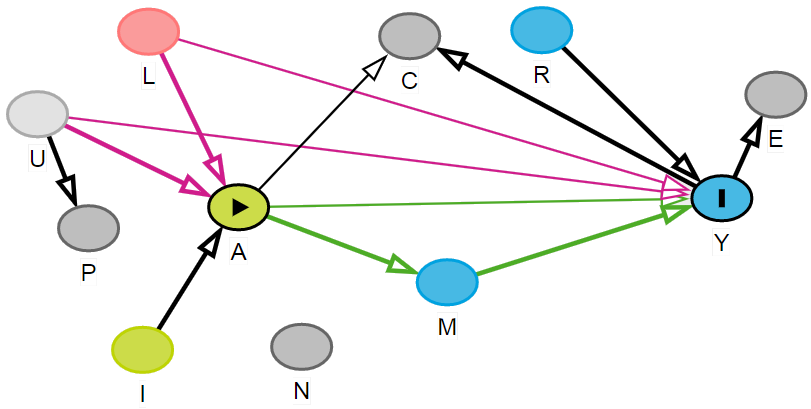
\includegraphics[width=650px]{images/role} \caption{Variable roles: A = exposure or treatment; Y = outcome; L = confounder; R = risk factor for Y; M = mediator; C = collider; E = effect of Y; I = instrument; u = unmeasured confounder; P = proxy of U; N = noise variable}\label{fig:role}
\end{figure}

\begin{itemize}
\tightlist
\item
  Think about the role of variables first

  \begin{itemize}
  \tightlist
  \item
    ideally include confounders to reduce bias
  \item
    consider including risk factor for outcome for greater accuracy
  \item
    IV, collider, mediators, effect of outcome, noise variables should be avoided
  \item
    if something is unmeasured, consider adding proxy (with caution)
  \end{itemize}
\item
  If you do not have subject area expertise, talk to experts
\item
  do pre-screening

  \begin{itemize}
  \tightlist
  \item
    sparse binary variables
  \item
    highly collinear variables
  \end{itemize}
\end{itemize}

\begin{rmdcomment}
Relying on just a blackbox ML method may be dangerous to identify the
roles of variables in the relationship of interest.
\end{rmdcomment}

\hypertarget{why-sl-and-tmle}{%
\section{Why SL and TMLE}\label{why-sl-and-tmle}}

\hypertarget{prediction-goal}{%
\subsection{Prediction goal}\label{prediction-goal}}

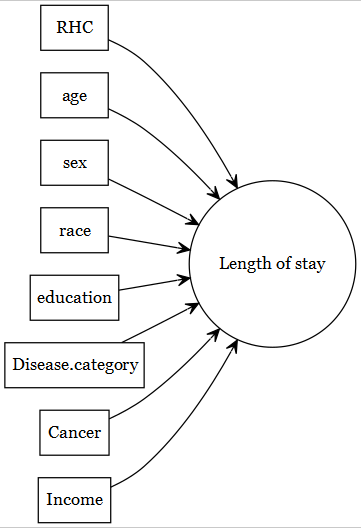
\includegraphics[width=5.01in]{images/dagpred}

\begin{itemize}
\tightlist
\item
  Assuming all covariates are measured, \textbf{parametric models} such as linear and logistic regressions are very efficient, but relies on strong assumptions. In real-world scenarios, it is often hard (if not impossible) to guess the correct specification of the right hand side of the regression equation.
\item
  Machine learning (ML) methods are very helpful for prediction goals. They are also helpful in \textbf{identifying complex functions} (non-linearities and non-additive terms) of the covariates (again, assuming they are measured).
\item
  There are many ML methods, but the procedures are very different, and they come with their own advantages and disadvantages. In a given real data, it is \textbf{hard to apriori predict which is the best ML algorithm} for a given problem.
\end{itemize}

\begin{rmdcomment}
Super learner is helpful in \textbf{combining strength from various
algorithms}, and producing 1 prediction column that has \textbf{optimal
statistical properties}.
\end{rmdcomment}

\hypertarget{causal-inference}{%
\subsection{Causal inference}\label{causal-inference}}

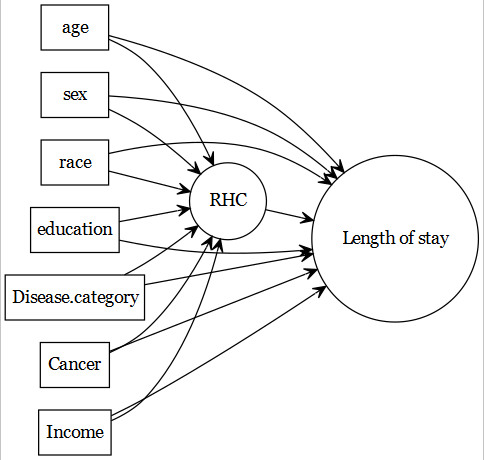
\includegraphics[width=6.72in]{images/dagci}

\begin{itemize}
\tightlist
\item
  For causal inference goals (when we have a primary exposure of interest), machine learning methods are often misleading. This is primarily due to the fact that they usually do not have an inherent mechanism of focusing on \textbf{primary exposure} (RHC in this example); and treats the primary exposure as any other predictors.
\item
  When using g-computation with ML methods, estimation of variance becomes a difficult problem (with correct coverage). Generalized procedures such as \textbf{robust SE or bootstrap methods} are not supported by theory.
\end{itemize}

\begin{rmdcomment}
TMLE method shine, with the help of it's important \textbf{statistical
properties (double robustness, finite sample properties)}.
\end{rmdcomment}

\hypertarget{identifiability-assumptions}{%
\subsection{Identifiability assumptions}\label{identifiability-assumptions}}

However, causal inference requires satisfying identifiability assumptions for us to interpret causality based on association measures from statistical models (see below). Many of these assumptions are not empirically testable. That is why, it is extremely important to work with \textbf{subject area experts} to assess the plausibility of those assumptions in the given context.

\begin{rmdcomment}
No ML method, no matter how fancy it is, can automatically produce
estimates that can be directly interpreted as causal, unless the
identifiability assumptions are properly taken into account.
\end{rmdcomment}

\begin{longtable}[]{@{}lll@{}}
\toprule
\endhead
\begin{minipage}[t]{(\columnwidth - 2\tabcolsep) * \real{0.33}}\raggedright
Conditional Exchangeability\strut
\end{minipage} & \begin{minipage}[t]{(\columnwidth - 2\tabcolsep) * \real{0.33}}\raggedright
\(Y(1), Y(0) \perp A | L\)\strut
\end{minipage} & \begin{minipage}[t]{(\columnwidth - 2\tabcolsep) * \real{0.33}}\raggedright
Treatment assignment is independent of the potential outcome, given covariates\strut
\end{minipage}\tabularnewline
\begin{minipage}[t]{(\columnwidth - 2\tabcolsep) * \real{0.33}}\raggedright
Positivity\strut
\end{minipage} & \begin{minipage}[t]{(\columnwidth - 2\tabcolsep) * \real{0.33}}\raggedright
\(0 < P(A=1 | L) < 1\)\strut
\end{minipage} & \begin{minipage}[t]{(\columnwidth - 2\tabcolsep) * \real{0.33}}\raggedright
Subjects are eligible to receive both treatment, given covariates\strut
\end{minipage}\tabularnewline
\begin{minipage}[t]{(\columnwidth - 2\tabcolsep) * \real{0.33}}\raggedright
Consistency\strut
\end{minipage} & \begin{minipage}[t]{(\columnwidth - 2\tabcolsep) * \real{0.33}}\raggedright
\(Y = Y(a) \forall A=a\)\strut
\end{minipage} & \begin{minipage}[t]{(\columnwidth - 2\tabcolsep) * \real{0.33}}\raggedright
No multiple version of the treatment; and well defined treatment\strut
\end{minipage}\tabularnewline
\bottomrule
\end{longtable}

\hypertarget{further-reading}{%
\section{Further reading}\label{further-reading}}

\hypertarget{key-articles}{%
\subsection{Key articles}\label{key-articles}}

\begin{itemize}
\tightlist
\item
  TMLE Procedure:

  \begin{itemize}
  \tightlist
  \item
    \citet{luque2018targeted}
  \item
    \citet{schuler2017targeted}
  \end{itemize}
\item
  Super learner:

  \begin{itemize}
  \tightlist
  \item
    \citet{rose2013mortality}
  \item
    \citet{naimi2018stacked}
  \end{itemize}
\end{itemize}

\hypertarget{additional-readings}{%
\subsection{Additional readings}\label{additional-readings}}

\begin{itemize}
\tightlist
\item
  \citet{rose2020intersections}
\item
  \citet{snowden2011implementation}
\item
  \citet{naimi2017introduction}
\item
  \citet{austin2015moving}
\item
  \citet{naimi2017challenges}
\item
  \citet{balzer2021demystifying}
\end{itemize}

\hypertarget{workshops}{%
\subsection{Workshops}\label{workshops}}

Highly recommend joining SER if interested in Epi methods development. The following workshops and summer course are very useful.

\begin{itemize}
\tightlist
\item
  \href{https://epiresearch.org/}{SER Workshop} Introduction to Parametric and Semi-parametric Estimators for Causal Inference by Laura B. Balzer \& Jennifer Ahern, 2020
\item
  \href{https://epiresearch.org/}{SER Workshop} Machine Learning and Artificial Intelligence for Causal Inference and Prediction: A Primer by Naimi A, 2021
\item
  \href{https://si.biostat.washington.edu/suminst/archives/SISCER2021/CR2106}{SISCER} Modern Statistical Learning for Observational Data by Marco Carone, David Benkeser, 2021
\end{itemize}

\hypertarget{recorded-webinars}{%
\subsection{Recorded webinars}\label{recorded-webinars}}

The following webinars and workshops are freely accessible, and great for understanding the intuitions, theories and mechanisms behind these methods!

\hypertarget{introductory-materials}{%
\subsubsection{Introductory materials}\label{introductory-materials}}

\begin{itemize}
\tightlist
\item
  \href{https://www.youtube.com/watch?v=8Q9dfW3oOi4}{An Introduction to Targeted Maximum Likelihood Estimation of Causal Effects} by Susan Gruber (Putnam Data Sciences)
\item
  \href{https://www.youtube.com/watch?v=WYnjja8DKPg}{Practical Considerations for Specifying a Super Learner} by Rachael Phillips (Putnam Data Sciences)
\end{itemize}

\hypertarget{more-theory-talks}{%
\subsubsection{More theory talks}\label{more-theory-talks}}

\begin{itemize}
\tightlist
\item
  \href{https://www.youtube.com/watch?v=PrPNP5RVcLg}{Targeted Machine Learning for Causal Inference based on Real World Data} by Mark van der Laan (Putnam Data Sciences)
\item
  \href{https://www.youtube.com/watch?v=1zT17HtvtF8}{An introduction to Super Learning} by Eric Polly (Putnam Data Sciences)
\item
  \href{https://www.youtube.com/watch?v=MDmddX267Ys}{Cross-validated Targeted Maximum Likelihood Estimation (CV-TMLE)} by Alan Hubbard (Putnam Data Sciences)
\item
  \href{https://www.youtube.com/watch?v=2jumfnRQpxs}{Higher order Targeted Maximum Likelihood Estimation} by Mark van der Laan (Online Causal Inference Seminar)
\item
  \href{http://bcooltv.mcgill.ca/FDownloader.aspx?rid=e3143be2-918d-49d9-82ce-4dfea75ef1dc\&DLType=VGAMP4}{Targeted learning for the estimation of drug safety and effectiveness: Getting better answers by asking better questions} by Mireille Schnitzer (CNODES)
\end{itemize}

\hypertarget{more-applied-talks}{%
\subsubsection{More applied talks}\label{more-applied-talks}}

\begin{itemize}
\tightlist
\item
  \href{https://www.youtube.com/watch?v=foY7HoCeo88}{Applications of Targeted Maximum Likelihood Estimation} by Laura Balzar (UCSF Epi \& Biostats)
\item
  \href{https://www.cnodes.ca/online-lecture/targeted-learning-estimation/}{Applying targeted maximum likelihood estimation to pharmacoepidemiology} by Menglan Pang (CNODES)
\end{itemize}

\hypertarget{blog}{%
\subsubsection{Blog}\label{blog}}

\begin{itemize}
\tightlist
\item
  \href{https://www.khstats.com/}{Kat's Stats} by Katherine Hoffman
\item
  \href{https://towardsdatascience.com/targeted-maximum-likelihood-tmle-for-causal-inference-1be88542a749}{towardsdatascience} by Yao Yang
\item
  \href{https://vanderlaan-lab.org/post/}{The Research Group of Mark van der Laan} by Mark van der Laan
\end{itemize}

\hypertarget{refs}{}
\begin{CSLReferences}{0}{0}
\end{CSLReferences}

  \bibliography{book.bib,packages.bib}

\end{document}
